%%
%% TeX:UTF-8
%%
%% POSTECH Master's Thesis - Hyunho Kook
%%
%% MP-Init & TrSG: Stabilizing Direct Training of SNNs
%%

% @class    postech-ucs.cls
% @options  master, english, final
% - master  : 석사과정 (3-member committee)
% - english : 영문논문 (본문은 영어, 국문요약 별도)
% - final   : 최종판 (앞표지/속표지/제출승인서/심사완료검인 자동생성)
% - pdfdoc  : (선택) 북마크/colorlink 활성화
\documentclass[master,english,final]{postech-ucs}

%% ─────────────────────────────────────────────────────────────────────
%%  Packages required for the imported WACV manuscript
%% ─────────────────────────────────────────────────────────────────────
\usepackage{amsmath,amssymb,amsthm}
\usepackage{enumitem}
\usepackage{algorithm}
\usepackage{algpseudocode}
\usepackage{comment}
\usepackage{anyfontsize}
\usepackage{caption}
\usepackage{subcaption}
\usepackage{multirow}
\usepackage{makecell}
\usepackage{boldline}
\usepackage{pifont}
\usepackage{dsfont}
\usepackage{wrapfig}
\usepackage{booktabs}
\usepackage{tikz}
\usepackage{pgfplots}
\pgfplotsset{compat=1.18}
\usepackage{xcolor}
\usepackage{cleveref}

%% Cross-reference labels: capitalize for sentence start
\crefname{section}{Section}{Sections}
\crefname{subsection}{Section}{Sections}
\crefname{chapter}{Chapter}{Chapters}
\crefname{figure}{Figure}{Figures}
\crefname{table}{Table}{Tables}
\crefname{equation}{Eq.}{Eqs.}
\crefname{algorithm}{Algorithm}{Algorithms}

%% Theorem/Lemma/Assumption environments (used in MP-Init chapter)
\newtheorem{theorem}{Theorem}[chapter]
\newtheorem{lemma}[theorem]{Lemma}
\newtheorem{assumption}{Assumption}[chapter]
\newtheorem{proposition}[theorem]{Proposition}

%% Inline annotation helpers carried over from WACV preamble
\newcommand{\red}[1]{{\color{red}#1}}
\newcommand{\todo}[1]{{\color{red}#1}}
\newcommand{\TODO}[1]{\textbf{\color{red}[TODO: #1]}}
\definecolor{mypink}{rgb}{0.858, 0.188, 0.478}

%% Math operators used in the thesis
\newcommand{\argmax}{\operatornamewithlimits{arg\,max}}

%% Allow LaTeX to find figures inside the WACV source tree without copying.
\graphicspath{{./}{_WACV2026__MPInit_TrSG/}}

%% ─────────────────────────────────────────────────────────────────────
%%  Document metadata
%% ─────────────────────────────────────────────────────────────────────

% @command title 논문 제목 / Thesis title
\title[korean]{스파이킹 신경망의 직접 학습 안정화를 위한 막전위 초기화와 임계값 강건성 기반 서러게이트 그래디언트}
\title[english]{Enhancing Stability in Direct Training of Spiking Neural Networks through Membrane Potential Initialization and Threshold-Robust Surrogate Gradients}

% @command author 저자
% Korean ㄱ분과 영문 표기
\author[korean]{국}{현 호}
\author[english]{Kook}{Hyunho}

% @command advisor (석사: 단독 지도교수)
\advisor[major]{박 은 혁}{Eunhyeok Park}{signed}

% @command department {학과 코드}{학위종류}
% CSE = 컴퓨터공학과, science = Master of Science
\department{CSE}{science}

% @command studentid 학번
\studentid{20242015}

% @command referee 심사위원 (석사 = 위원장 포함 3인)
\referee[1]{Eunhyeok Park}      % 심사위원장 (지도교수)
\referee[2]{Jungseul Ok}        % 심사위원
\referee[3]{Jae-Joon Kim}       % 심사위원

% @command approvaldate / refereedate / gradyear
% TODO: 실제 일자 확정 후 수정
\approvaldate{2026}{05}{18}
\refereedate{2026}{05}{18}
\gradyear{2026}

%% ─────────────────────────────────────────────────────────────────────
%%  Body
%% ─────────────────────────────────────────────────────────────────────
\begin{document}

    %% 앞표지·속표지·제출승인서·심사완료검인서는 final 옵션으로 자동 생성됨

    % 영문 초록 (1,000 단어 이내)
    \begin{abstract}
        %% English Abstract — appears immediately after the cover pages.
%% Within \begin{abstract} ... \end{abstract} environment provided by postech-ucs.cls.
%% Limit: 1,000 words (지침 1.나.③)

Recent advancements in the direct training of Spiking Neural Networks (SNNs) have demonstrated high-quality outputs even at early timesteps, paving the way for novel energy-efficient AI paradigms. However, the inherent non-linearity and temporal dependencies in SNNs introduce persistent challenges, such as temporal covariate shift (TCS) and unstable gradient flow with learnable neuron thresholds.

In this thesis, we enhance the stability of direct SNN training through two key innovations: \textbf{MP-Init (Membrane Potential Initialization)} and \textbf{TrSG (Threshold-Robust Surrogate Gradient)}. MP-Init addresses TCS by aligning the initial membrane potential with its stationary distribution, while TrSG stabilizes gradient flow with respect to the threshold voltage during training. We provide a rigorous mathematical analysis of both methods, prove the geometric convergence of the membrane potential to a stationary distribution, and characterize the threshold-induced gradient pathologies of existing surrogate-gradient families.

Extensive experiments validate our approach, achieving state-of-the-art accuracy on both static (CIFAR-10/100, ImageNet) and dynamic (DVS-CIFAR10) image datasets, while incurring negligible parameter and computational overhead. The methods further generalize cleanly to Transformer-based SNNs and to event-based object detection, indicating broad applicability beyond the classification setting.

The code for reproducing the results is available at: \href{https://github.com/kookhh0827/SNN-MP-Init-TRSG}{\textcolor{mypink}{https://github.com/kookhh0827/SNN-MP-Init-TRSG}}.

    \end{abstract}

    % 백색별지는 abstract 뒤에 자동 삽입됨 (postech-ucs.cls v0.7+)

    % 목차
    \tableofcontents

    % 그림목차
    \listoffigures

    % 표목차
    \listoftables

    %% ─────────────────────────────────────────────────────────────
    %%  Main body
    %% ─────────────────────────────────────────────────────────────
    \chapter{Introduction}
\label{ch:introduction}

\section{Motivation}
\label{sec:intro_motivation}

Modern deep neural networks (DNNs) have achieved remarkable accuracy across vision, language, and multimodal tasks, but their energy footprint has grown substantially as model scale has increased. Training and serving large foundation models routinely consumes megawatt-scale power, and even moderately sized inference workloads on edge devices remain difficult to deploy under tight energy budgets. This trajectory motivates a search for fundamentally more efficient computation models.

Spiking Neural Networks (SNNs) offer one such alternative. By transmitting information through discrete spikes over time, SNNs enable efficient, event-driven processing~\cite{cao:2015, esser:2016, neftci:2018, roy:2019, cramer:2022, rathi:2023}, especially when paired with neuromorphic hardware~\cite{merolla:2014, akopyan:2015, davies:2018}. Recent advances in direct training~\cite{wu:2018, wu:2019} have significantly improved SNN accuracy with only a handful of timesteps, narrowing the historical efficiency-vs.-accuracy gap. Yet, SNNs still lag behind conventional deep neural networks, and their complex temporal dynamics often hinder performance on large-scale datasets~\cite{review_guo:2023, review_zhou:2024}. Further innovations are therefore crucial to ensure reliability and accuracy for real-world adoption.

\section{Challenges in Direct Training of SNNs}
\label{sec:intro_challenges}

This thesis identifies and addresses two challenges that, despite extensive prior work, remain insufficiently understood.

\paragraph{Challenge 1: Temporal Covariate Shift (TCS).}
The first challenge is \textbf{Temporal Covariate Shift (TCS)}~\cite{bntt:2020}, in which internal covariate shifts in activations accumulate over time. Existing remedies such as TEBN~\cite{tebn:2022} and TAB~\cite{tab:2024} introduce timestep-specific normalization parameters, but they disrupt parameter homogeneity across time and increase both model complexity and computational cost. More importantly, our analysis reveals that these methods fail to mitigate TCS in the membrane potential of leaky-integrate-and-fire (LIF) neurons. Since the membrane potential directly determines neuronal output, neglecting TCS in this component leads to significant accuracy degradation.

\paragraph{Challenge 2: Gradient pathology of learnable thresholds.}
The second challenge concerns \textbf{training the internal parameters}~\cite{fang:2021, wang:2022, rathi:2023} of LIF neurons—chiefly the threshold voltage $V_{\text{thr}}$ and the leakage term $\tau$. Despite their crucial role in LIF neuron behavior, these parameters are typically fixed or updated under strict constraints. We show that existing surrogate-gradient flow heavily depends on the scale of $V_{\text{thr}}$, and that unconstrained updates during training lead to either gradient flooding/starvation or gradient explosion/vanishing. To our knowledge, this issue has not been explicitly recognized prior to this work.

\section{Contributions}
\label{sec:intro_contributions}

This thesis makes the following contributions:

\begin{itemize}[leftmargin=2em]
    \item \textbf{MP-Init (Membrane Potential Initialization).} We trace TCS to the mismatch between the initial membrane potential and its stationary distribution. We prove a discrete-time convergence theorem (Markov-chain Doeblin minorization) showing that the layer-wise membrane potential converges geometrically to a unique stationary distribution under mild assumptions. Building on this, we propose a per-layer running-mean initialization that aligns the initial membrane potential with the stationary mean, eliminating TCS while preserving the standard inference pipeline of LIF SNNs.

    \item \textbf{TrSG (Threshold-robust Surrogate Gradient).} We classify existing surrogate gradients into Absolute-Scale (AS-SG) and Relative-Scale (RS-SG) families, and analyze how each becomes unstable when $V_{\text{thr}}$ is trainable. We then propose TrSG, which keeps the relative-scale active window while canceling the destabilizing $1/V_{\text{thr}}$ factor through a threshold-multiplied forward path. The result is a gradient whose magnitude is invariant to the threshold scale and whose active region adapts naturally with $V_{\text{thr}}$.

    \item \textbf{Comprehensive empirical validation.} On CIFAR-10/100, ImageNet, and DVS-CIFAR10, our combined method achieves state-of-the-art accuracy at competitive timesteps. We further demonstrate that MP-Init and TrSG transfer cleanly to Transformer-based SNN backbones and to event-based object detection, indicating broad applicability.\footnote{The reference implementation that reproduces the results in this thesis is available at \href{https://github.com/kookhh0827/SNN-MP-Init-TRSG}{\texttt{https://github.com/kookhh0827/SNN-MP-Init-TRSG}}.}
\end{itemize}

\section{Thesis Organization}
\label{sec:intro_organization}

The remainder of this thesis is organized as follows.
\Cref{ch:background} reviews the background and related work in spiking neural networks, including direct-training methodologies, prior approaches to TCS, and existing strategies for learning internal LIF parameters.
\Cref{ch:preliminaries} fixes notation and formalizes the LIF neuron model, the surrogate gradient framework, and the active-neuron convention used throughout the thesis.
\Cref{ch:mpinit} introduces \textbf{MP-Init}: it identifies the root cause of TCS in the membrane potential, presents a rigorous convergence theorem, and develops the running-mean initialization algorithm.
\Cref{ch:trsg} introduces \textbf{TrSG}: it analyzes the threshold sensitivity of existing surrogate gradients, derives the threshold-robust formulation, and provides a detailed gradient analysis with respect to $V_{\text{thr}}$ and $\tau$.
\Cref{ch:experiments} reports experimental results on static and event-based datasets, ablation studies, comparisons with state-of-the-art methods, and extensions to advanced architectures and downstream tasks.
\Cref{ch:conclusion} concludes with a discussion of limitations and directions for future work.

    \chapter{Background and Related Work}
\label{ch:background}

This chapter situates the contributions of the thesis within the broader literature. We first review the biological motivation and hardware platforms that have made spiking neural networks (SNNs) attractive (\cref{sec:bg_snn}). We then survey direct-training methodologies (\cref{sec:bg_direct}), existing approaches to temporal covariate shift (\cref{sec:bg_tcs}), and prior work on learning the internal parameters of LIF neurons (\cref{sec:bg_internal}).

\section{Spiking Neural Networks}
\label{sec:bg_snn}

\subsection{Biological Motivation}
\label{subsec:bg_bio}
Biological neurons communicate through asynchronous, all-or-none electrical events called \emph{spikes}. The leaky integrate-and-fire (LIF) abstraction captures the essential dynamics: a neuron integrates incoming current onto its membrane potential, leaks toward a resting value, and emits a spike whenever the membrane potential crosses a threshold. Notably, recent neuroscience evidence~\cite{yoo:2023} indicates that resting membrane potentials differ across distinct cortical regions: neurons in the prefrontal cortex (PFC) exhibit approximately 10~mV higher resting potentials than those in the posterior parietal cortex (PPC), driven by region-specific recurrent synaptic strengths mediated by NMDA receptors. This regional variability in resting potentials motivates the per-layer initialization strategy adopted in this thesis (\cref{ch:mpinit}).

\subsection{Neuromorphic Hardware}
\label{subsec:bg_hw}
Several specialized accelerators exploit the event-driven nature of spiking computation: TrueNorth~\cite{merolla:2014, akopyan:2015}, Loihi~\cite{davies:2018}, and emerging digital/mixed-signal designs all process spikes asynchronously and skip computation for inactive neurons, yielding orders-of-magnitude lower energy than dense matrix-multiplication accelerators. A practical consequence is that SNN training methods that introduce extra timestep-dependent state, or that depart from the canonical LIF inference pipeline, can be difficult to deploy. The methods in this thesis preserve the standard LIF inference pipeline so that hardware compatibility is unaffected (cf.~\cref{subsec:trsg_inference}).

\section{Direct Training of SNNs}
\label{sec:bg_direct}

Surrogate gradient (SG) descent enables end-to-end training of SNNs by approximating the non-differentiable firing function~\cite{lee:2016, wu:2018, wu:2019}. Some studies focus on the impact of hyperparameters and the shape of surrogate derivatives~\cite{zenke:2021, li:2021}, while more recent advances introduce differentiable surrogate gradient functions~\cite{li:2021} and Temporal Efficient Training (TET) losses~\cite{deng:2022}. Other approaches regulate the membrane potential through additional loss terms~\cite{guo:2022, guo:2023} or through batch-normalization variants~\cite{guo:2023_2}. Methods that modify LIF dynamics themselves~\cite{fang:2023, yao:2022, huang:2024} have also been explored, although they may be incompatible with existing neuromorphic hardware~\cite{hunsberger:2015, review_guo:2023}.

\section{Temporal Covariate Shift}
\label{sec:bg_tcs}

The TCS problem was first identified in BNTT~\cite{bntt:2020} and later addressed by methods such as TEBN~\cite{tebn:2022} and TAB~\cite{tab:2024}, which adapt normalization layers on a per-timestep basis. While these methods alleviate TCS in activations, they increase model complexity with additional parameters and, more critically, overlook the persistent shift in membrane potential, a primary source of TCS during inference (see \cref{sec:mpinit_root}).

IMP+LTS~\cite{shen:2024} proposed training the initial membrane potential for every neuron to enhance representational power. However, it does not directly address TCS and incurs a large parameter overhead scaling with the number of neurons $\mathcal{O}(N)$. By contrast, our approach initializes membrane potentials at the layer level $\mathcal{O}(L)$ ($L \ll N$), directly targeting TCS while remaining lightweight.

More recently, MPS~\cite{ding:2025} reinterpreted SNNs from an ensemble-learning perspective, arguing that excessive differences in membrane potential distributions across timesteps destabilize subnetworks. Their smoothing and guidance strategies improve temporal consistency and yield accuracy gains; however, these methods modify the LIF update rule itself and require additional smoothing coefficients and guidance losses. Both training and inference therefore diverge from the standard LIF neuron model. In contrast, our approach preserves the original inference pipeline: MP-Init adds negligible overhead during training while inference remains compatible with neuromorphic hardware~\cite{davies:2018}.

\section{Learning Internal Parameters of LIF Neurons}
\label{sec:bg_internal}

Recent studies have explored training internal parameters such as the threshold voltage and the leakage term via gradient descent~\cite{fang:2021, wang:2022, rathi:2023}. PLIF~\cite{fang:2021} optimizes the leakage term, LTMD~\cite{wang:2022} adjusts the threshold voltage, and DIET-SNN~\cite{rathi:2023} learns both. However, these works provide limited analysis of the gradient flow associated with learnable parameters, leaving questions about training stability unanswered. In contrast, we find that when the threshold voltage becomes trainable, surrogate-gradient methods can exhibit instability—producing misaligned, exploding, or vanishing gradients (\cref{sec:trsg_two_families}). To overcome these issues we propose, in \cref{ch:trsg}, a novel surrogate-gradient formulation that remains stable when learning the threshold voltage and ensures robust convergence.

\section{Summary}
\label{sec:bg_summary}

Existing methods either (i) address TCS only at the activation level while ignoring its origin in the membrane potential, or (ii) train the threshold voltage without a principled treatment of the resulting gradient pathology. The remainder of this thesis closes both gaps.

    \chapter{Preliminaries}
\label{ch:preliminaries}

This chapter fixes the notation used throughout the thesis. We introduce the discrete-time leaky integrate-and-fire (LIF) neuron model (\cref{sec:prelim_lif}) and clarify the convention by which silent neurons are excluded from our statistical analyses (\cref{sec:prelim_active}).

\section{The LIF Neuron Model}
\label{sec:prelim_lif}

The LIF model~\cite{eshraghian:2021} is a widely used spiking neural model that captures key behaviors of biological neurons, including spike firing and membrane-potential decay. In discrete time $t \in \mathbb{N}$, the LIF neuron's behavior is described by the following three equations.

\noindent\textbf{Membrane integration.}
\begin{equation}
\label{eq:lif_discrete_potential}
    M^{l}[t] \;=\; \left( 1 - \frac{1}{\tau^{l}} \right) U^{l}[t-1] + \frac{1}{\tau^{l}} I^{l}_{\text{in}}[t],
\end{equation}

\noindent\textbf{Spike generation.}
\begin{equation}
\label{eq:lif_discrete_firing}
    S^{l}[t] \;=\; \mathcal{H}\!\left( M^{l}[t] - V^{l}_{\text{thr}} \right),
\end{equation}

\noindent\textbf{Reset.}
\begin{equation}
\label{eq:lif_discrete_reset}
    U^{l}[t] \;=\; \begin{cases}
        M^{l}[t] - V^{l}_{\text{thr}} \cdot S^{l}[t], & \text{(soft reset)} \\
        M^{l}[t] \cdot (1 - S^{l}[t]). & \text{(hard reset)}
\end{cases}
\end{equation}

\noindent
Here $l$ is the layer index, $\mathcal{H}(\cdot)$ is the Heaviside step function, $M^{l}[t]$ is the post-integration membrane potential, $U^{l}[t]$ is the post-reset membrane potential, $S^{l}[t]\in\{0,1\}$ is the spike output, $V^{l}_{\text{thr}}$ is the threshold voltage, and $\tau^{l}$ is the leakage time constant. The presynaptic input current is
\[
I^{l}_{\text{in}}[t] \;=\; W_{l-1}^{l}\,O^{l-1}[t],
\]
where $W_{l-1}^{l}$ is the synaptic weight matrix from layer $l-1$ to $l$, and $O^{l-1}[t]$ is the output of the previous layer. In direct training, this output typically equals the binary spike itself, $O^{l}[t] = S^{l}[t]$~\cite{wu:2018}. Following standard practice~\cite{eshraghian:2021}, the leakage constant $\tau^{l}$ can be absorbed into the synaptic weights via the rescaling $W_{l-1}^{l} \!:=\! \tfrac{1}{\tau^{l}} W_{l-1}^{l}$ in \cref{eq:lif_discrete_potential}.

\paragraph{Soft vs.\ hard reset.}
The choice between soft and hard reset in \cref{eq:lif_discrete_reset} affects post-firing dynamics. Under a soft reset~\cite{rueckauer:2016}, the membrane potential decreases by $V^{l}_{\text{thr}}$ when a spike fires; under a hard reset~\cite{wu:2018}, the membrane potential resets to zero. Both regimes are widely used in the literature, and the methods proposed in this thesis are effective in either case.

\section{Active Neurons and Silent Neurons}
\label{sec:prelim_active}

In our analysis of TCS we focus only on \emph{active neurons}, i.e., those that fire at least once during each simulation. Prior work~\cite{yin:2022} shows that a substantial fraction of neurons in trained SNNs remain subthreshold throughout a simulation; we refer to these as \emph{silent} neurons. Silent neurons are irrelevant to our statistical analysis: they neither contribute to information propagation nor exhibit statistical properties similar to those of active neurons. Therefore, when computing membrane-potential statistics in this thesis, we exclude silent neurons.

\section{Notation Summary}
\label{sec:prelim_notation}

\Cref{tab:notation} summarizes the symbols used throughout the thesis.

\begin{table}[h!]
\centering
\small
\begin{tabular}{l l}
\toprule
\textbf{Symbol} & \textbf{Meaning} \\
\midrule
$l$ & Layer index \\
$t$ & Discrete timestep \\
$M^{l}[t]$ & Post-integration membrane potential at layer $l$, time $t$ \\
$U^{l}[t]$ & Post-reset membrane potential \\
$S^{l}[t]\in\{0,1\}$ & Spike output \\
$O^{l}[t]$ & Layer output (typically $=S^{l}[t]$ in direct training) \\
$V^{l}_{\text{thr}}$ & Threshold voltage at layer $l$ \\
$\tau^{l}$ & Leakage time constant at layer $l$ \\
$I^{l}_{\text{in}}[t]$ & Presynaptic input current \\
$W_{l-1}^{l}$ & Synaptic weight matrix from layer $l\!-\!1$ to $l$ \\
$\mathcal{H}(\cdot)$ & Heaviside step function \\
$\pi$ & Stationary distribution of $U[t]$ (Markov chain) \\
$T$ & Total number of timesteps in the simulation window \\
\bottomrule
\end{tabular}
\caption{Notation used throughout this thesis.}
\label{tab:notation}
\end{table}

    \chapter{Membrane Potential Initialization (MP-Init)}
\label{ch:mpinit}

This chapter presents \textbf{MP-Init}, the first contribution of this thesis. \Cref{sec:mpinit_motivation} motivates the method by examining why existing TCS remedies are insufficient. \Cref{sec:mpinit_root,sec:mpinit_empirical} empirically and theoretically pinpoint the root cause of TCS in the \emph{membrane potential}, and \cref{sec:mpinit_theorem,sec:mpinit_lemma} establish the convergence properties used to derive the algorithm in \cref{sec:mpinit_algorithm}. \Cref{sec:mpinit_bio} discusses biological plausibility, and \cref{sec:mpinit_summary} closes the chapter.

\section{Motivation}
\label{sec:mpinit_motivation}

TCS~\cite{bntt:2020, tebn:2022, tab:2024} limits the performance of SNNs during inference, particularly when batch normalization (BN) is employed. Despite BN's capability to normalize activations during training, the fixed normalization statistics used at inference cause activation drift across timesteps and accuracy degradation. Previous methods~\cite{tebn:2022, tab:2024} have tried to address this issue through timestep-dependent normalization, but these approaches remain superficial: they fail to resolve the underlying cause—drift in the membrane potential of LIF neurons.

To tackle this issue, we propose \textbf{MP-Init (Membrane Potential Initialization)}, an efficient method that directly targets TCS in the membrane potential. MP-Init ensures stable activation distributions throughout inference by initializing the membrane potential of spiking neurons in each layer to match its stationary distribution. This eliminates the need for timestep-dependent normalization and improves final performance by aligning training and inference statistics.

\section{Empirical Evidence: TCS in the Membrane Potential}
\label{sec:mpinit_empirical}

\begin{figure}[t!]
  \centering
  \begin{subfigure}{0.495\linewidth}
    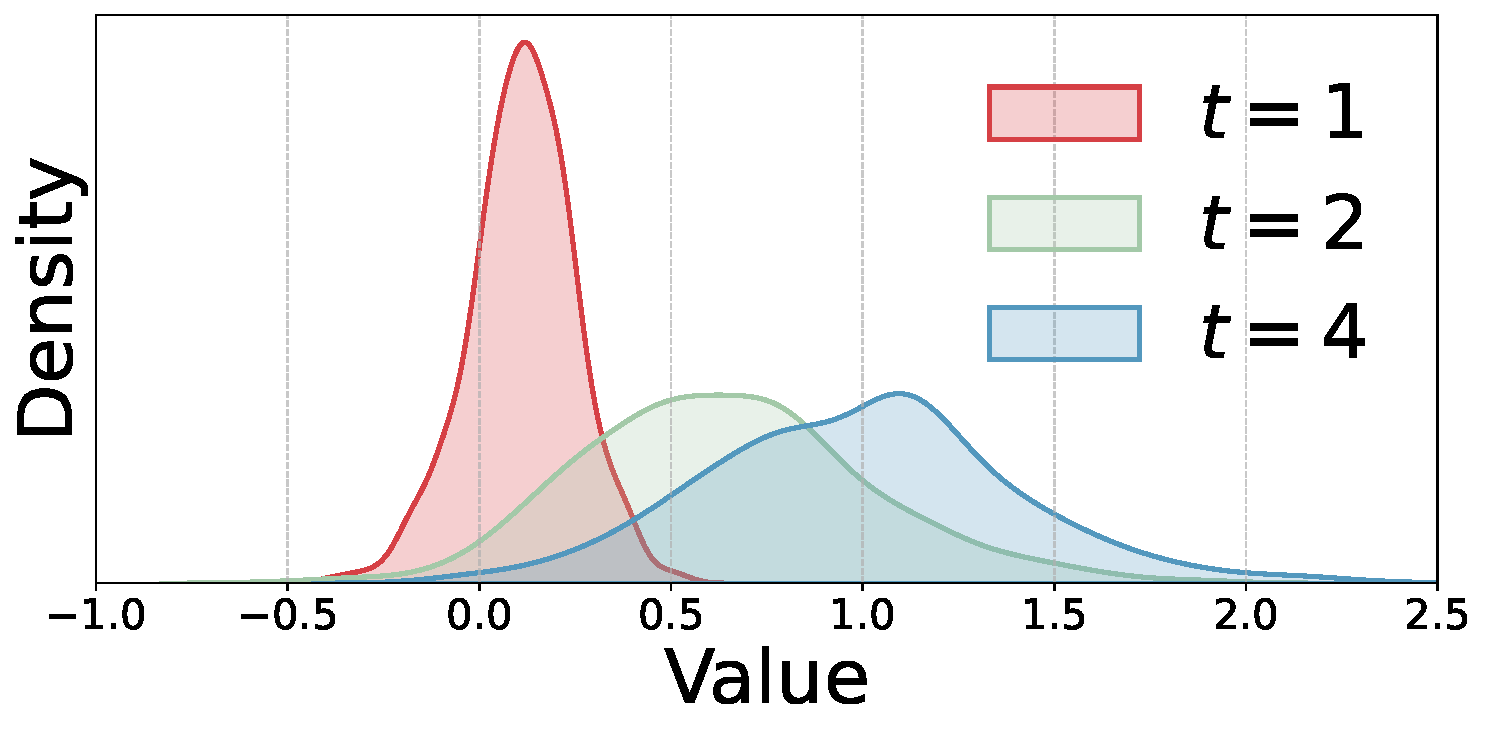
\includegraphics[width=0.95\linewidth]{fig/density_plot_membrane_potential_tdbn.pdf}
    \caption{tdBN}
    \label{fig:membrane_potential_a}
  \end{subfigure}
  \hfill
  \begin{subfigure}{0.495\linewidth}
    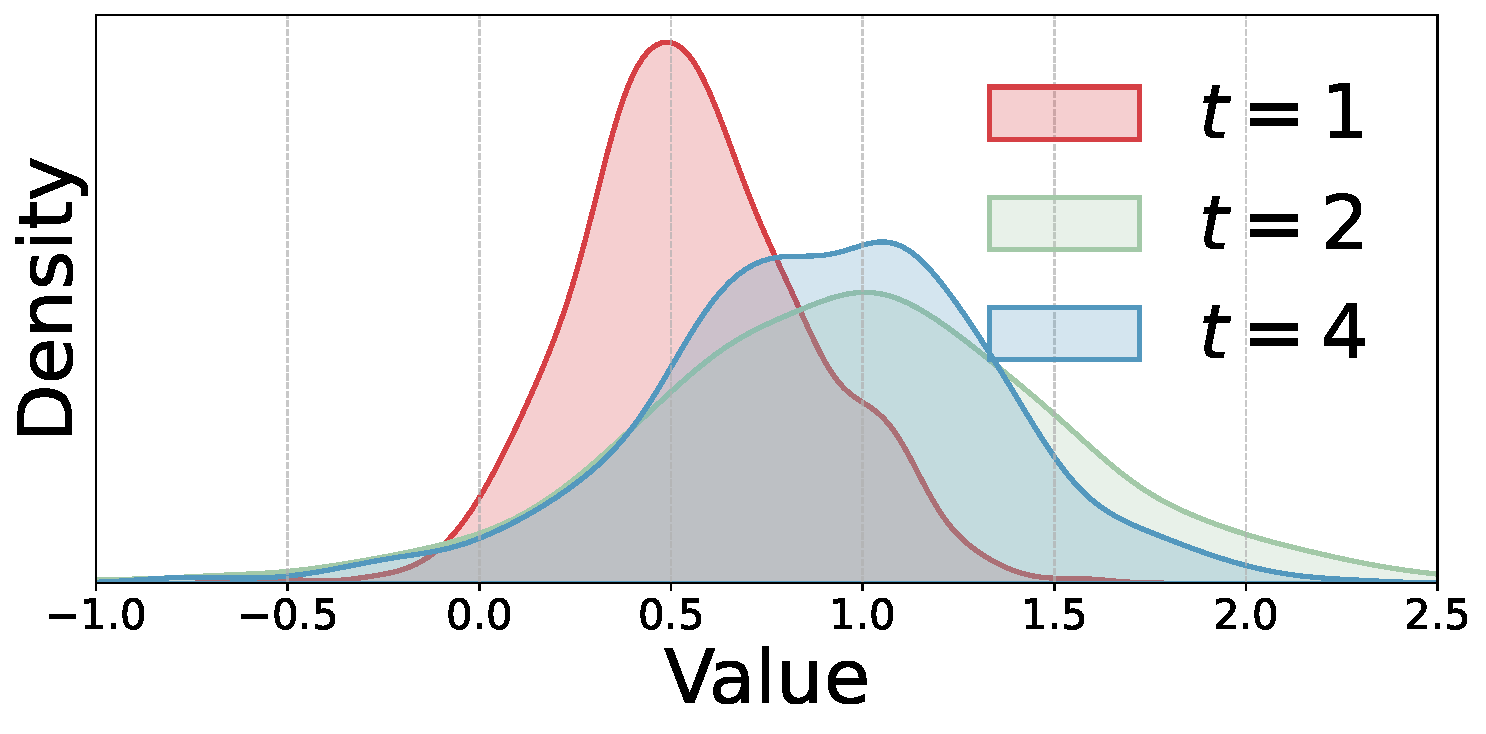
\includegraphics[width=0.95\linewidth]{fig/density_plot_membrane_potential_tebn.pdf}
    \caption{TEBN}
  \end{subfigure}
  \begin{subfigure}{0.495\linewidth}
    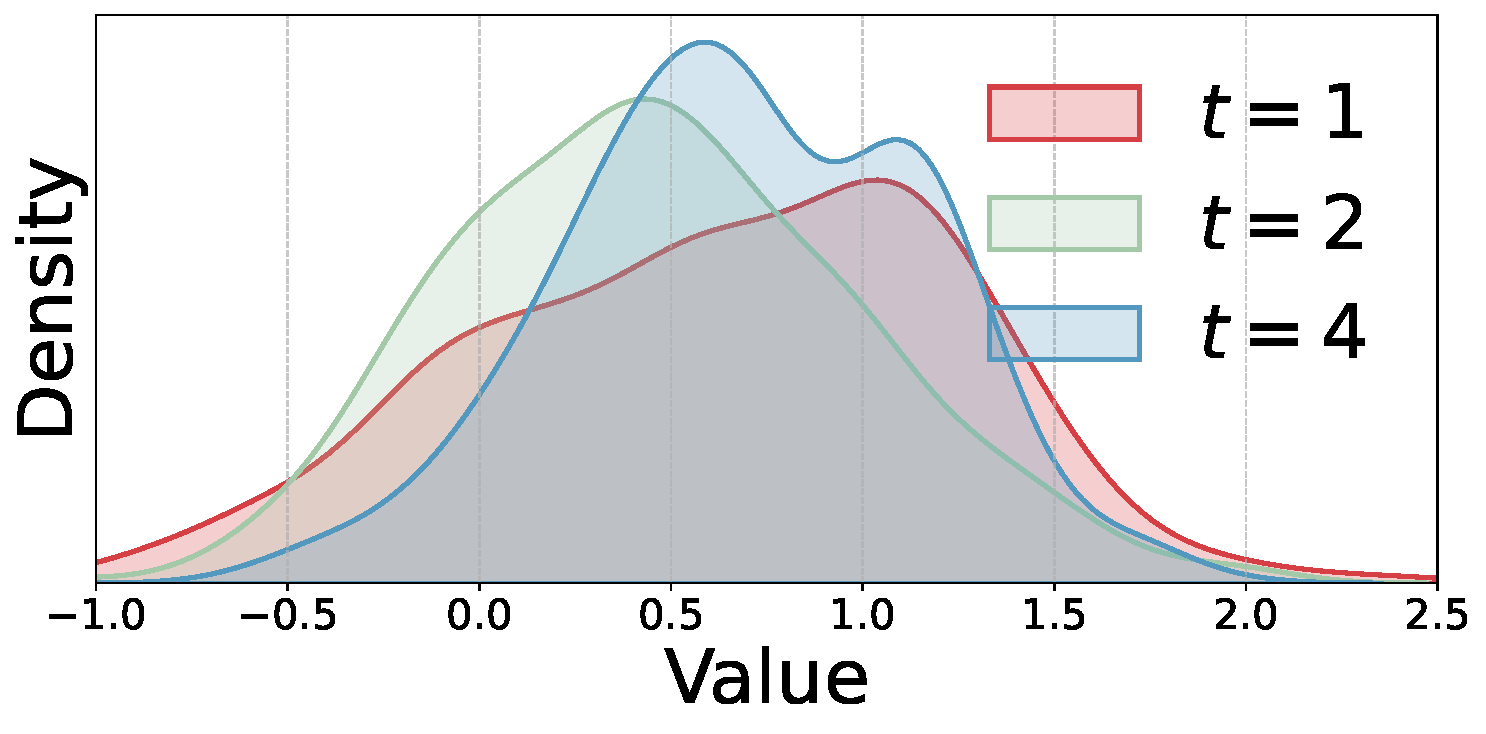
\includegraphics[width=0.95\linewidth]{fig/density_plot_membrane_potential_tab.pdf}
    \caption{TAB}
  \end{subfigure}
  \hfill
  \begin{subfigure}{0.495\linewidth}
    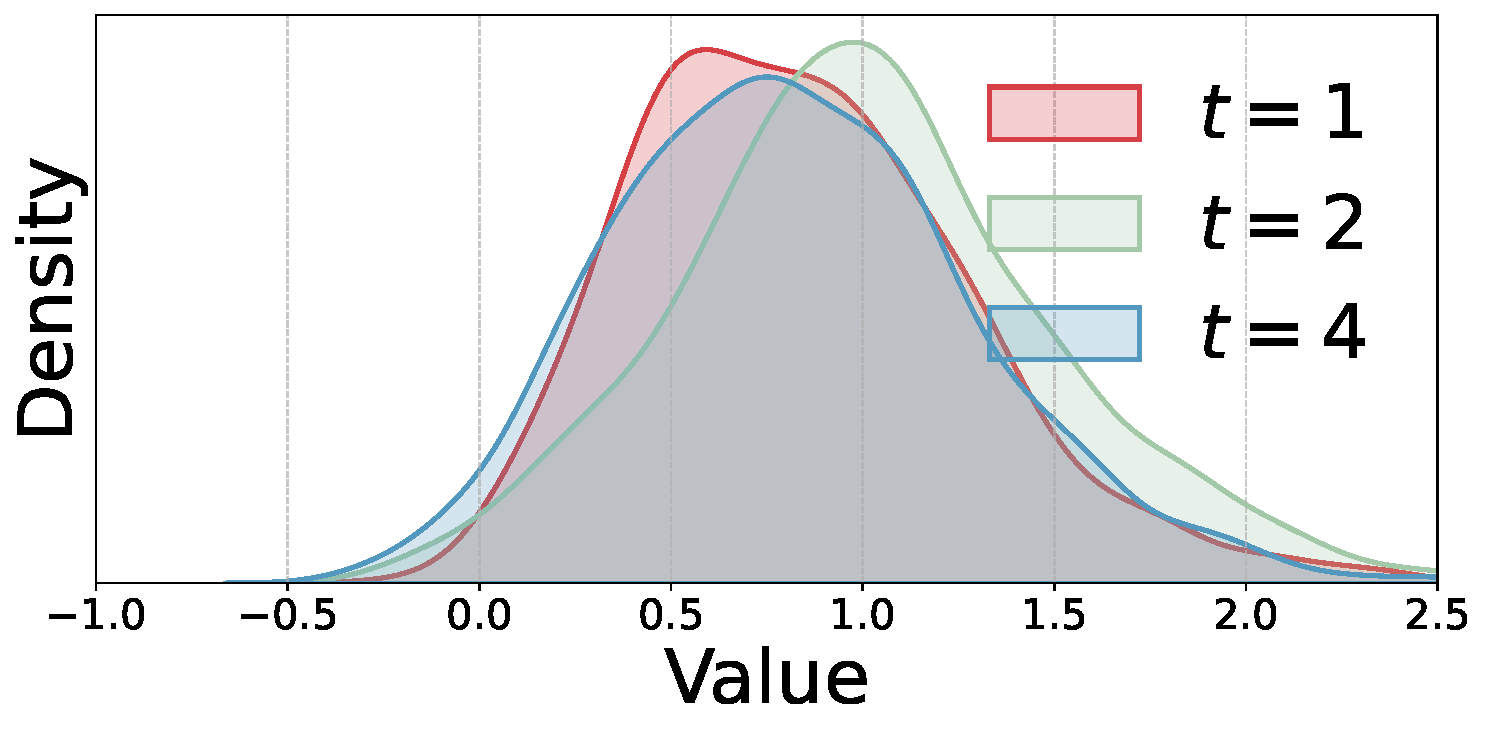
\includegraphics[width=0.95\linewidth]{fig/density_plot_membrane_potential_mpinit.pdf}
    \caption{MP-Init (ours)}
  \end{subfigure}
  \caption{Membrane potential distributions across timesteps at the third spiking layer of ResNet-19 on CIFAR-100. Existing TCS-aware normalizations (TEBN, TAB) still leave a temporal drift in the membrane potential, while MP-Init aligns the per-timestep distributions.}
  \label{fig:combined_membrane}
\end{figure}

\begin{figure}[t!]
  \centering
  \begin{subfigure}{0.495\linewidth}
    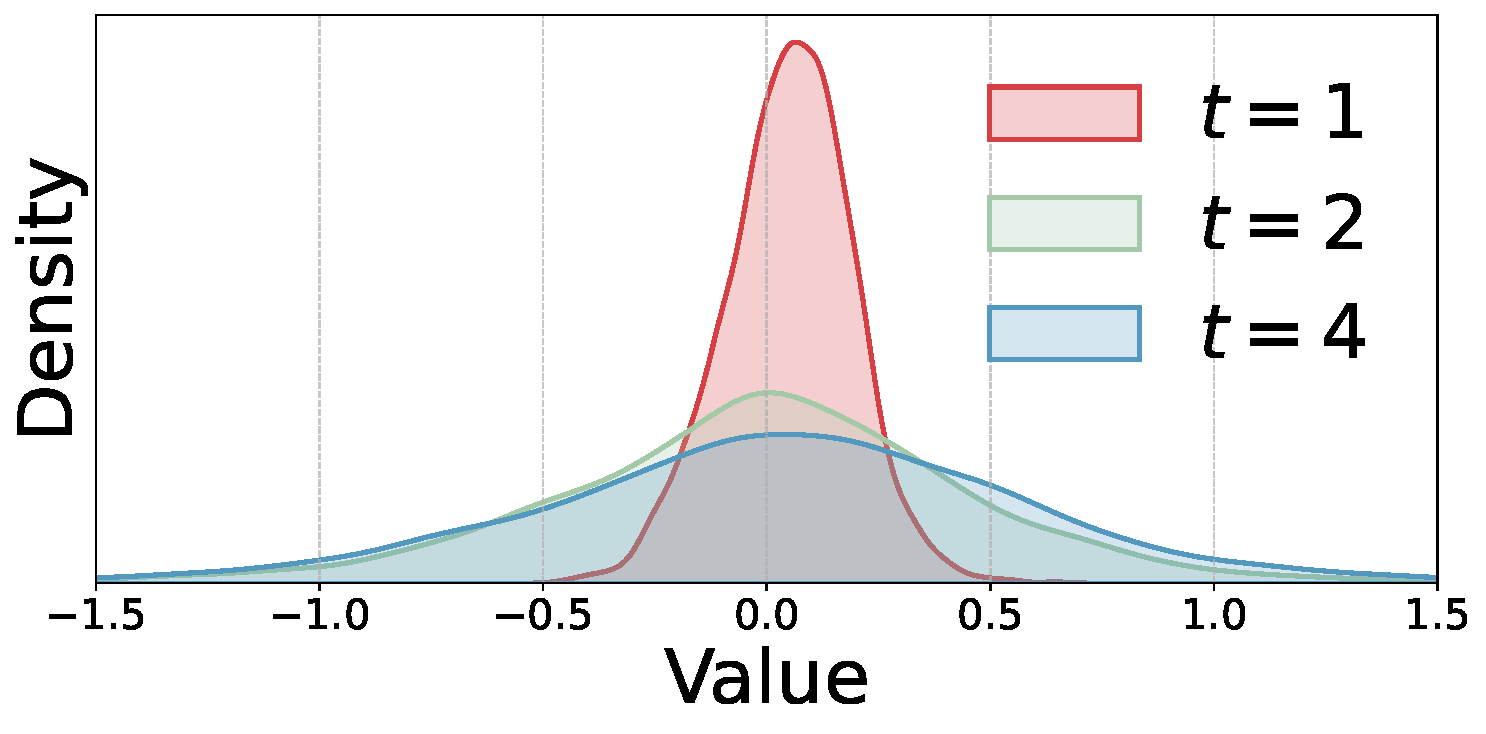
\includegraphics[width=0.95\linewidth]{fig/density_plot_presynaptic_input_tdbn.pdf}
    \caption{tdBN}
    \label{fig:presynaptic_input_a}
  \end{subfigure}
  \hfill
  \begin{subfigure}{0.495\linewidth}
    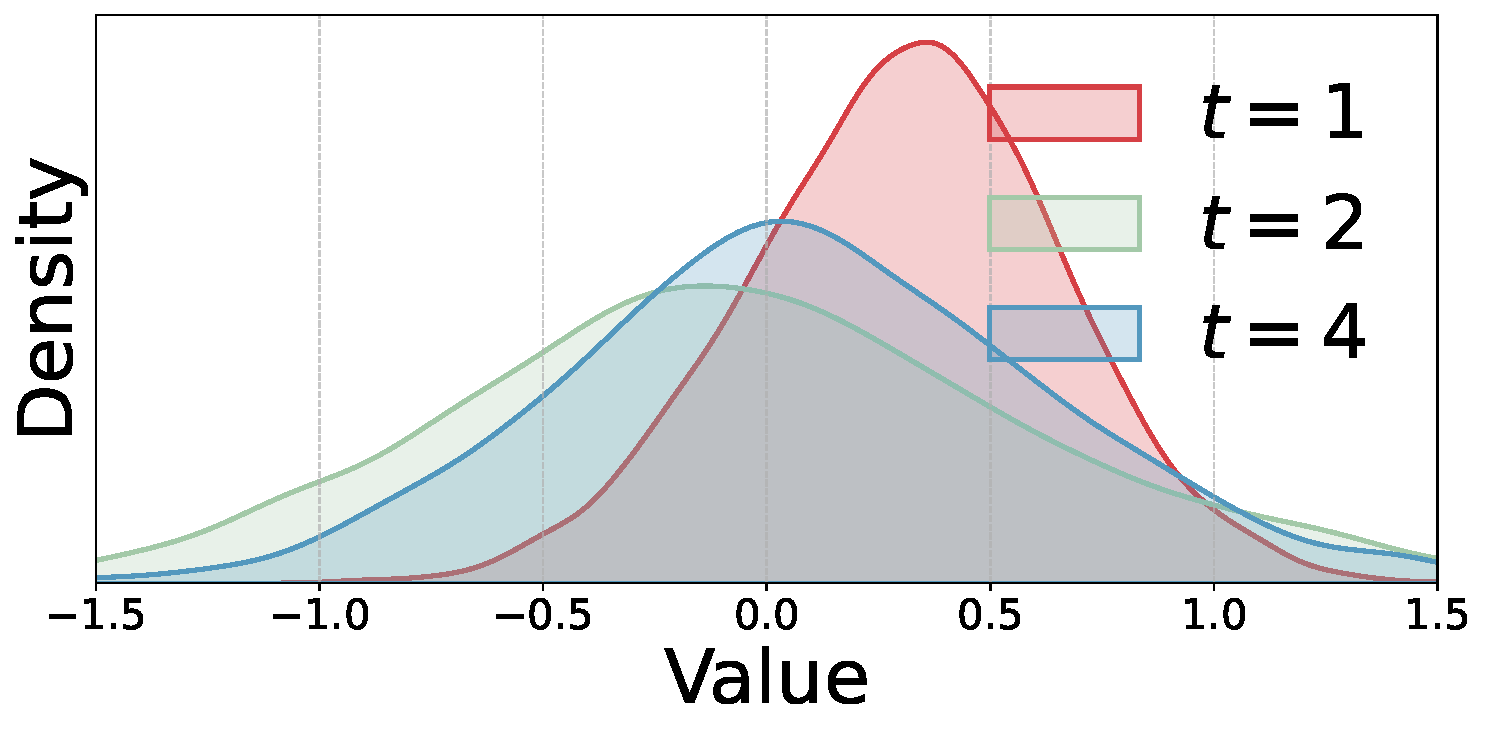
\includegraphics[width=0.95\linewidth]{fig/density_plot_presynaptic_input_tebn.pdf}
    \caption{TEBN}
  \end{subfigure}
  \begin{subfigure}{0.495\linewidth}
    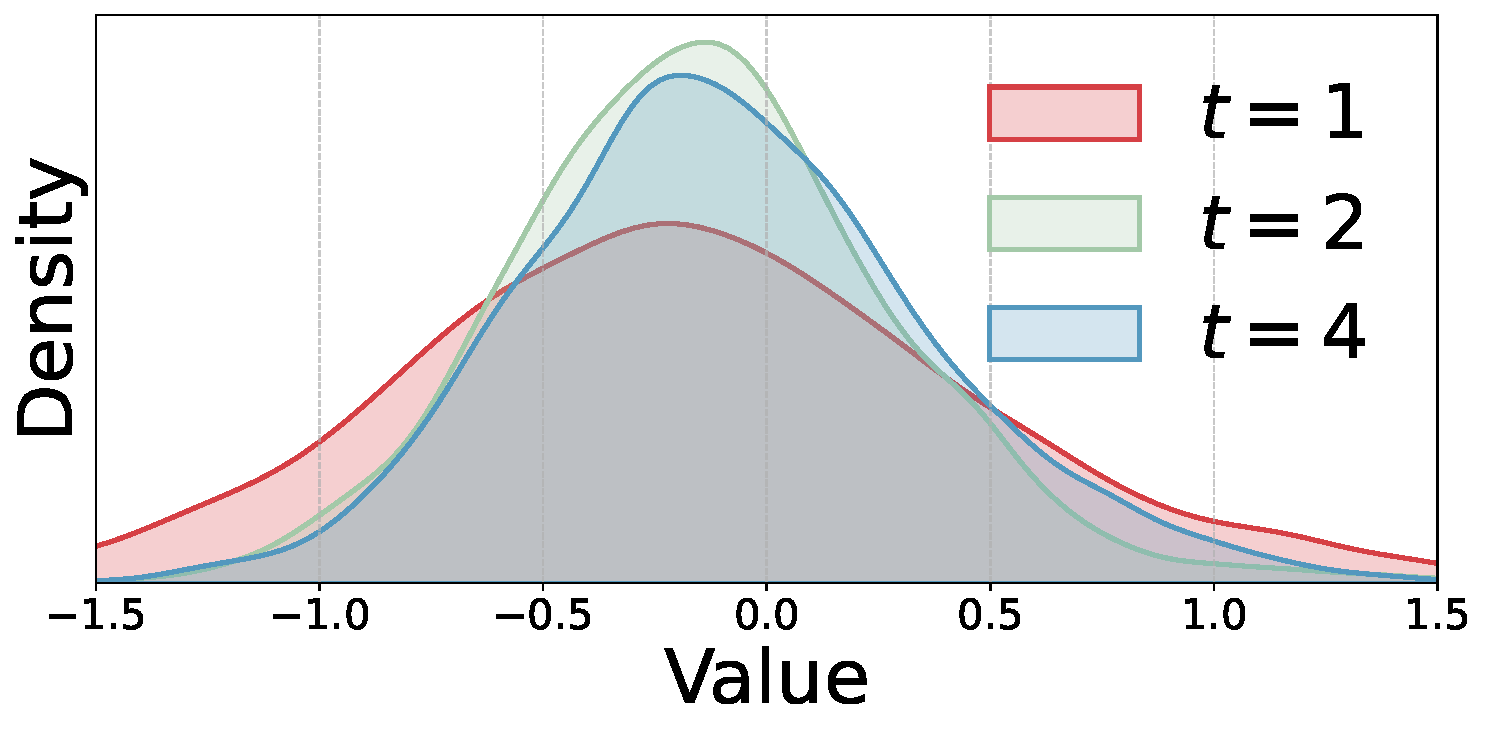
\includegraphics[width=0.95\linewidth]{fig/density_plot_presynaptic_input_tab.pdf}
    \caption{TAB}
  \end{subfigure}
  \hfill
  \begin{subfigure}{0.495\linewidth}
    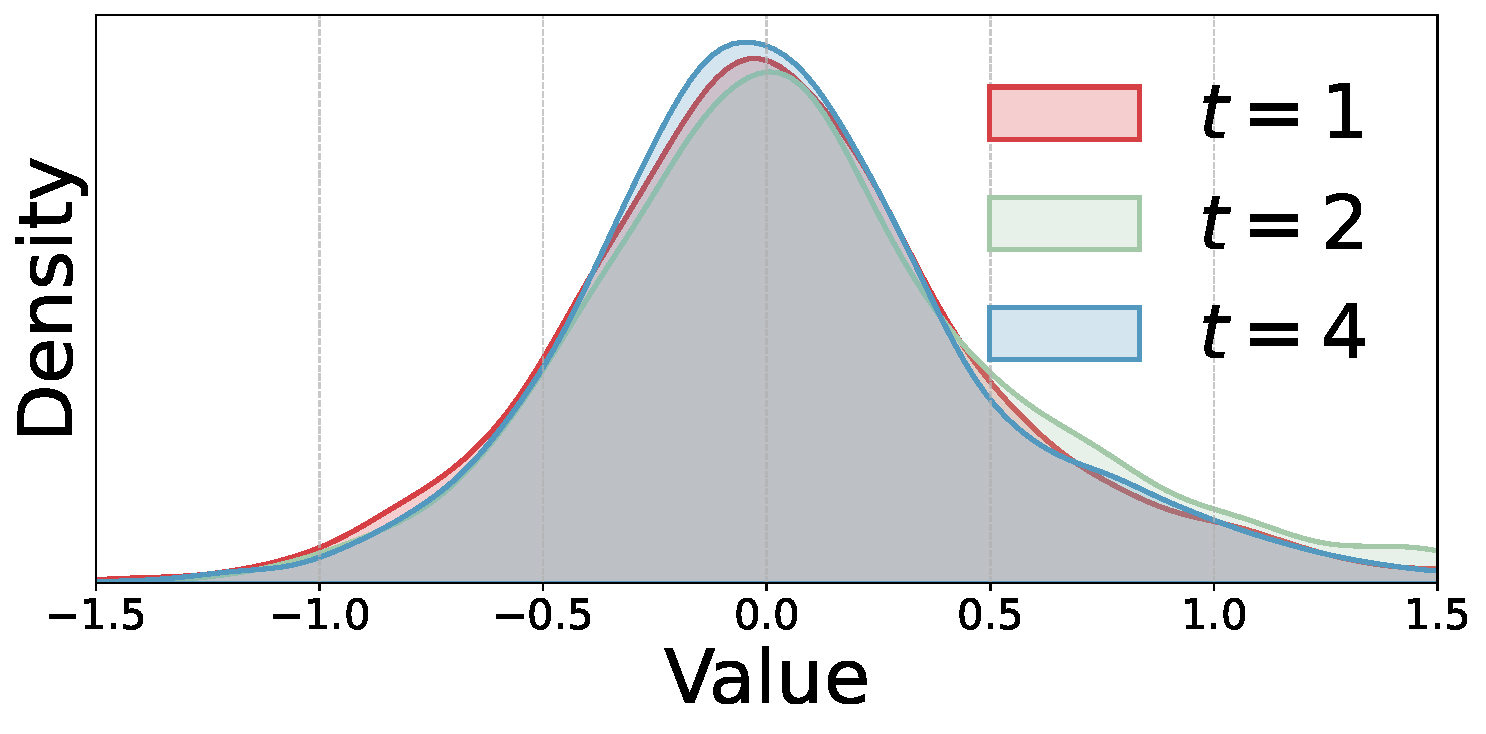
\includegraphics[width=0.95\linewidth]{fig/density_plot_presynaptic_input_mpinit.pdf}
    \caption{MP-Init (ours)}
  \end{subfigure}
  \caption{Activation (presynaptic input) distributions of the convolutional layer following the third spiking layer of ResNet-19 on CIFAR-100. The drift visible in TEBN and TAB collapses under MP-Init.}
  \label{fig:combined_activation}
\end{figure}

\section{Root Cause of TCS}
\label{sec:mpinit_root}

We claim that TCS in activations fundamentally originates from TCS in the membrane potential. By \cref{eq:lif_discrete_firing}, the spike output depends directly on the membrane potential; if the membrane potential drifts significantly over timesteps, the activation distribution shifts correspondingly.

\Cref{fig:combined_membrane} visualizes the membrane potential at each timestep and validates this claim. tdBN, which does not account for TCS, exhibits a clear temporal drift, leading to TCS in the activation distribution (\cref{fig:combined_activation}). While TEBN and TAB attempt to stabilize activations through timestep-dependent normalization, the membrane potential itself continues to drift, preserving TCS in activations.

\section{Convergence of the Membrane Potential}
\label{sec:mpinit_theorem}

While the empirical evidence above demonstrates the existence of TCS in the membrane potential, a theoretical perspective provides a deeper understanding. In this section we present the core principles explaining \emph{why} the membrane potential drifts.

We prove that the layer-wise distribution of the membrane potential converges to a (possibly non-trivial) stationary distribution. The continuous-time analogue was previously established for stable input statistics~\cite{dumont:2017}; we extend the result to the discrete-time model and show that the same convergence property holds.

\begin{assumption}[i.i.d.\ inputs and bounded membrane potential]
\label{assum:1}
Let $\{I_{\text{in}}[t]\}_{t\ge1}$ be a sequence drawn from an i.i.d.\ distribution. Furthermore, suppose there exist real constants $u^- < u^+$ such that the membrane potential $U[t]$ of active neurons in each layer remains within $[u^-, u^+]$ for all $t$.
\end{assumption}

The i.i.d.\ assumption is reasonable: inputs $\{I_{\text{in}}[t]\}_{t\ge1}$ are drawn repeatedly from a dataset or from a normalized layer. While soft-reset LIF dynamics do not strictly prevent unbounded growth, well-trained SNNs rarely exhibit it in active neurons. An empirical validation of \cref{assum:1} is provided in \cref{sec:mpinit_validation}.

\begin{theorem}[Geometric convergence to a stationary distribution]
\label{thm:1}
Under \cref{assum:1}, the sequence $\{U[t]\}_{t \ge 0}$ forms a Markov chain with transition kernel $P$. This chain satisfies Doeblin's minorization condition, and consequently admits a unique stationary distribution $\pi$. Moreover, the total-variation (TV) distance between $U[t]$ and $\pi$ decreases exponentially fast in $t$.
\end{theorem}

\begin{proof}
The proof proceeds in four steps: (Step 1) verify the Markov property; (Step 2) characterize the transition kernel; (Step 3) establish Doeblin's minorization condition~\cite{rosenthal:1995}; and (Step 4) derive exponential decay in TV distance.

\medskip
\noindent\textbf{Step 1: Markov property.}
The dynamics of $U[t]$ are
\begin{equation}
    U[t+1] \;=\; f\!\bigl(U[t],\,I_{\text{in}}[t+1]\bigr),
\end{equation}
where $f(\cdot)$ is a deterministic function of the current membrane potential $U[t]$ and the new input $I_{\text{in}}[t+1]$. Since $\{I_{\text{in}}[t]\}_{t\ge1}$ is i.i.d., the future state $U[t+1]$ depends solely on the current state $U[t]$ and not on earlier states:
\begin{equation}
    \Pr\bigl(U[t+1]\in A \,\big|\, U[t],\dots,U[0]\bigr)
    \;=\;
    \Pr\bigl(U[t+1]\in A \,\big|\, U[t]\bigr).
\end{equation}
Hence $\{U[t]\}_{t\ge0}$ is a Markov chain.

\medskip
\noindent\textbf{Step 2: Transition kernel.}
The transition kernel $P(x,A)$ is the probability that $U[t+1]$ falls in the measurable set $A$ given $U[t]=x$:
\begin{equation}
    P(x,A) \;=\; \Pr\bigl(U[t+1]\in A \,\big|\, U[t]=x\bigr)
    \;=\; \int_{A} p(x,y)\,\mathrm{d}y,
\end{equation}
where the transition density $p(x,y)$ encapsulates the dynamics induced by $f(\cdot)$ and the i.i.d.\ input distribution.

\medskip
\noindent\textbf{Step 3: Doeblin's minorization condition.}
We show that there exist a constant $\epsilon>0$ and a probability measure $\mu(\cdot)$ on the state space $S=[u^{-},u^{+}]$ such that
\begin{equation}
\label{eq:minimorization_condition}
    P(x,A) \;\ge\; \epsilon\,\mu(A)
    \qquad \forall\, x\in S,\;\forall\, A\subseteq S \text{ measurable.}
\end{equation}
Because $S$ is bounded by \cref{assum:1} and the transition density $p(x,y)$ is continuous (the i.i.d.\ inputs ensure a smooth density on $S$), there exists a positive lower bound $\delta>0$ such that $p(x,y)\ge\delta$ for all $(x,y)\in S\times S$. Hence
\begin{equation}
    P(x,A) \;=\; \int_{A} p(x,y)\,\mathrm{d}y \;\ge\; \delta\cdot \lambda(A),
\end{equation}
where $\lambda$ is the Lebesgue measure on $S$. Letting $\mu(A)=\lambda(A)/\lambda(S)$ be the uniform probability measure on $S$ and $\epsilon=\delta\,\lambda(S)$ yields \cref{eq:minimorization_condition}.

\medskip
\noindent\textbf{Step 4: Exponential decay of TV distance.}
A direct consequence of Doeblin's minorization condition (see, e.g., \cite{rosenthal:1995}) is that the $n$-step transition $P^{n}(x,\cdot)$ converges geometrically to a unique stationary distribution $\pi$:
\begin{equation}
\label{eq:convergence_speed}
    \bigl\|P^{n}(x,\cdot)-\pi(\cdot)\bigr\|_{\mathrm{TV}} \;\le\; C\,(1-\epsilon)^{n}
\end{equation}
for some constant $C>0$ depending on the initial state. Since $1-\epsilon<1$, the TV distance decreases exponentially in $n$, simultaneously establishing the existence and uniqueness of the stationary distribution.
\end{proof}

\Cref{thm:1} indicates that TCS in the membrane potential is \emph{inevitable} whenever the initial membrane potential differs from its stationary distribution. Traditionally the membrane potential is initialized to zero, $U[0]=0$; this zero initialization is a primary contributor to TCS. To mitigate TCS, we therefore must reduce the discrepancy between the initial state and the stationary distribution.

\section{Optimal Constant Initialization}
\label{sec:mpinit_lemma}

Theorem~\ref{thm:1} implies that eliminating the mismatch between the initial state and the stationary distribution is crucial. Directly computing $\pi$ is intractable; we therefore propose a more practical approach—initialize the membrane potential with a \emph{per-layer constant} that approximates the mean of $\pi$.

\begin{lemma}[Mean optimality among constants]
\label{lemma:1}
Let $U^{*}\sim \pi$ be a sample from the stationary distribution. Among all constants $c \in \mathbb{R}$, the choice $c = \mathbb{E}[U^{*}]$ minimizes the expected square difference $\mathbb{E}[(U^{*}-c)^{2}]$.
\end{lemma}

\begin{proof}
Expanding the square,
\begin{equation}
    \mathbb{E}[(U^{*}-c)^{2}] \;=\; \mathbb{E}[U^{*2}] - 2\,\mathbb{E}[U^{*}]\,c + c^{2}.
\end{equation}
Differentiating with respect to $c$ and setting the derivative to zero,
\begin{equation}
    \frac{\partial \mathbb{E}[(U^{*}-c)^{2}]}{\partial c} \;=\; -2\,\mathbb{E}[U^{*}] + 2c \;=\; 0
    \quad\Longrightarrow\quad
    c \;=\; \mathbb{E}[U^{*}].
\end{equation}
The second derivative is $2>0$, confirming that the critical point is a minimum.
\end{proof}

\Cref{lemma:1} suggests that initializing the membrane potential to the stationary mean is optimal for eliminating drift while minimizing variance. The remaining challenge is to approximate $\mathbb{E}[\pi]$ in practice.

A simple solution leverages \cref{thm:1}: a membrane-potential distribution converges exponentially to $\pi$, so the membrane potential at the final timestep $U[T]$ is the closest sample to $\pi$. We therefore approximate the per-layer statistic of $\mathbb{E}[\pi]$ using $\mathbb{E}[U[T]]$.

\section{The MP-Init Algorithm}
\label{sec:mpinit_algorithm}

To implement the idea efficiently, we compute the average membrane potential $U[T]$ at the final timestep for each layer during training. This average is used to update a running mean $r$, initialized to zero at the beginning of training. Before feeding each batch into the network—both during training and at inference—we initialize the membrane potential of every layer to this running mean, $U[0] = r$. The procedure, called \textbf{MP-Init}, requires negligible extra memory or computation. \Cref{alg:mpinit} summarizes the steps.

\begin{algorithm}[h]
\caption{MP-Init: per-layer running-mean initialization}
\label{alg:mpinit}
\begin{algorithmic}[1]
\State Initialize per-layer running mean $\mu^{l}\!\leftarrow\!0$ for each layer $l$
\State \textbf{Training phase:}
\For{each batch with simulation window of length $T$}
  \State Set initial membrane potential $U^{l}[0] \leftarrow \mu^{l}$
  \State Initialize activity mask $\texttt{mask}^{l}\leftarrow 0$
  \For{$t=1$ to $T$}
    \State Update $M^{l}[t]$ via \cref{eq:lif_discrete_potential}
    \State Compute spikes $S^{l}[t]$ via \cref{eq:lif_discrete_firing}
    \State Reset $U^{l}[t]$ via \cref{eq:lif_discrete_reset}
    \State $\texttt{mask}^{l}\leftarrow \texttt{mask}^{l}\;\textsc{or}\;(S^{l}[t]>0)$
  \EndFor
  \State $\bar{U}^{l}\leftarrow \mathrm{mean}\{U^{l}[T] : \texttt{mask}^{l}=1\}$ \Comment{active neurons only}
  \State $\mu^{l}\leftarrow \beta\,\mu^{l} + (1-\beta)\,\bar{U}^{l}$ \Comment{EMA update, $\beta=0.9$}
\EndFor
\State \textbf{Inference phase:} keep $\mu^{l}$ fixed; initialize $U^{l}[0]\leftarrow \mu^{l}$ at every batch.
\end{algorithmic}
\end{algorithm}

As illustrated in \cref{fig:combined_membrane,fig:combined_activation}, MP-Init effectively resolves both TCS in the membrane potential and TCS in activations, yielding consistent distributions across timesteps. Importantly, MP-Init is straightforward to implement, does not modify BN layers, and does not introduce complex training pipelines—unlike TEBN~\cite{tebn:2022} or TAB~\cite{tab:2024}. This simplicity significantly enhances usability across applications without altering existing recipes.

\section{Empirical Validation of \texorpdfstring{\Cref{assum:1}}{Assumption 1}}
\label{sec:mpinit_validation}

We provide three checks of \cref{assum:1} in our trained networks: (i) the i.i.d.\ behavior of presynaptic inputs, (ii) the boundedness of $U[t]$, and (iii) the geometric TV decay implied by \cref{thm:1}.

\paragraph{(i) Independence of inputs.}
We perform a Ljung--Box test at lag~1 on the per-timestep presynaptic-input statistics. The test fails to reject the null hypothesis of zero serial correlation in the vast majority of layers on both CIFAR-100 (\cref{fig:ljung_static}) and DVS-CIFAR10 (\cref{fig:ljung_dvs}), supporting the i.i.d.\ assumption.

\begin{figure}[h]
  \centering
  \begin{subfigure}{0.49\linewidth}
    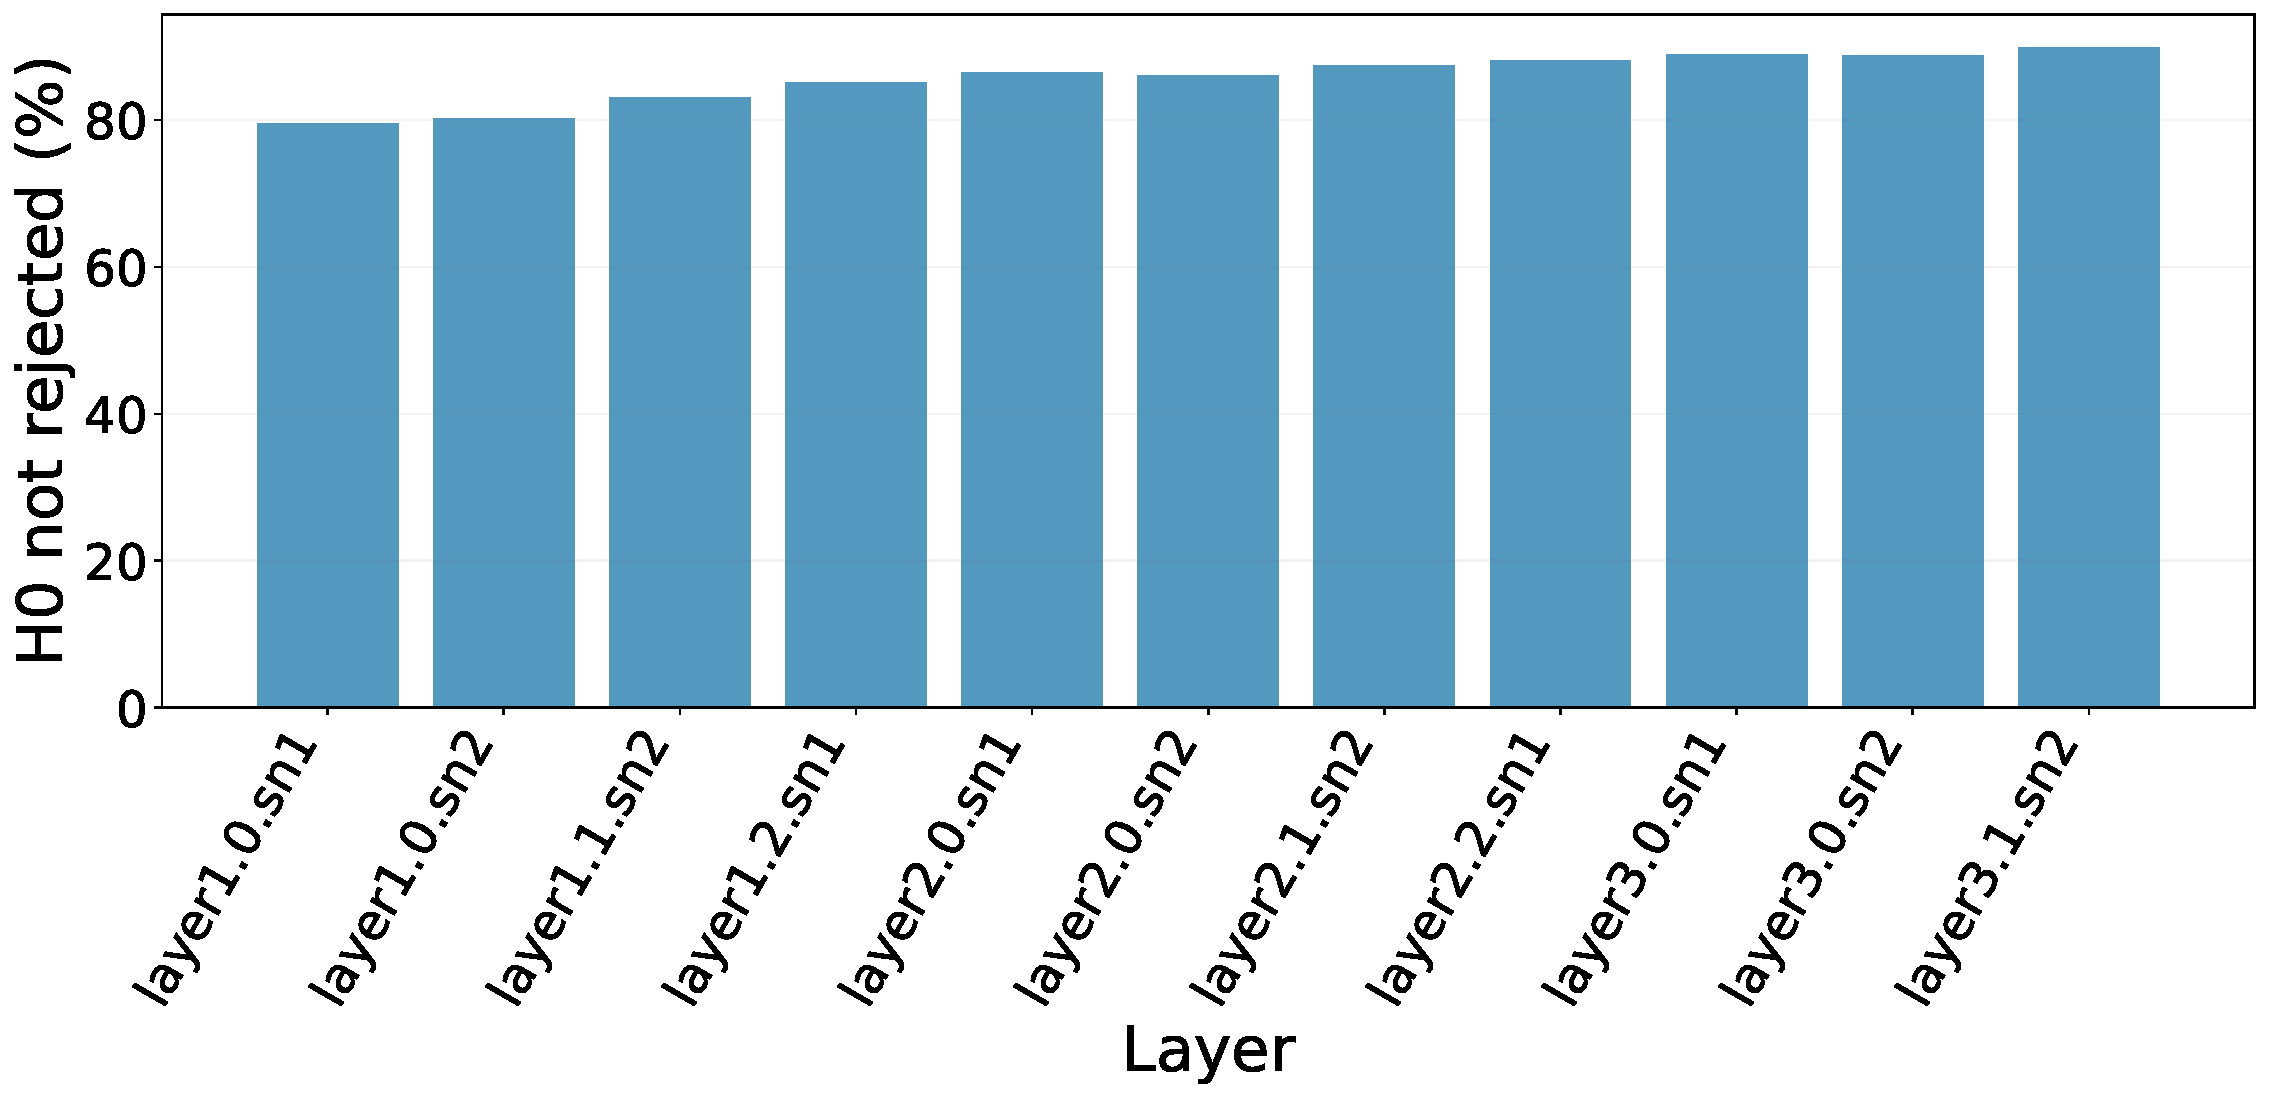
\includegraphics[width=\linewidth]{fig/ljung_box_lag1.pdf}
    \caption{CIFAR-100, ResNet-19}
    \label{fig:ljung_static}
  \end{subfigure}
  \hfill
  \begin{subfigure}{0.49\linewidth}
    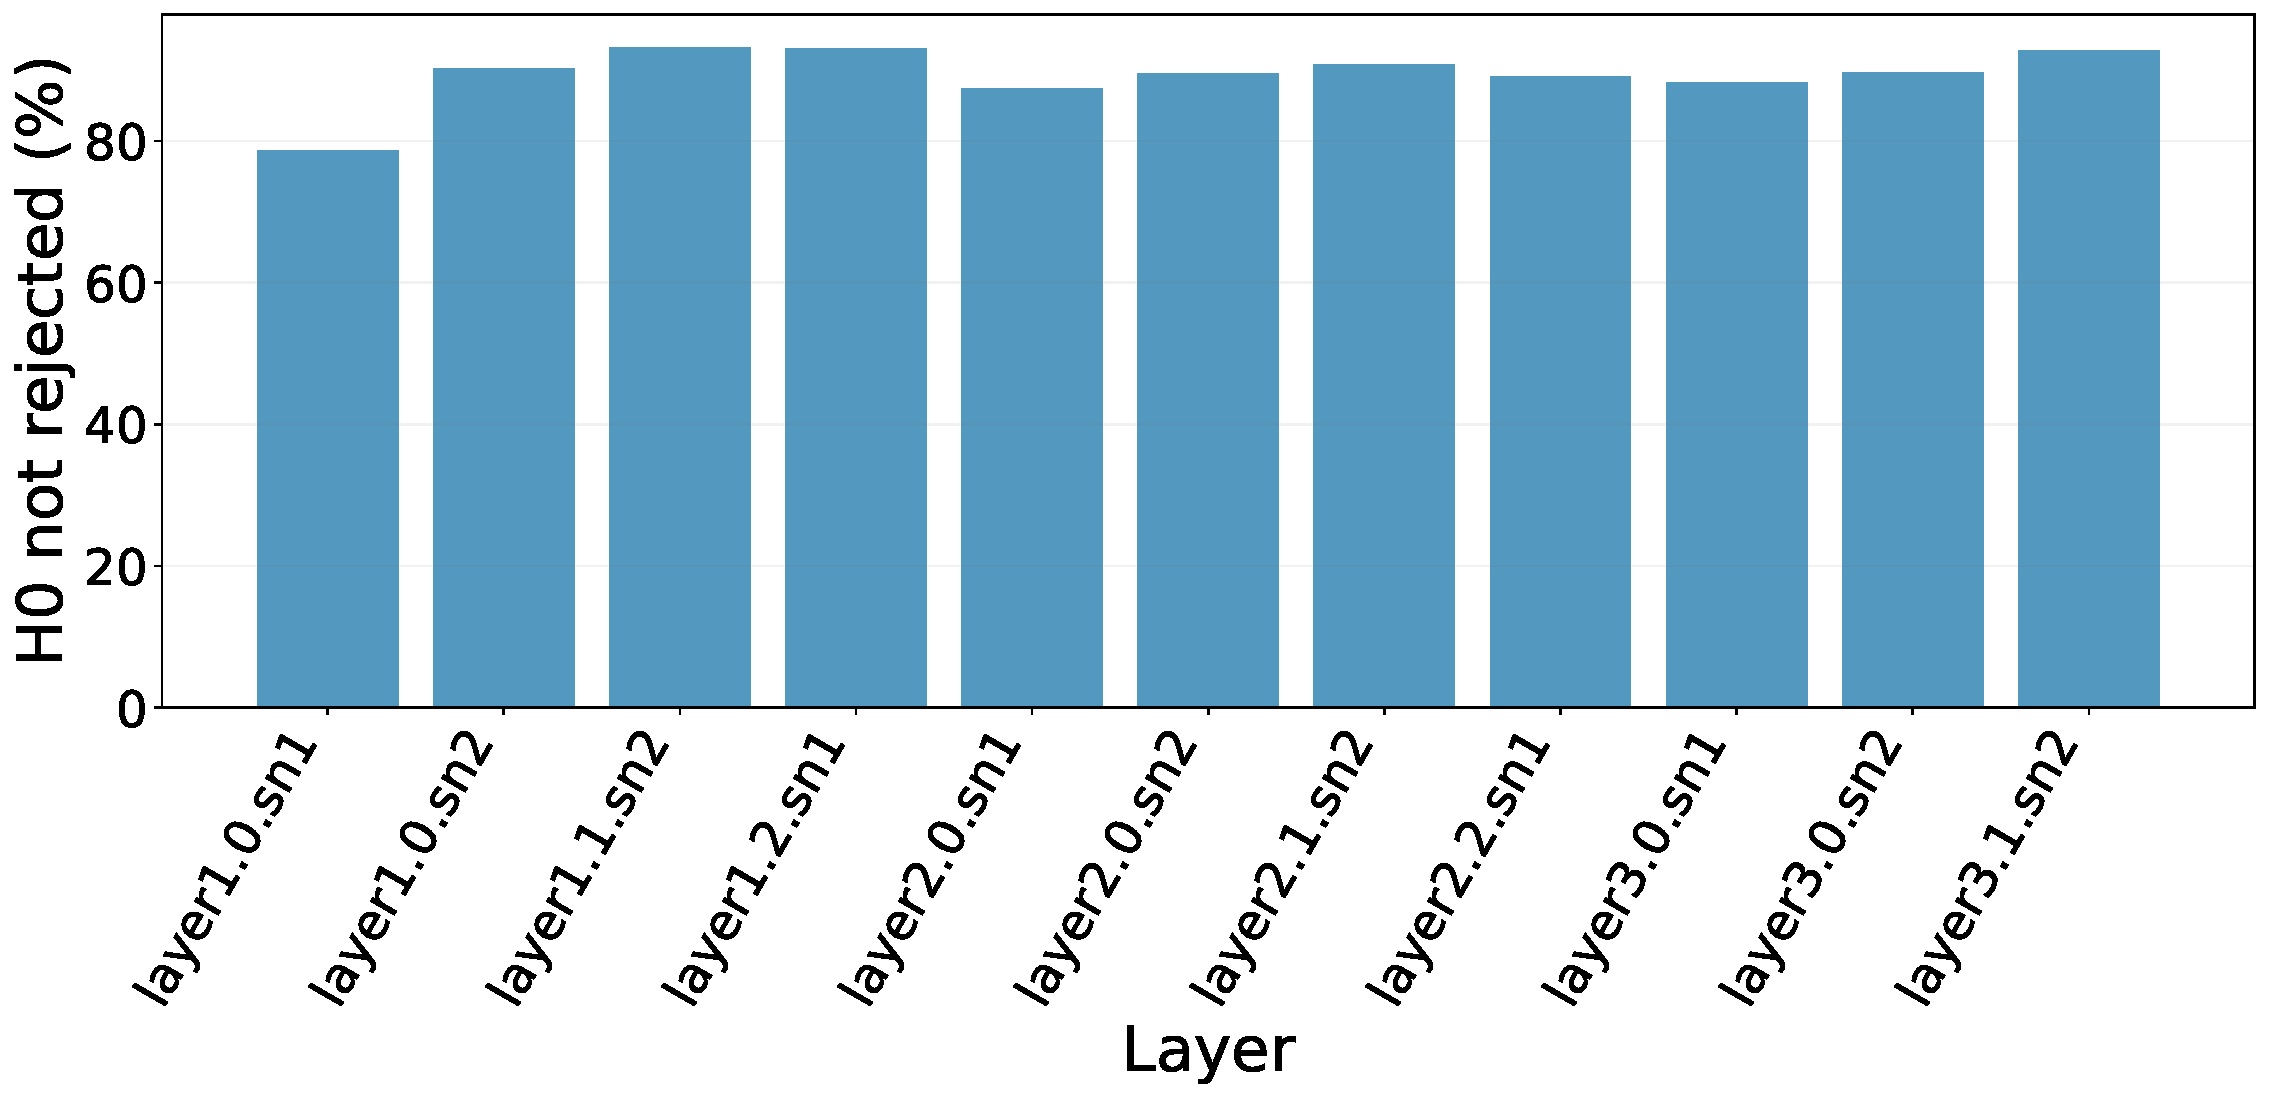
\includegraphics[width=\linewidth]{fig/ljung_box_lag1_dvs.pdf}
    \caption{DVS-CIFAR10, ResNet-19}
    \label{fig:ljung_dvs}
  \end{subfigure}
  \caption{Ljung--Box test (lag~1) for the presynaptic input across layers and timesteps.}
  \label{fig:ljung}
\end{figure}

\paragraph{(ii) Bounded membrane potential.}
We measure the empirical ratio of $|U^{l}[t]|$ to a per-layer bound across active neurons; \cref{fig:ratio_ut} shows that the ratio remains well within unity throughout training, validating the boundedness portion of \cref{assum:1}.

\begin{figure}[h]
  \centering
  \begin{subfigure}{0.49\linewidth}
    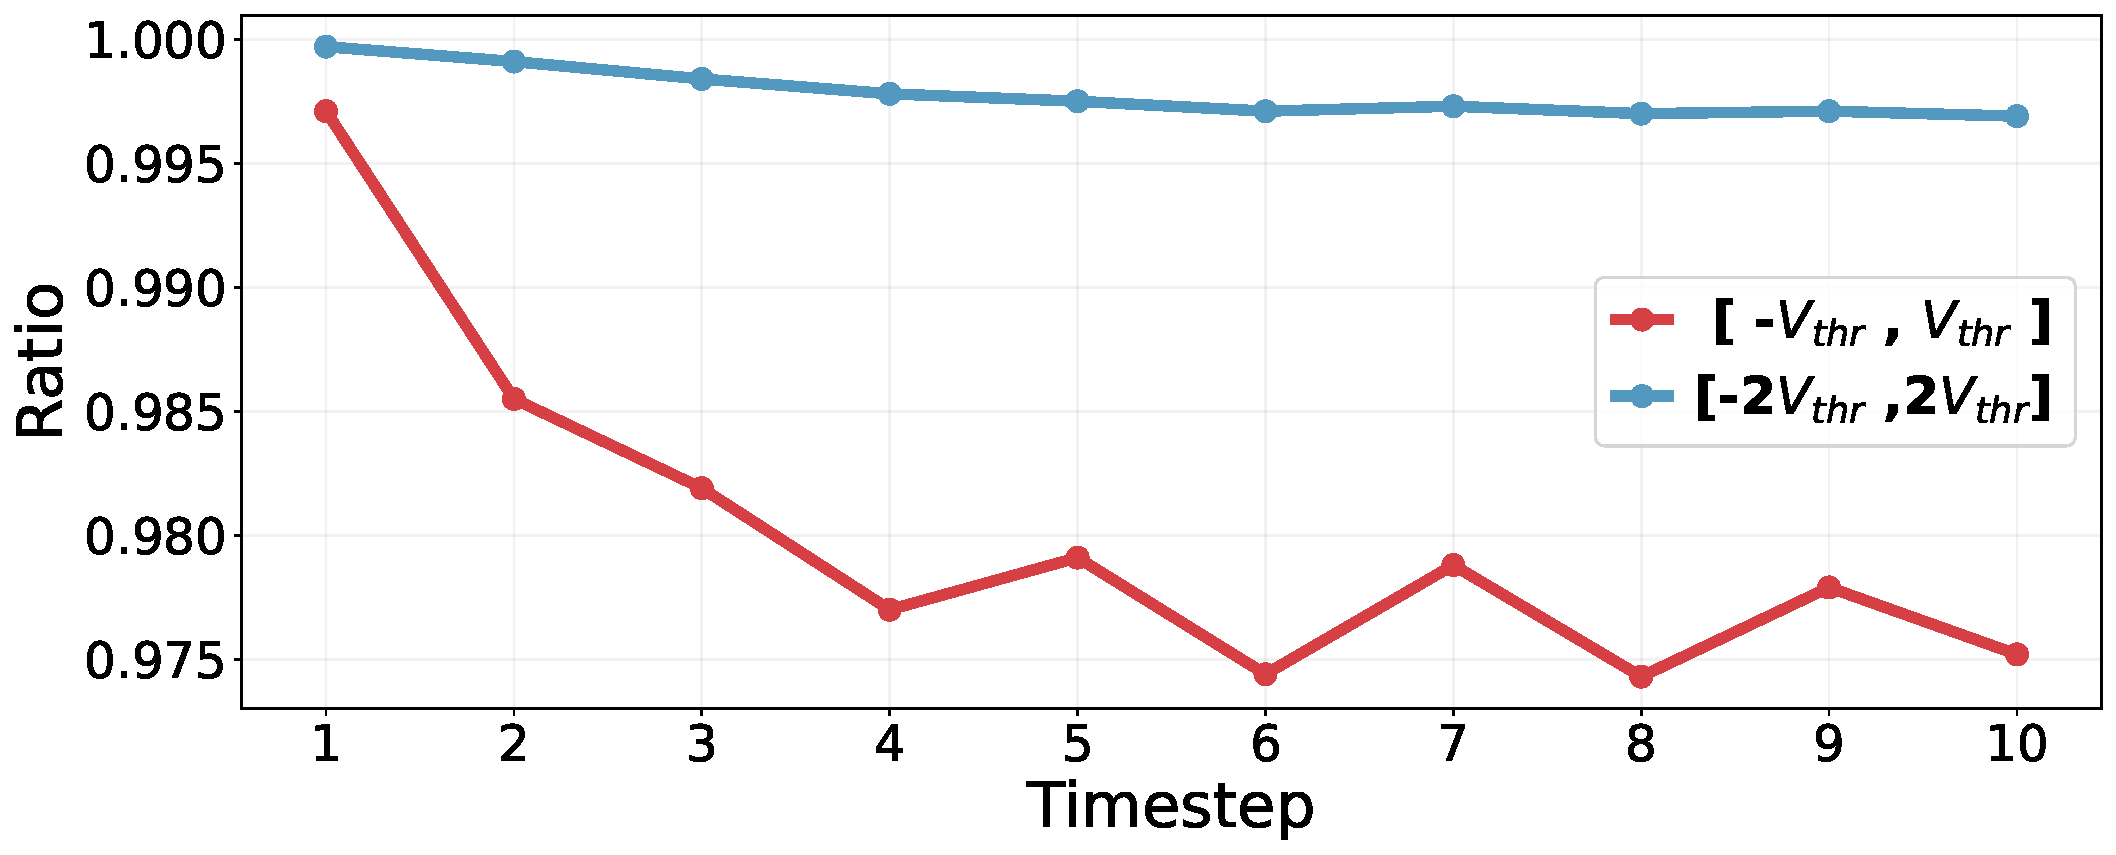
\includegraphics[width=\linewidth]{fig/ratio_ut.pdf}
    \caption{CIFAR-100}
  \end{subfigure}
  \hfill
  \begin{subfigure}{0.49\linewidth}
    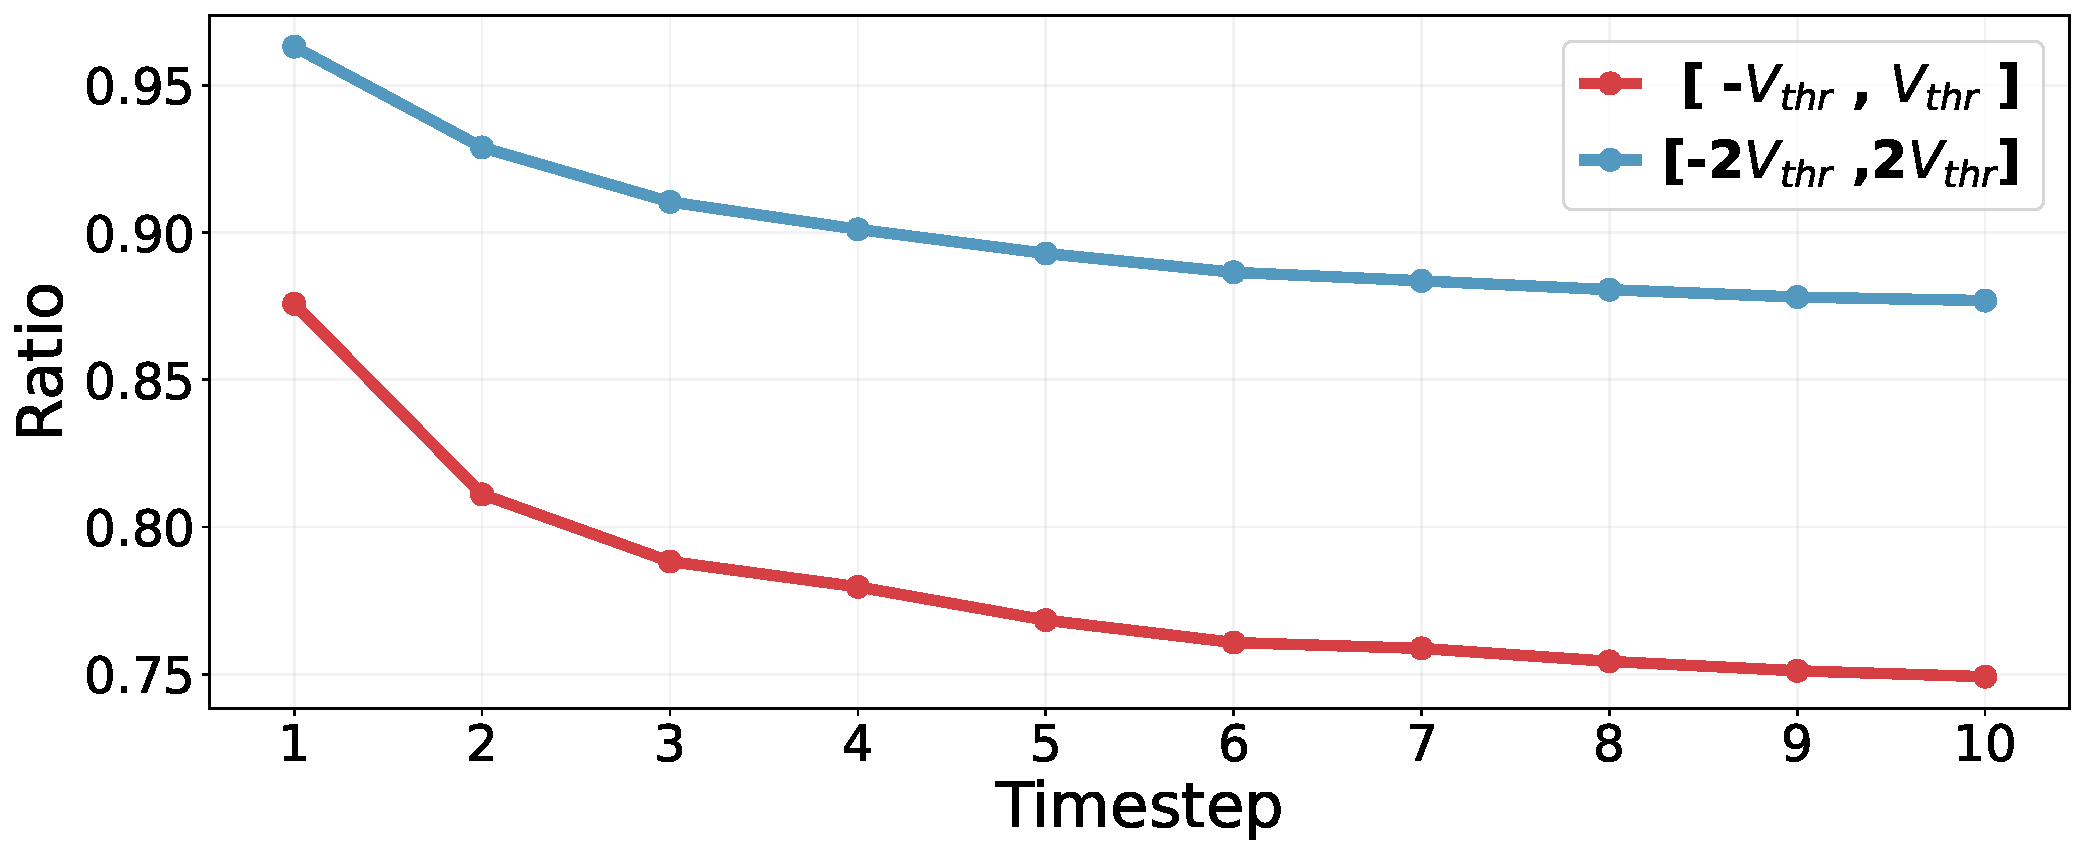
\includegraphics[width=\linewidth]{fig/ratio_ut_dvs.pdf}
    \caption{DVS-CIFAR10}
  \end{subfigure}
  \caption{Empirical bound on $|U^{l}[t]|$ for active neurons.}
  \label{fig:ratio_ut}
\end{figure}

\paragraph{(iii) Geometric TV decay.}
\Cref{fig:tv_decay} compares the empirical TV distance $\mathrm{TV}(U[t],\pi)$ as $t$ increases against an exponential reference. The decay is clearly geometric, in agreement with the conclusion of \cref{thm:1}.

\begin{figure}[h]
  \centering
  \begin{subfigure}{0.49\linewidth}
    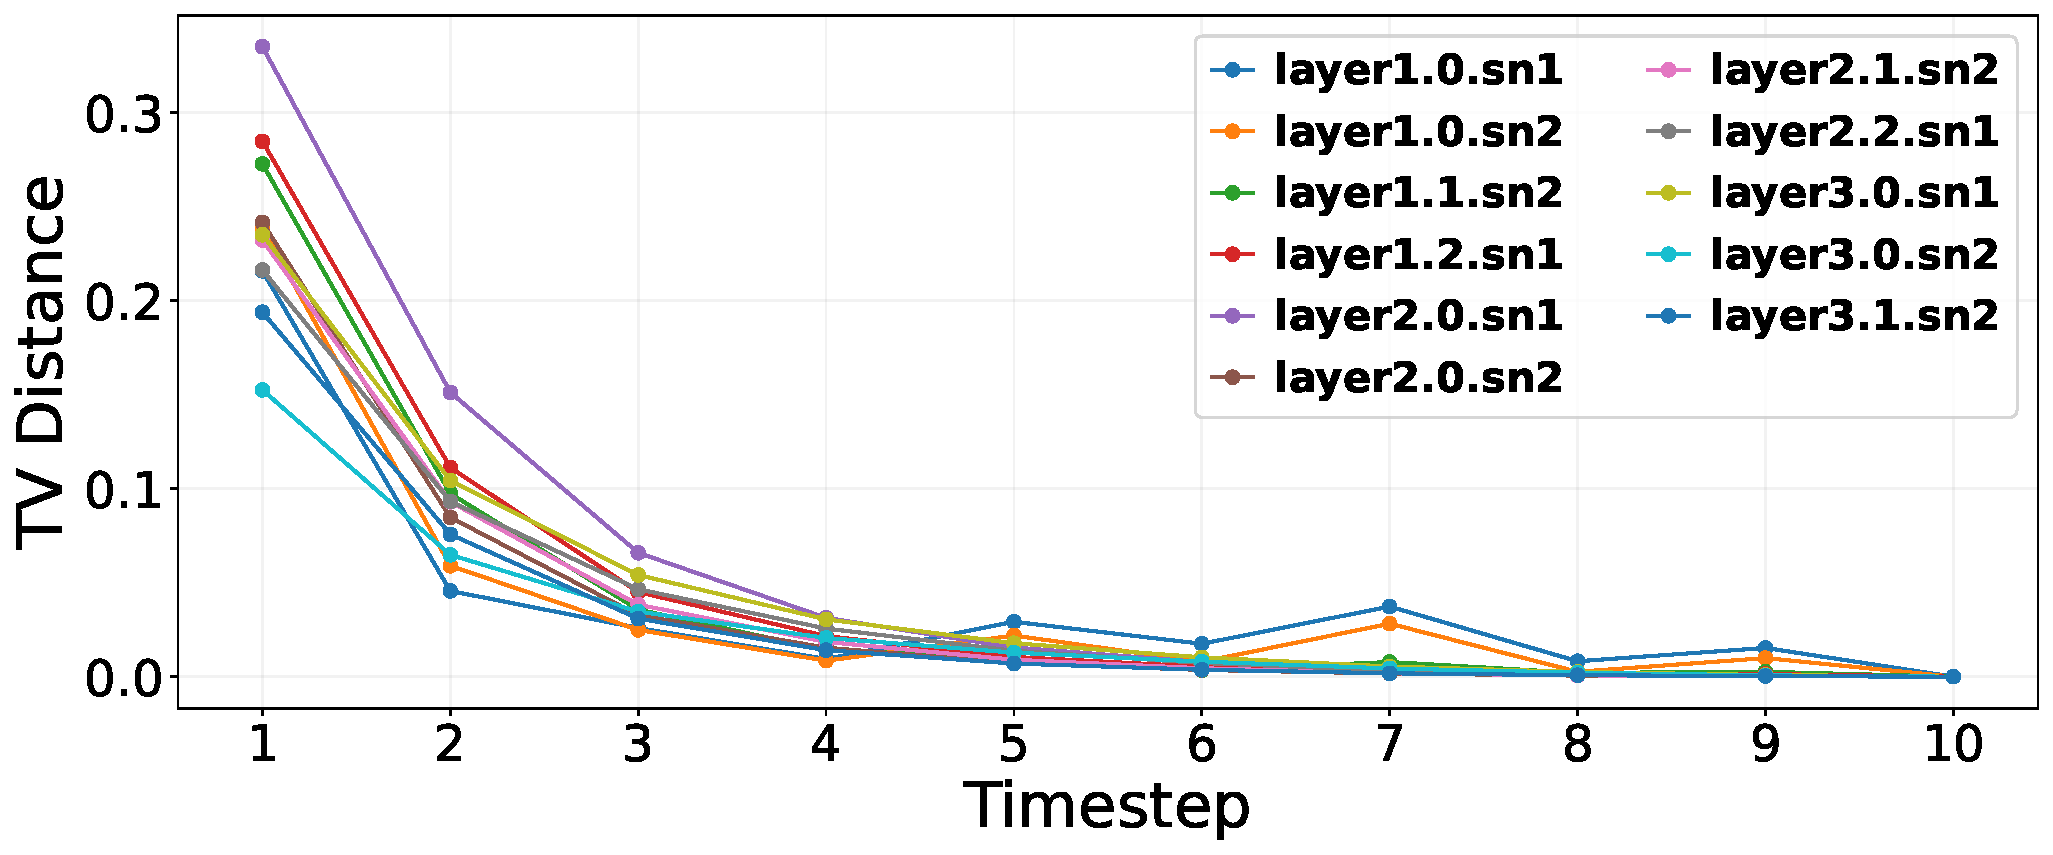
\includegraphics[width=\linewidth]{fig/tv_distance.pdf}
    \caption{CIFAR-100}
  \end{subfigure}
  \hfill
  \begin{subfigure}{0.49\linewidth}
    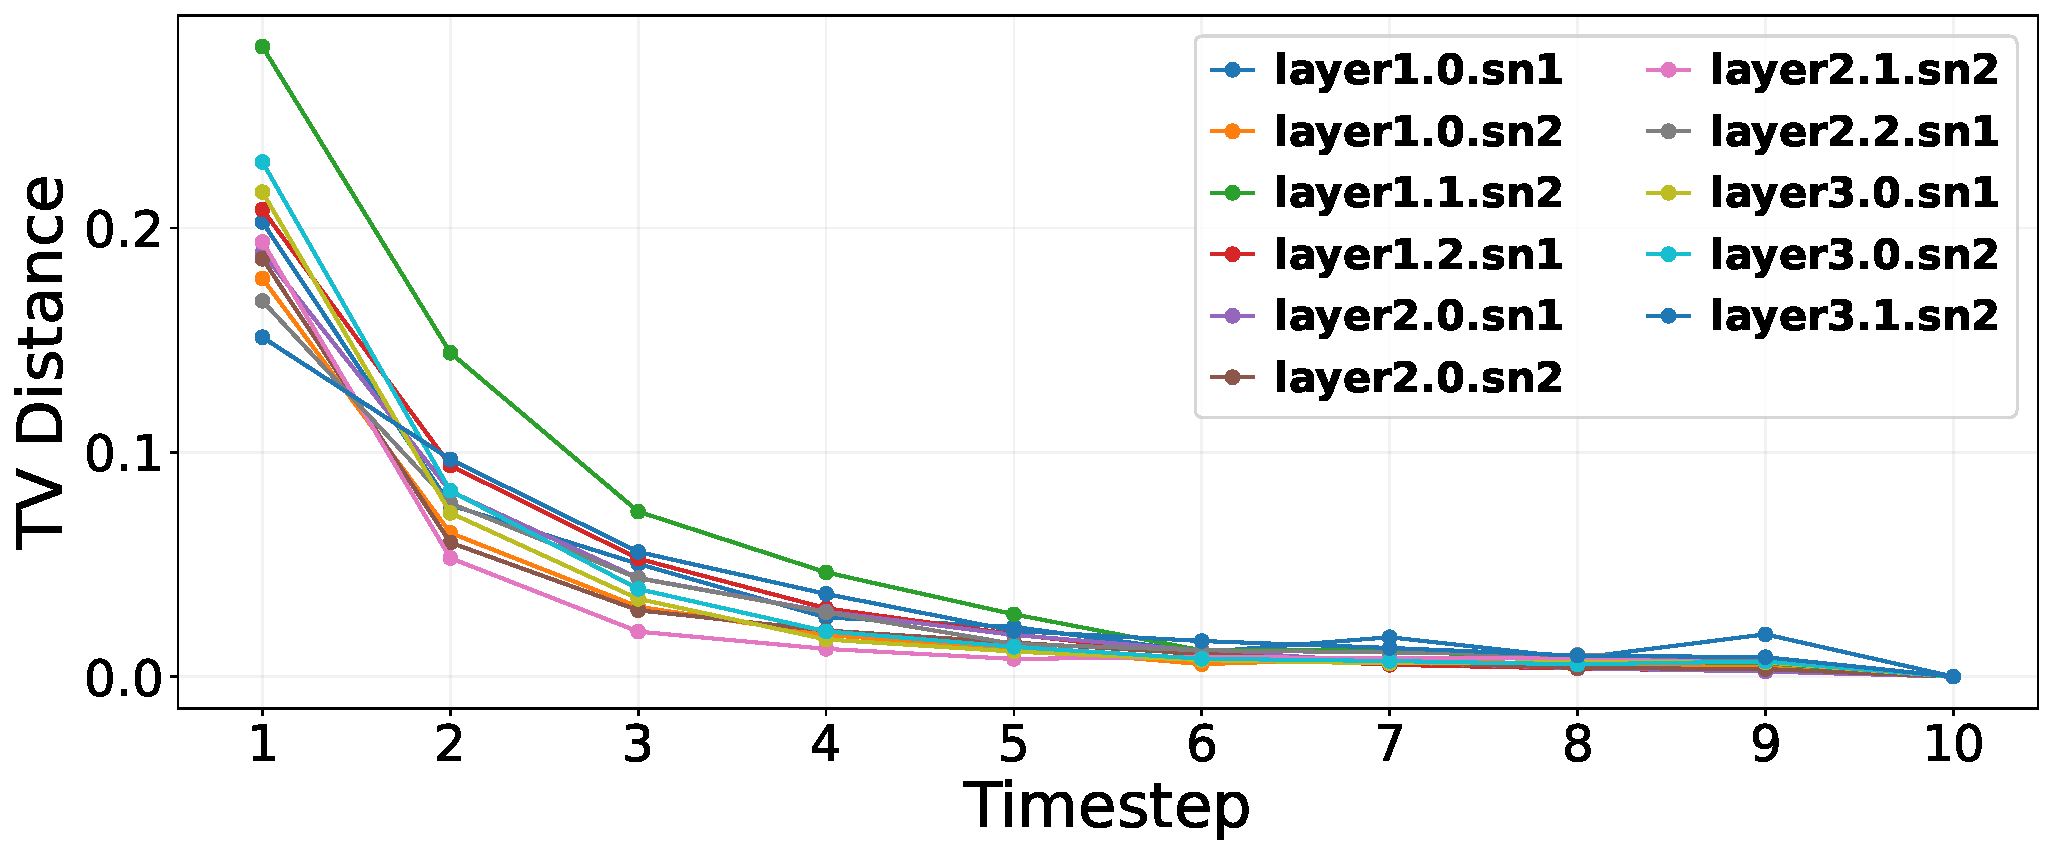
\includegraphics[width=\linewidth]{fig/tv_distance_dvs.pdf}
    \caption{DVS-CIFAR10}
  \end{subfigure}
  \caption{Total-variation distance between $U[t]$ and the stationary distribution $\pi$ as a function of $t$.}
  \label{fig:tv_decay}
\end{figure}

\begin{figure}[h]
  \centering
  \begin{subfigure}{0.49\linewidth}
    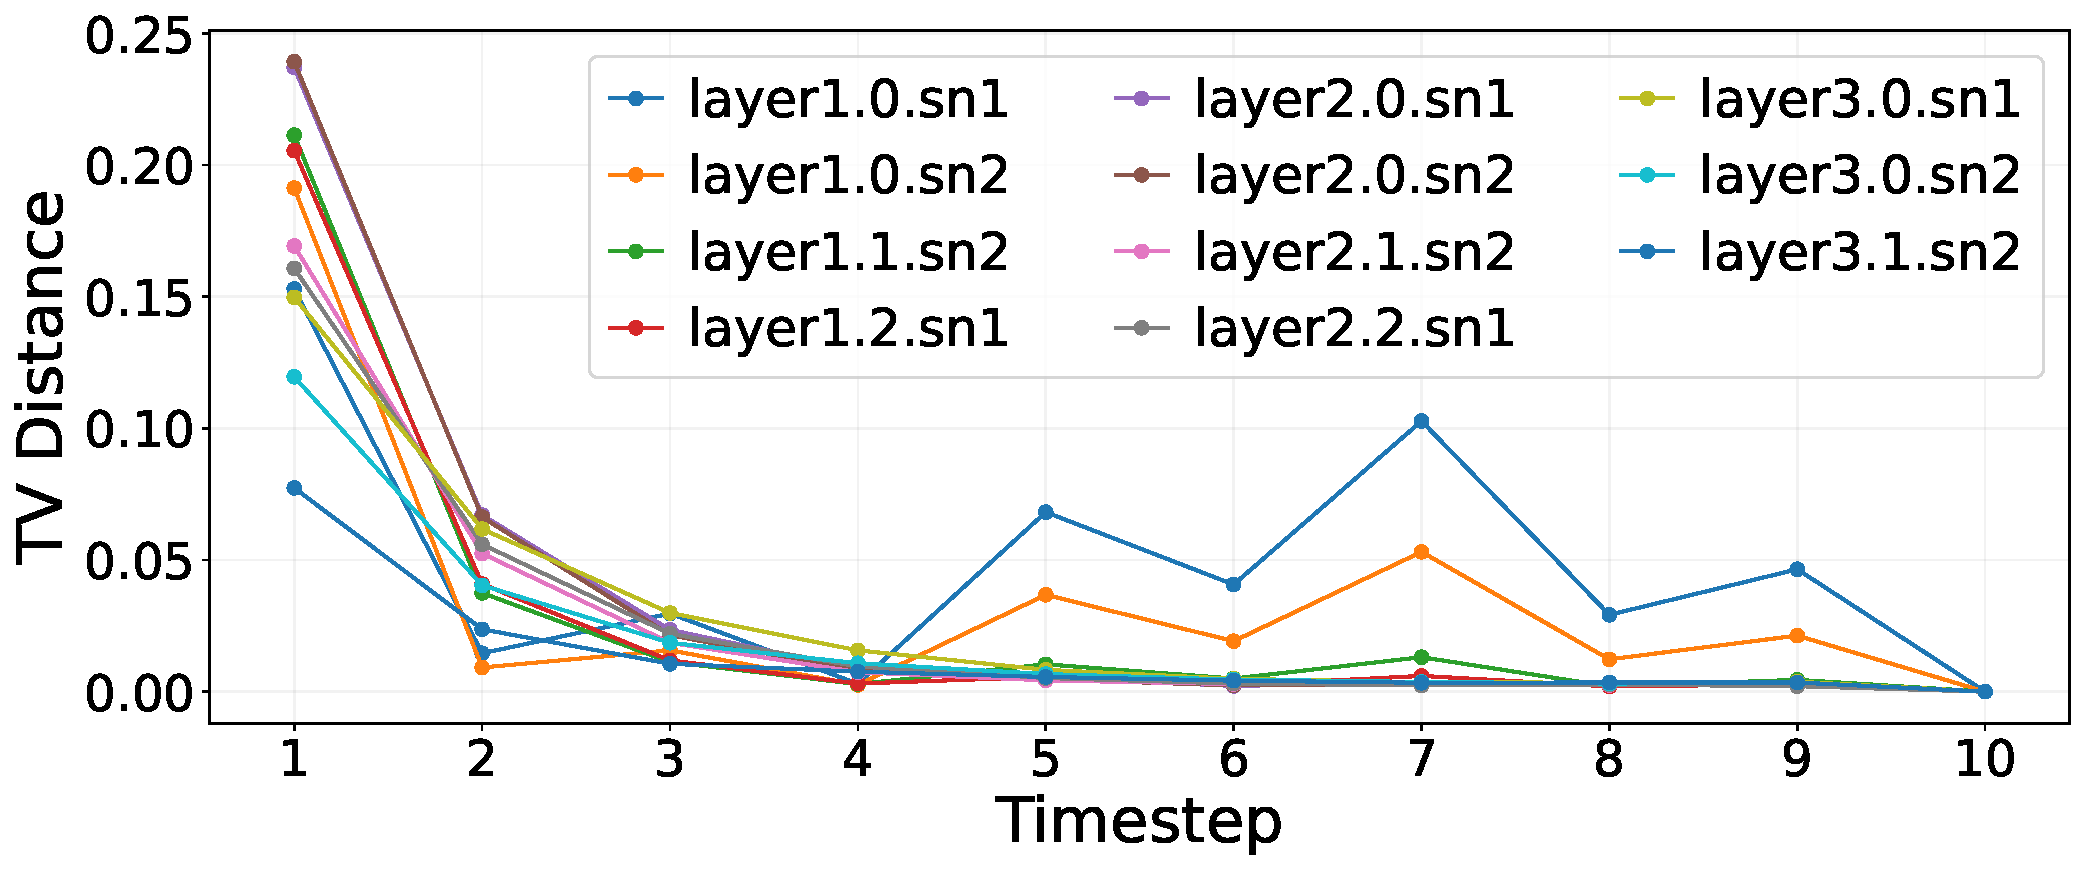
\includegraphics[width=\linewidth]{fig/tv_from_input_distribution.pdf}
    \caption{CIFAR-100}
  \end{subfigure}
  \hfill
  \begin{subfigure}{0.49\linewidth}
    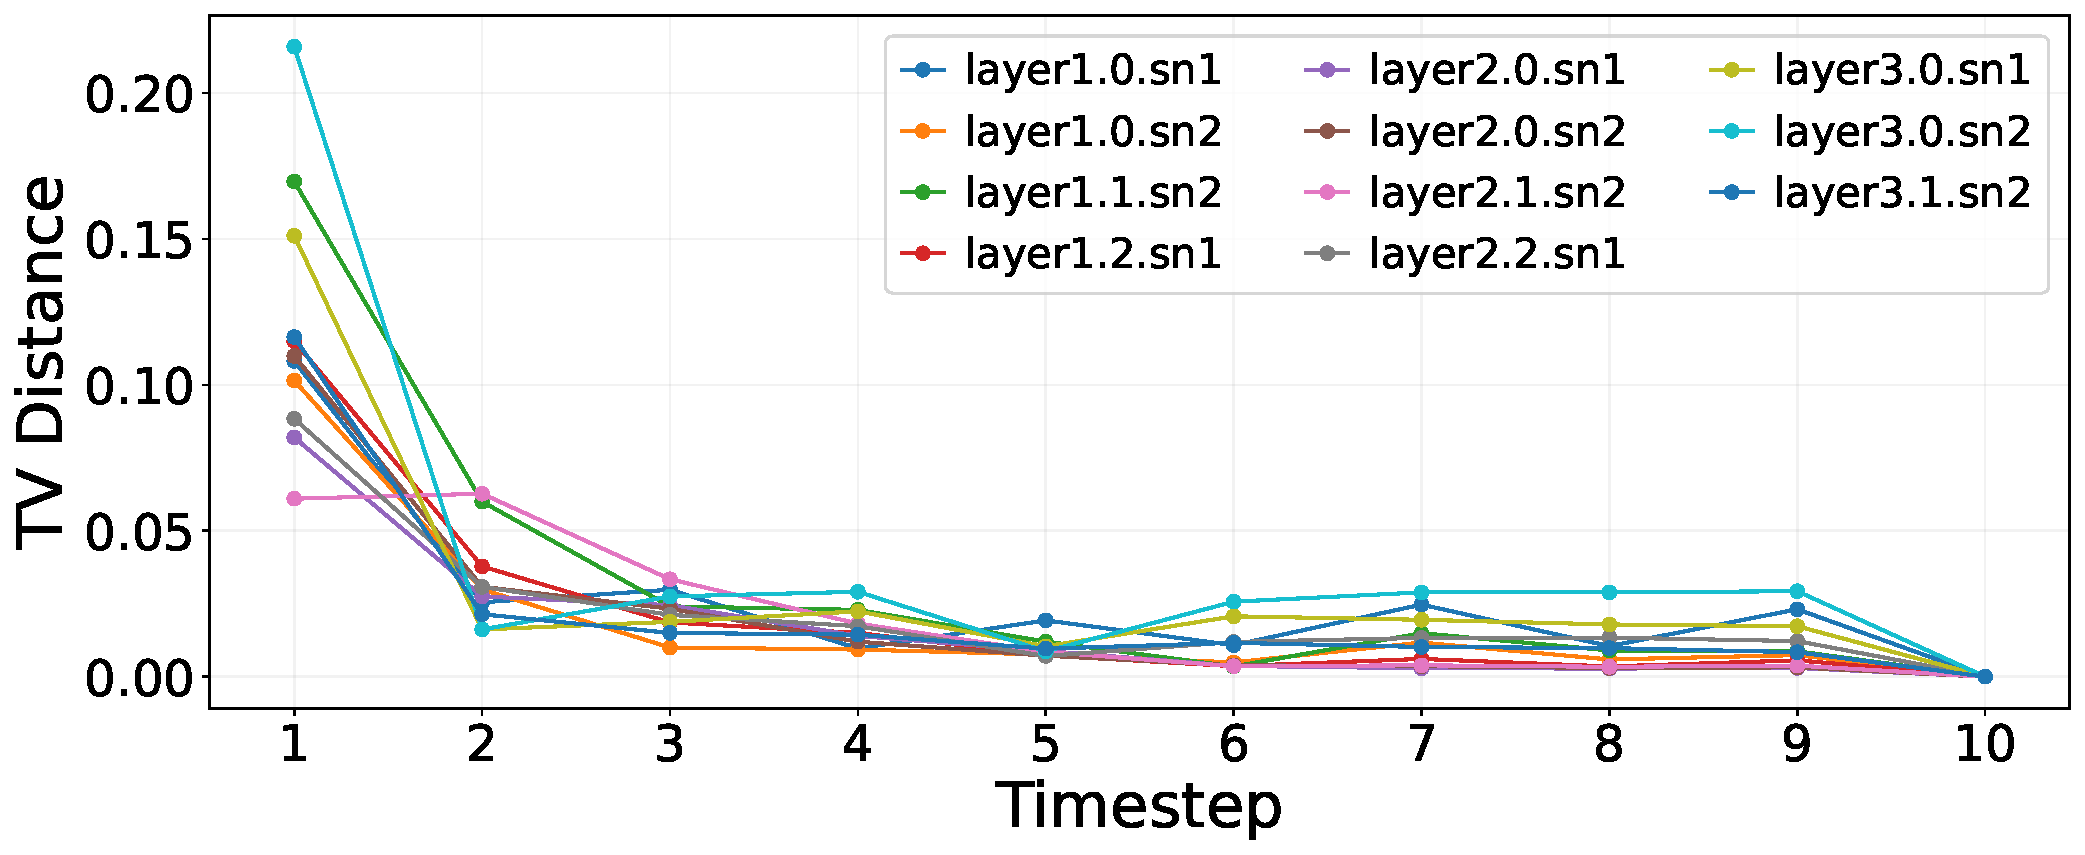
\includegraphics[width=\linewidth]{fig/tv_from_input_distribution_dvs.pdf}
    \caption{DVS-CIFAR10}
  \end{subfigure}
  \caption{TV distance from the input distribution as $t$ increases.}
  \label{fig:tv_input}
\end{figure}

\section{Biological Plausibility}
\label{sec:mpinit_bio}

A neuroscience study~\cite{yoo:2023} reports that resting membrane potentials (RMPs) differ across distinct cortical regions: neurons in the prefrontal cortex (PFC) exhibit $\sim 10$~mV higher RMPs than neurons in the posterior parietal cortex (PPC), driven by region-specific recurrent synaptic strengths mediated by NMDA receptors. These regional differences imply that the stationary membrane-potential distribution may inherently vary across neural populations and brain areas. The layer-wise initialization of MP-Init mirrors this intrinsic regional variability, lending biological plausibility to the proposed scheme.

\section{Summary}
\label{sec:mpinit_summary}

This chapter identified the membrane potential as the root cause of TCS in SNNs (\cref{sec:mpinit_root,sec:mpinit_empirical}), proved that the membrane potential converges geometrically to a stationary distribution (\cref{sec:mpinit_theorem}), and used this fact to derive a per-layer running-mean initialization, MP-Init, that eliminates TCS at negligible cost (\cref{sec:mpinit_algorithm}).

    \chapter{Threshold-Robust Surrogate Gradient (TrSG)}
\label{ch:trsg}

This chapter presents the second contribution of the thesis: \textbf{TrSG}, a surrogate-gradient (SG) formulation whose gradient magnitude is invariant to the threshold scale and whose active region adapts naturally with $V_{\text{thr}}$. \Cref{sec:trsg_background} reviews surrogate-gradient descent. \Cref{sec:trsg_two_families} dissects two existing families—Absolute-Scale (AS-SG) and Relative-Scale (RS-SG)—and shows how each becomes unstable when $V_{\text{thr}}$ is trainable. \Cref{sec:trsg_method} derives TrSG, and \Cref{sec:trsg_grad_analysis,sec:trsg_compatibility} provide a detailed gradient analysis with respect to $V_{\text{thr}}$ and $\tau$ together with compatibility checks across surrogate shapes.

\begin{figure}[t!]
    \centering
    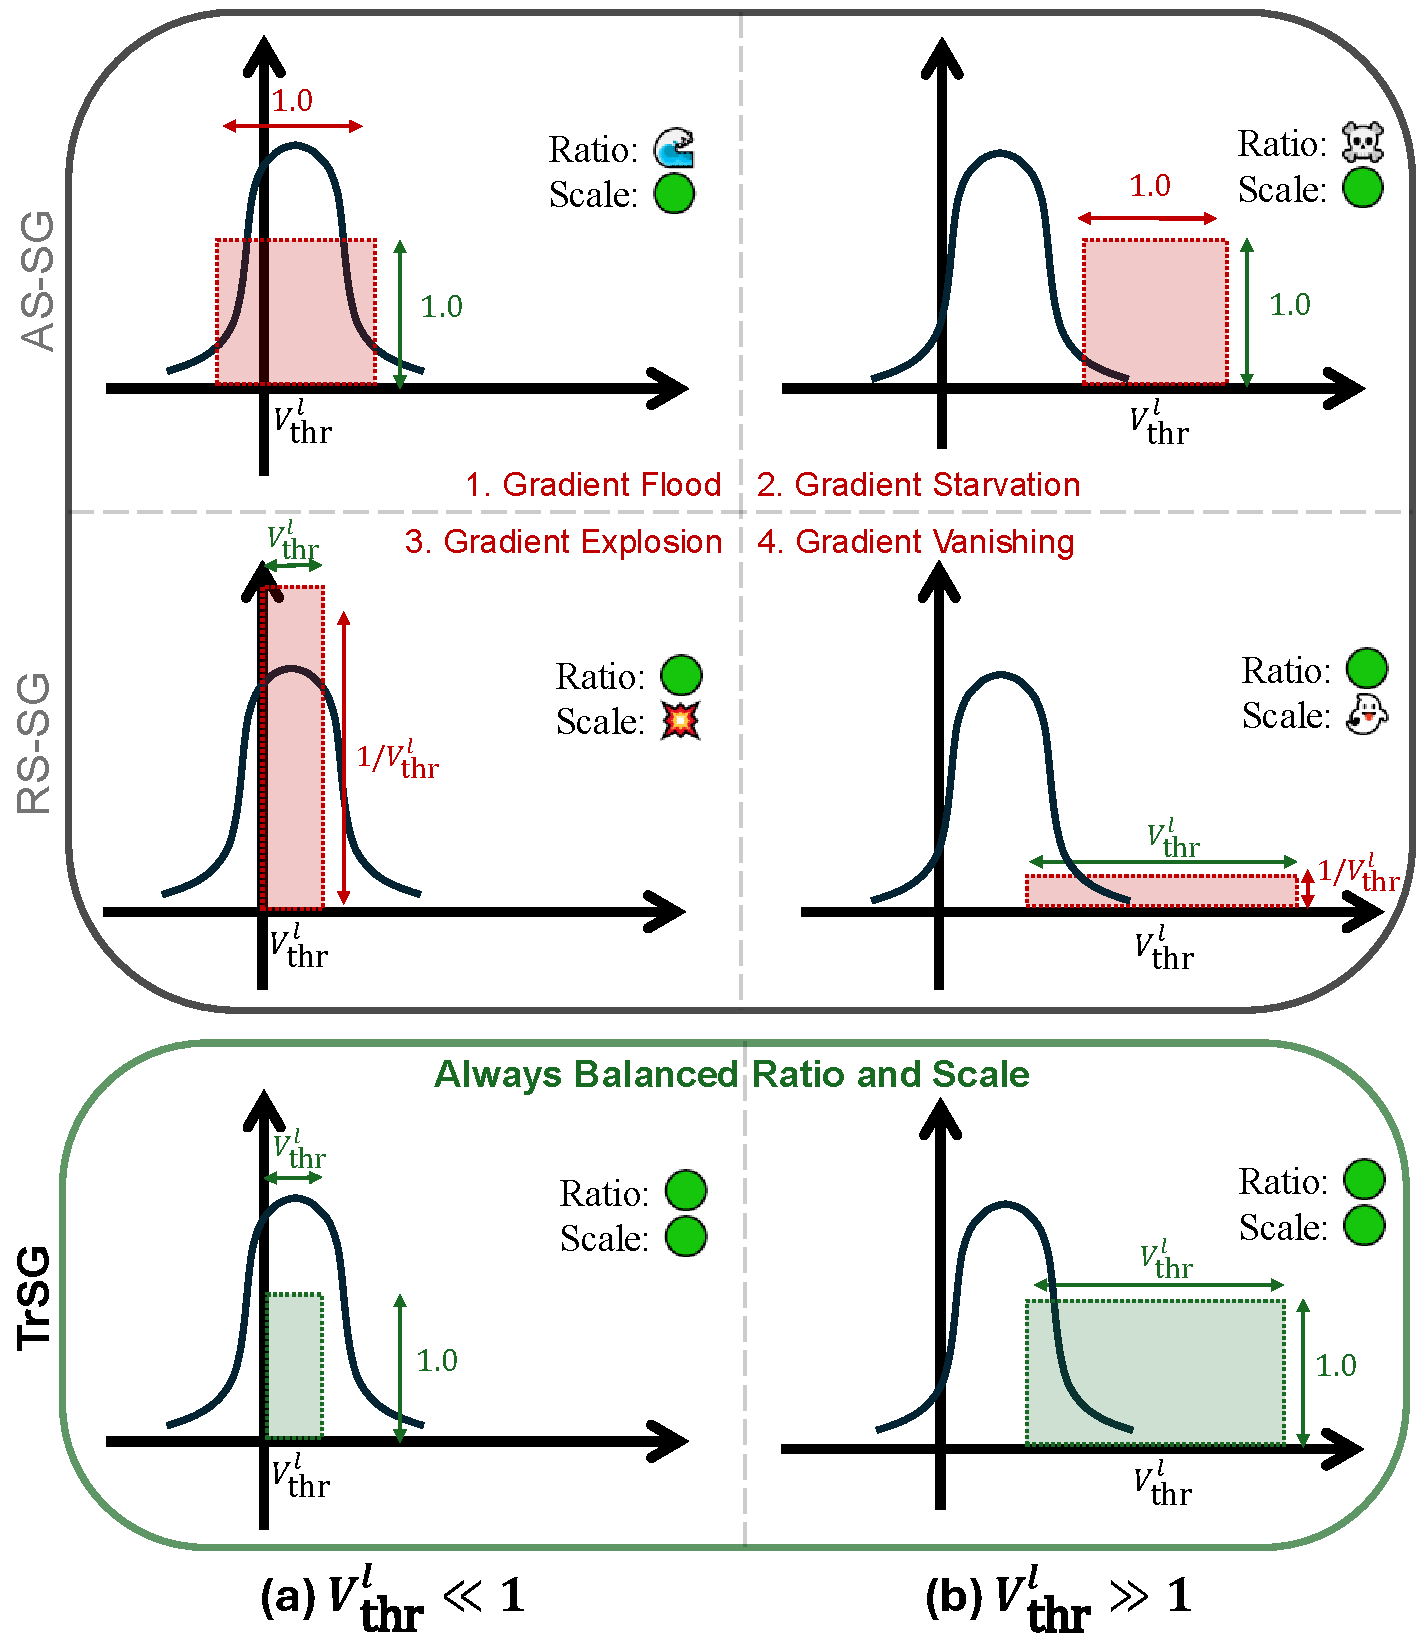
\includegraphics[width=0.99\linewidth]{fig/second_main.pdf}
    \caption{\textbf{AS-SG vs.\ RS-SG vs.\ TrSG with a rectangular surrogate gradient ($\gamma=1$).}
    The curve depicts the membrane-potential distribution; colored boxes represent the surrogate-gradient region (horizontal extent: active gradient window; vertical extent: gradient magnitude).
    Panels (a) and (b) compare small ($V_{\text{thr}}^{l}\!\ll\!1$) and large ($V_{\text{thr}}^{l}\!\gg\!1$) thresholds.
    \emph{AS-SG} uses a fixed window of width $\gamma$, leading to \textit{gradient flooding} or \textit{starvation}.
    \emph{RS-SG} normalizes the window by $V_{\text{thr}}^{l}$ but scales the magnitude as $1/V_{\text{thr}}^{l}$, causing \textit{explosion} or \textit{vanishing}.
    \textbf{TrSG} multiplies the threshold on the forward path during training, canceling the $1/V_{\text{thr}}^{l}$ factor and keeping both window and magnitude balanced.}
    \label{fig:second_main}
\end{figure}

\section{Motivation}
\label{sec:trsg_motivation}

Surrogate-gradient (SG) descent~\cite{wu:2018} enables gradient-based optimization of SNNs by replacing the non-differentiable spiking function with a differentiable surrogate near the threshold. This permits effective gradient descent and often improves performance at early timesteps. However, our analysis shows that SG used for internal neuronal parameters~\cite{fang:2021,wang:2022,rathi:2023}—particularly $V_{\text{thr}}$—makes training highly sensitive to the \emph{scale} of $V_{\text{thr}}$. While careful tuning can yield strong accuracy, this dependency exposes a fundamental limitation of current SG-based training.

In this chapter, we identify—\emph{to our knowledge for the first time}—that prior SG designs exhibit strong sensitivity of gradient flow to $V_{\text{thr}}$. To address it, we introduce \textbf{TrSG (Threshold-Robust SG)}, which maintains stable gradients regardless of the threshold value. TrSG is simple to implement, adds negligible overhead, and is compatible with a wide range of surrogate functions.

\section{Background: Surrogate Gradient Descent}
\label{sec:trsg_background}

By \cref{eq:lif_discrete_firing}, an LIF neuron emits a spike when the membrane potential crosses the threshold. Let $H(x)$ denote the Heaviside step. The spike can be written as
\[
S^{l}[t] \;=\; H\!\bigl(x(M^{l}[t],V^{l}_{\text{thr}})\bigr),
\]
where the \emph{argument} $x(\cdot)$ encodes how the membrane potential $M^{l}[t]$ and the threshold $V^{l}_{\text{thr}}$ are combined (e.g., $x = M^{l}[t]-V^{l}_{\text{thr}}$). Because $H(\cdot)$ is non-differentiable and $H'(\cdot)$ is a Dirac delta, SG training replaces $H$ with a smooth surrogate $f$ whose derivative locally approximates $H'$:
\[
H'(x)\;\approx\; f'(x)\quad\text{near }x=0.
\]
Applying the chain rule yields the working gradient
\begin{equation}
\label{eq:def_of_srgd}
\frac{\partial S^{l}[t]}{\partial M^{l}[t]}
\;=\;
H'\!\bigl(x\bigr)\,\frac{\partial x}{\partial M^{l}[t]}
\;\approx\;
f'\!\bigl(x\bigr)\,\frac{\partial x}{\partial M^{l}[t]}.
\end{equation}
The \emph{choice} of $x(\cdot)$ is crucial—especially when $V^{l}_{\text{thr}}$ is learnable—because it determines both the active region of nonzero gradients and the scaling of their magnitudes.

Reviewing the literature, SG-based methods fall into two families based on how they define $x(M^{l}[t],V^{l}_{\text{thr}})$: \emph{Absolute-Scale} (AS-SG) and \emph{Relative-Scale} (RS-SG). The distinction becomes significant once the threshold is trained.

\section{Two Families of Surrogate Gradients}
\label{sec:trsg_two_families}

To make the scaling effects explicit, we analyze a representative surrogate with a rectangular derivative
\[
f'(x) \;=\; \frac{1}{\gamma}\,\mathds{1}\!\Bigl(|x|<\tfrac{\gamma}{2}\Bigr),
\]
where $\gamma>0$ controls the width of the region where gradients flow. The phenomena described below are \emph{not} specific to this choice; any surrogate exhibits the same issues. \Cref{fig:second_main} visualizes the membrane-potential distribution under two different threshold scales: small ($V_{\text{thr}}^{l}\!\ll\!1$) and large ($V_{\text{thr}}^{l}\!\gg\!1$).

\subsection{AS-SG: Absolute-Scale Surrogate Gradient}
\label{subsec:trsg_assg}

Many works~\cite{zheng:2021, deng:2022, fang:2021, wang:2022} take
\begin{equation}
\label{eq:abs_diff_x}
x \;=\; M^{l}[t] - V^{l}_{\text{thr}},
\end{equation}
which gives
\begin{equation}
\label{eq:abs_diff_grad}
f'\!\bigl(M^{l}[t]-V^{l}_{\text{thr}}\bigr)
\;=\;
\frac{1}{\gamma}\,\mathds{1}\!\Bigl(\bigl|M^{l}[t]-V^{l}_{\text{thr}}\bigr|<\tfrac{\gamma}{2}\Bigr),
\end{equation}
and thus
\begin{equation}
\label{eq:abs_diff_sgrad}
\frac{\partial S^{l}[t]}{\partial M^{l}[t]}
\;\approx\;
f'\!\bigl(M^{l}[t]-V^{l}_{\text{thr}}\bigr).
\end{equation}
Here the active window $\{M^{l}[t]\in(V^{l}_{\text{thr}}-\tfrac{\gamma}{2},\,V^{l}_{\text{thr}}+\tfrac{\gamma}{2})\}$ has a \emph{fixed} width $\gamma$, with magnitude independent of $V^{l}_{\text{thr}}$. When $V^{l}_{\text{thr}}$ is small, the window is excessively wide relative to the membrane-potential spread, so gradients keep flowing far from the true firing boundary—a regime we term \emph{gradient flooding}. Conversely, when $V^{l}_{\text{thr}}$ is large, the fixed-width window covers only a tiny fraction of the distribution, and most gradients vanish—\emph{gradient starvation}.

\subsection{RS-SG: Relative-Scale Surrogate Gradient}
\label{subsec:trsg_rssg}

Other works normalize by the threshold, either by setting $\gamma = V^{l}_{\text{thr}}$~\cite{meng:2023} or by defining
\(
x \;=\; \tfrac{M^{l}[t]}{V^{l}_{\text{thr}}} - 1
\)
as in~\cite{rathi:2023}. In this case,
\begin{equation}
\label{eq:rel_diff_grad}
f'\!\Bigl(\tfrac{M^{l}[t]}{V^{l}_{\text{thr}}}-1\Bigr)
\;=\;
\frac{1}{\gamma}\,\mathds{1}\!\Bigl(\Bigl|\tfrac{M^{l}[t]}{V^{l}_{\text{thr}}}-1\Bigr|<\tfrac{\gamma}{2}\Bigr),
\end{equation}
so the active window $\{M^{l}[t]\in((1-\tfrac{\gamma}{2})V^{l}_{\text{thr}},\,(1+\tfrac{\gamma}{2})V^{l}_{\text{thr}})\}$ scales with $V^{l}_{\text{thr}}$. However, the chain rule introduces a sensitivity of the gradient magnitude to the threshold:
\begin{equation}
\label{eq:rel_diff_sgrad}
\frac{\partial S^{l}[t]}{\partial M^{l}[t]}
\;\approx\;
\frac{1}{V^{l}_{\text{thr}}}\,
f'\!\Bigl(\tfrac{M^{l}[t]}{V^{l}_{\text{thr}}}-1\Bigr).
\end{equation}
Thus, small thresholds amplify gradients excessively (\emph{gradient explosion}), whereas large thresholds suppress them severely (\emph{gradient vanishing}).

\section{Threshold-Robust Surrogate Gradient}
\label{sec:trsg_method}

We propose \textbf{TrSG}, a simple modification that preserves the desirable \emph{relative} window while canceling the problematic $1/V^{l}_{\text{thr}}$ factor in the gradient. During training we (i) keep the relative-scale argument,
\[
x \;=\; \frac{M^{l}[t]}{V^{l}_{\text{thr}}} - 1,
\]
and (ii) multiply the spike by the threshold on the forward path:
\begin{equation}
\label{eq:ta_srgd_core}
O^{l}[t] \;=\; V^{l}_{\text{thr}}\cdot S^{l}[t].
\end{equation}
Then,
\begin{equation}
\label{eq:ta_srgd_chainrule}
\frac{\partial O^{l}[t]}{\partial M^{l}[t]}
\;=\;
V^{l}_{\text{thr}}\;\frac{\partial S^{l}[t]}{\partial M^{l}[t]}
\;\approx\;
V^{l}_{\text{thr}}\cdot
\Bigl(\frac{1}{V^{l}_{\text{thr}}} f'(x)\Bigr)
\;=\;
f'(x),
\end{equation}
so the gradient magnitude becomes \emph{threshold-invariant} while the active window still adapts with $V^{l}_{\text{thr}}$.

\subsection{Inference Remains Binary}
\label{subsec:trsg_inference}

The threshold scaling in \cref{eq:ta_srgd_core} is training-only. At test time we revert to $S^{l}[t]\in\{0,1\}$ and absorb $V^{l}_{\text{thr}}$ into the next layer through a simple weight rescaling
\(
W^{l+1}_{l}\leftarrow V^{l}_{\text{thr}}\,W^{l+1}_{l}.
\)
Inference therefore uses standard binary spikes and a standard LIF neuron, preserving compatibility with existing neuromorphic hardware.

\paragraph{Summary.}
TrSG unifies a relative-scale argument with threshold multiplication on the forward path, ensuring stable gradients across thresholds. This design eliminates both the flooding/starvation issue of AS-SG and the vanishing/explosion problem of RS-SG.

\section{Detailed Gradient Analysis}
\label{sec:trsg_grad_analysis}

In \cref{sec:trsg_two_families,sec:trsg_method} our analysis of threshold-related instabilities centered on $\partial S^{l}[t]/\partial M^{l}[t]$, i.e., how the spike output changes with respect to the membrane potential. However, similar issues arise when considering partial derivatives with respect to the learnable internal parameters $V^{l}_{\text{thr}}$ and $\tau^{l}$. We now derive these gradients explicitly and show that AS-SG and RS-SG fail along these pathways as well, while TrSG remains stable.

\subsection{Gradient with Respect to \texorpdfstring{$V^{l}_{\text{thr}}$}{V\_thr}}
\label{subsec:trsg_grad_vthr}

Recall from \cref{eq:lif_discrete_firing} that $S^{l}[t]=\mathcal{H}\!\bigl(M^{l}[t]-V^{l}_{\text{thr}}\bigr)$. When approximating $\mathcal{H}$ by a differentiable surrogate $f_{sr}$, existing methods define the argument $x$ in either absolute-scale or relative-scale form.

\paragraph{AS-SG.}
With $x = M^{l}[t]-V^{l}_{\text{thr}}$,
\begin{equation}
\frac{\partial S^{l}[t]}{\partial V^{l}_{\text{thr}}}
\;=\;
f_{sr}'(x)\,\Bigl(\tfrac{\partial M^{l}[t]}{\partial V^{l}_{\text{thr}}} - 1\Bigr).
\end{equation}
This update does not adapt its magnitude to $V^{l}_{\text{thr}}$. Consequently, if $|V^{l}_{\text{thr}}|$ becomes very large or very small, the gradient can vanish or dominate excessively.

\paragraph{RS-SG.}
With $x = \tfrac{M^{l}[t]}{V^{l}_{\text{thr}}}-1$, the chain rule yields
\begin{equation}
\frac{\partial S^{l}[t]}{\partial V^{l}_{\text{thr}}}
\;\approx\;
f_{sr}'\!\Bigl(\tfrac{M^{l}[t]}{V^{l}_{\text{thr}}}-1\Bigr)\,\frac{\partial}{\partial V^{l}_{\text{thr}}}\!\Bigl(\tfrac{M^{l}[t]}{V^{l}_{\text{thr}}}-1\Bigr),
\end{equation}
which introduces factors proportional to $\tfrac{1}{V^{l}_{\text{thr}}}$. Tiny $V^{l}_{\text{thr}}$ explodes the gradient; huge $V^{l}_{\text{thr}}$ vanishes it.

\paragraph{TrSG.}
TrSG circumvents both extremes by adopting the relative-scale argument and multiplying $V^{l}_{\text{thr}}$ on the forward path:
\begin{equation}
O^{l}[t] \;=\; V^{l}_{\text{thr}}\,S^{l}[t].
\end{equation}
The resulting gradient of the loss $\mathcal{L}$ with respect to the threshold combines the direct effect of the multiplication and the indirect effect via the surrogate:
\begin{equation}
\frac{\partial \mathcal{L}}{\partial V^{l}_{\text{thr}}}
\;=\;
\frac{\partial \mathcal{L}}{\partial O^{l}[t]}
\Bigl(S^{l}[t] \;+\; V^{l}_{\text{thr}}\,\tfrac{\partial S^{l}[t]}{\partial V^{l}_{\text{thr}}}\Bigr).
\end{equation}
The threshold multiplication cancels the problematic $\tfrac{1}{V^{l}_{\text{thr}}}$ factor in the chain rule, keeping the gradient with respect to $V^{l}_{\text{thr}}$ stable across the full range of threshold scales.

\subsection{Gradient with Respect to \texorpdfstring{$\tau^{l}$}{tau}}
\label{subsec:trsg_grad_tau}

The leakage constant $\tau^{l}$ enters $M^{l}[t]$ through the discrete LIF update of \cref{eq:lif_discrete_potential}:
\begin{equation}
M^{l}[t] \;=\; \Bigl(1-\tfrac{1}{\tau^{l}}\Bigr) U^{l}[t-1] + \tfrac{1}{\tau^{l}} I^{l}_{\text{in}}[t].
\end{equation}
Since $\tau^{l}$ appears only in $M^{l}[t]$, it influences $S^{l}[t]$ indirectly through the chain
\begin{equation}
\frac{\partial S^{l}[t]}{\partial \tau^{l}}
\;=\;
\frac{\partial S^{l}[t]}{\partial M^{l}[t]}
\;\times\;
\frac{\partial M^{l}[t]}{\partial \tau^{l}}.
\end{equation}
If $\partial S^{l}[t]/\partial M^{l}[t]$ is poorly scaled (as in standard AS-SG or RS-SG with extreme $V^{l}_{\text{thr}}$), the corresponding gradient with respect to $\tau^{l}$ can also explode or vanish. By stabilizing the membrane-potential pathway, TrSG simultaneously stabilizes the $\tau^{l}$ pathway, ensuring well-behaved updates of the leakage constant.

\paragraph{Summary.}
TrSG's threshold-multiplication mechanism, combined with its relative-scale argument, ensures that gradients remain appropriately scaled not only along $M^{l}[t]$ but also along the $V^{l}_{\text{thr}}$ and $\tau^{l}$ pathways. This provides a uniformly stable foundation for end-to-end training of LIF SNNs with multiple learnable internal parameters.

\section{Compatibility Across Surrogate Shapes}
\label{sec:trsg_compatibility}

The TrSG construction is independent of the specific surrogate-derivative shape $f'(\cdot)$. We highlight four common choices and confirm that the threshold-invariance property of \cref{eq:ta_srgd_chainrule} carries through.

\paragraph{Rectangular.}
$f'(x) = \tfrac{1}{\gamma}\,\mathds{1}(|x|<\tfrac{\gamma}{2})$.

\paragraph{Triangular.}
$f'(x) = \tfrac{1}{\gamma^{2}}\,\max(0,\gamma-|x|)$.

\paragraph{Arctan.}
$f'(x) = \tfrac{1}{\pi}\,\tfrac{1}{1+(\pi x)^{2}}$.

\paragraph{Sigmoid.}
$f'(x) = \alpha\,\sigma(\alpha x)\,(1-\sigma(\alpha x))$.

For all four, the chain-rule cancellation in \cref{eq:ta_srgd_chainrule} eliminates the $1/V_{\text{thr}}$ factor; \cref{ch:experiments} verifies that empirical training behavior aligns with this prediction.

\section{Summary}
\label{sec:trsg_summary}

This chapter classified existing SG methods into AS-SG and RS-SG, exposed the threshold-induced gradient pathologies of each, and introduced TrSG, which restores threshold invariance with a single forward-path modification. The technique is shape-agnostic, training-only, and inference-compatible with standard LIF neurons.

    \chapter{Experiments}
\label{ch:experiments}

We evaluate \textbf{MP-Init} and \textbf{TrSG} on both static and event-based vision benchmarks: CIFAR-10, CIFAR-100~\cite{cifar}, ImageNet~\cite{imagenet}, and DVS-CIFAR10~\cite{dvscifar10}, with a variety of backbones (ResNet-19~\cite{zheng:2021}, a 7-layer CNN~\cite{tebn:2022,tab:2024}, ResNet-34~\cite{resnet}, SEW-ResNet-34~\cite{fang:2021_2}). Following tdBN~\cite{zheng:2021}, batch normalization is applied across both temporal and batch dimensions. Baselines are trained under their original configurations, and we strictly follow their reported preprocessing pipelines for fairness. We avoid strong augmentations such as AutoAugment~\cite{autoaug} or Cutout~\cite{cutout} so that the observed gains come solely from our proposed methods. Each configuration is repeated three times and we report mean$\pm$standard deviation.

\section{Experimental Setup}
\label{sec:exp_setup}

\paragraph{Architectures.}
For CIFAR-10/100~\cite{cifar} and ImageNet~\cite{imagenet} we use ResNet-19~\cite{zheng:2021} and ResNet-34~\cite{resnet}. On DVS-CIFAR10~\cite{dvscifar10} we additionally use a 7-layer CNN (64C3-AP2-128C3-128C3-AP2-256C3-256C3-AP2-1024FC-10FC) following~\cite{tebn:2022, tab:2024}. We integrate the temporal dimension into the batch dimension to ensure proper normalization, following tdBN~\cite{zheng:2021}.

In MP-Init and TrSG, the running mean of the membrane potential $\mathbb{E}[U[T]]$, the threshold $V_{\text{thr}}$, and the time-decay constant $\tau$ are layer-wise parameters. We also experimented with channel-wise versions but observed only a small difference in performance. We initialize $\mathbb{E}[U[T]]$ to $0.0$, $V_{\text{thr}}$ to $1.0$, and $\tau$ to $2.0$, following common SNN practice~\cite{deng:2022,tebn:2022,fang:2021_2,fang:2021,meng:2023,shen:2024,zhou:2024_2,shi:2024}; we do not retune these per dataset for fair comparison. The first layer acts as the stem layer that generates spikes from the input, while the final layer does not generate spikes~\cite{deng:2022}. On CIFAR-10/100 and DVS-CIFAR10, dropout is added before each fully connected layer, consistent with TEBN/TAB~\cite{tebn:2022,tab:2024}.

\paragraph{Training configuration.}
\begin{itemize}[leftmargin=2em,itemsep=2pt]
    \item \textbf{CIFAR-10/100.} ResNet-19 with timesteps $\{2,4,6\}$ on a single RTX-3090. SGD with weight decay $5\times10^{-4}$, CosineAnnealing, initial learning rate $0.02$, batch size $64$. Standard random-crop, horizontal flip, and normalization.
    \item \textbf{DVS-CIFAR10.} 7-layer CNN and ResNet-19 with timesteps $4$ and $10$. Same optimizer/scheduler as above; images cropped to $48\times 48$ and horizontally flipped, following~\cite{tebn:2022, tab:2024}.
    \item \textbf{ImageNet.} ResNet-34 trained with $T=6$, evaluated at multiple inference timesteps without fine-tuning. SGD with weight decay $4\times10^{-5}$, CosineAnnealing starting at $0.10$, batch size $512$ across $8\times$ A100-80GB with synchronized BN. SEW-ResNet-34 follows the same procedure.
\end{itemize}

\section{Effectiveness of MP-Init}
\label{sec:exp_mpinit}

We first evaluate whether MP-Init enhances final performance. \Cref{tab:mpinit_acc_impr} reports ResNet-19 accuracies on CIFAR-100 and DVS-CIFAR10 with and without MP-Init across three baselines. We observe consistent gains, not only in tdBN—which does not account for TCS—but also in TCS-aware methods (TEBN, TAB). This confirms that prior approaches address TCS only partially, while MP-Init provides a more fundamental remedy.

\begin{table}[t]
\small
\centering
\begin{tabular}{cccc}
\toprule
\textbf{Dataset}     & \textbf{Method}    & \textbf{Timestep} & \textbf{Accuracy (\%)} \\
\toprule
\multirow{6}{*}{CIFAR-100}    & tdBN      & \multirow{2}{*}{4} & 75.55 $\pm$ 0.06 \\
                             & + MP-Init &                    & \textbf{76.09 $\pm$ 0.04}    \\
\cline{2-4}
                             & TEBN      & \multirow{2}{*}{4} & 75.96 $\pm$ 0.68    \\
                             & + MP-Init &                    & \textbf{76.45 $\pm$ 0.24}    \\
\cline{2-4}
                             & TAB       & \multirow{2}{*}{4} & 76.25 $\pm$ 0.49    \\
                             & + MP-Init &                    & \textbf{77.24 $\pm$ 0.12}    \\
\hline
\multirow{6}{*}{DVS-CIFAR10} & tdBN      & \multirow{2}{*}{10} & 76.60 $\pm$ 0.20    \\
                             & + MP-Init &                     & \textbf{77.37 $\pm$ 0.38}    \\
\cline{2-4}
                             & TEBN      & \multirow{2}{*}{10} & 75.17 $\pm$ 0.50    \\
                             & + MP-Init &                     & \textbf{76.70 $\pm$ 0.78}    \\
\cline{2-4}
                             & TAB       & \multirow{2}{*}{4} & 76.43 $\pm$ 0.25    \\
                             & + MP-Init &                     & \textbf{76.93 $\pm$ 0.38}    \\
\bottomrule
\end{tabular}
\caption{Performance gains from MP-Init using ResNet-19 on CIFAR-100 and DVS-CIFAR10.}
\label{tab:mpinit_acc_impr}
\end{table}

\subsection{Impact of TCS and Role of MP-Init}
\label{subsec:exp_pca}

To visualize the effect of TCS we project the final logits of four randomly chosen classes onto two principal components. \Cref{fig:feature_split_wo_mpinit} shows that without MP-Init, classes remain entangled in early steps and only gradually separate, reflecting TCS-induced output bias. With MP-Init (\cref{fig:feature_split_w_mpinit}), class separation emerges from the very first timestep.

\begin{figure}[t]
  \centering
  \begin{subfigure}{0.32\linewidth}\centering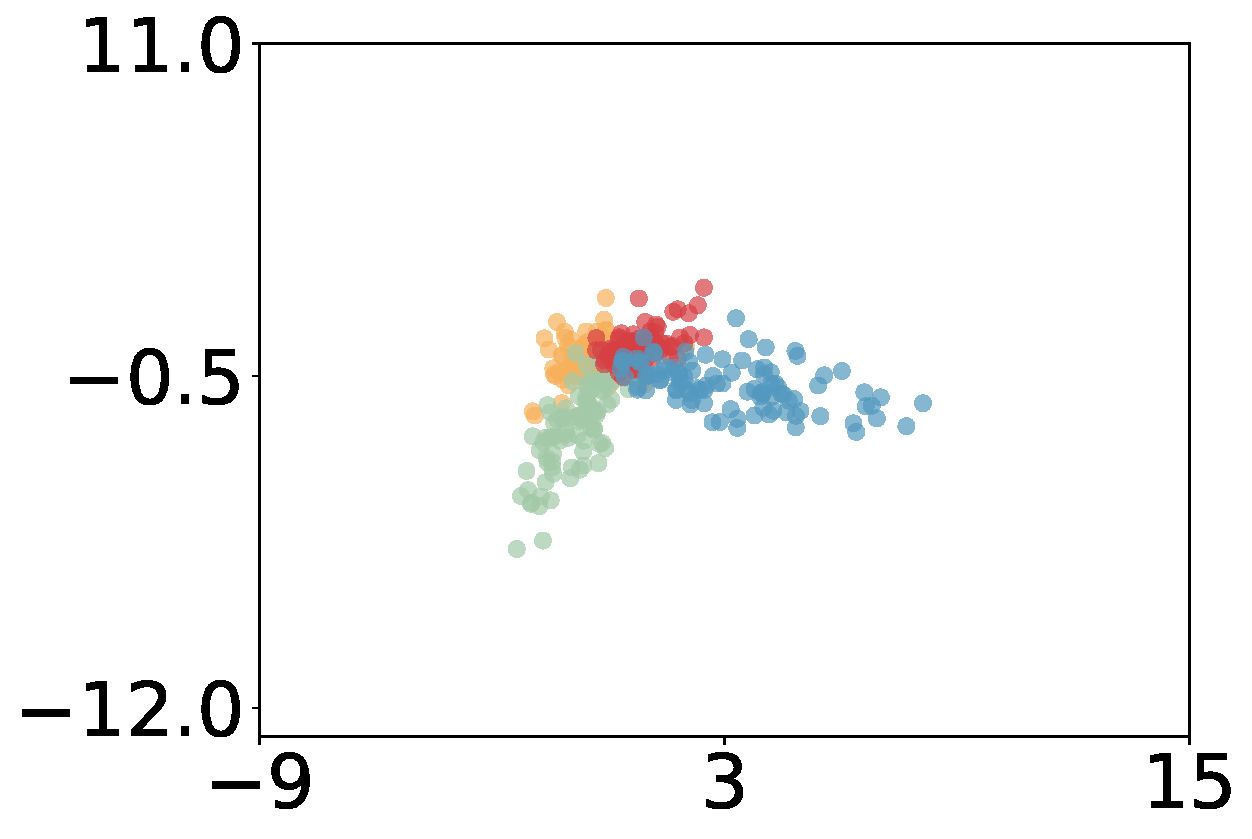
\includegraphics[width=0.995\linewidth]{fig/feature_map_not_mp_init_0.pdf}\caption{$t=1$}\end{subfigure}
  \begin{subfigure}{0.32\linewidth}\centering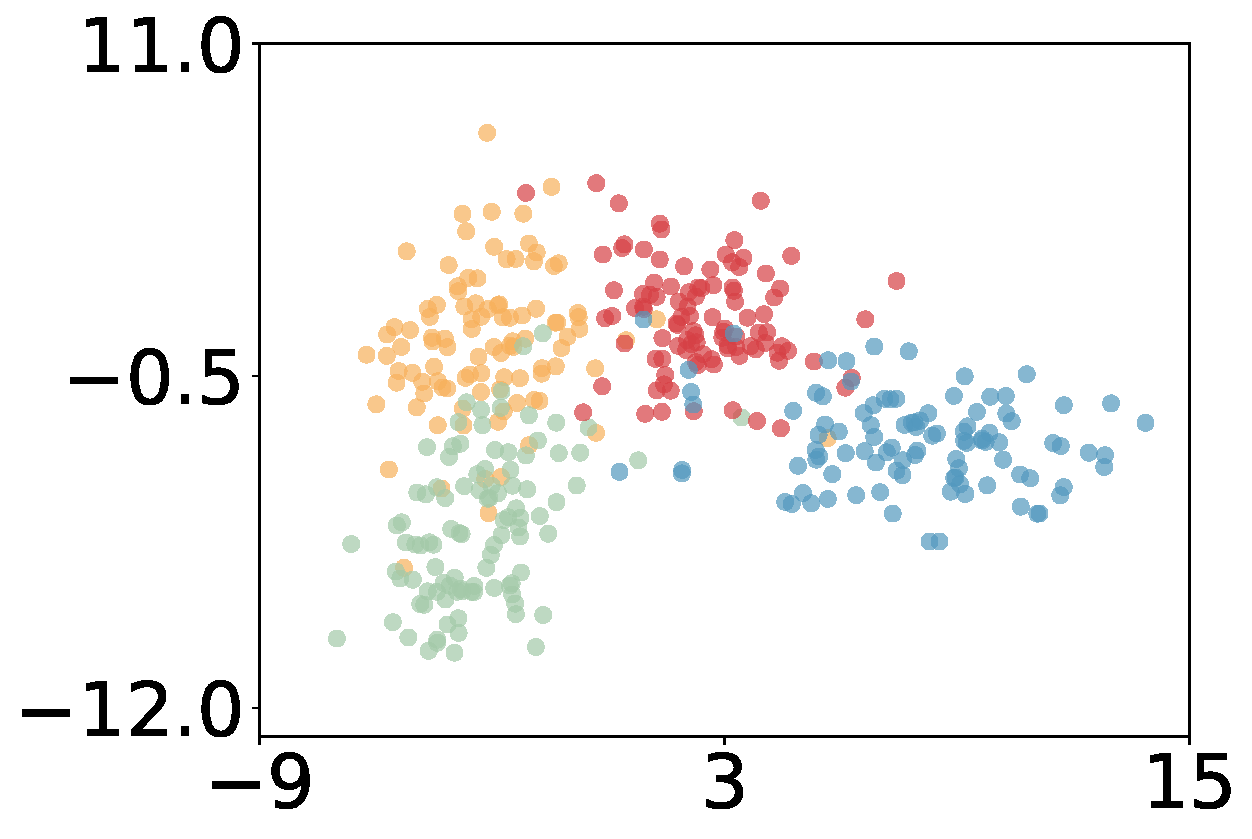
\includegraphics[width=0.995\linewidth]{fig/feature_map_not_mp_init_1.pdf}\caption{$t=2$}\end{subfigure}
  \begin{subfigure}{0.32\linewidth}\centering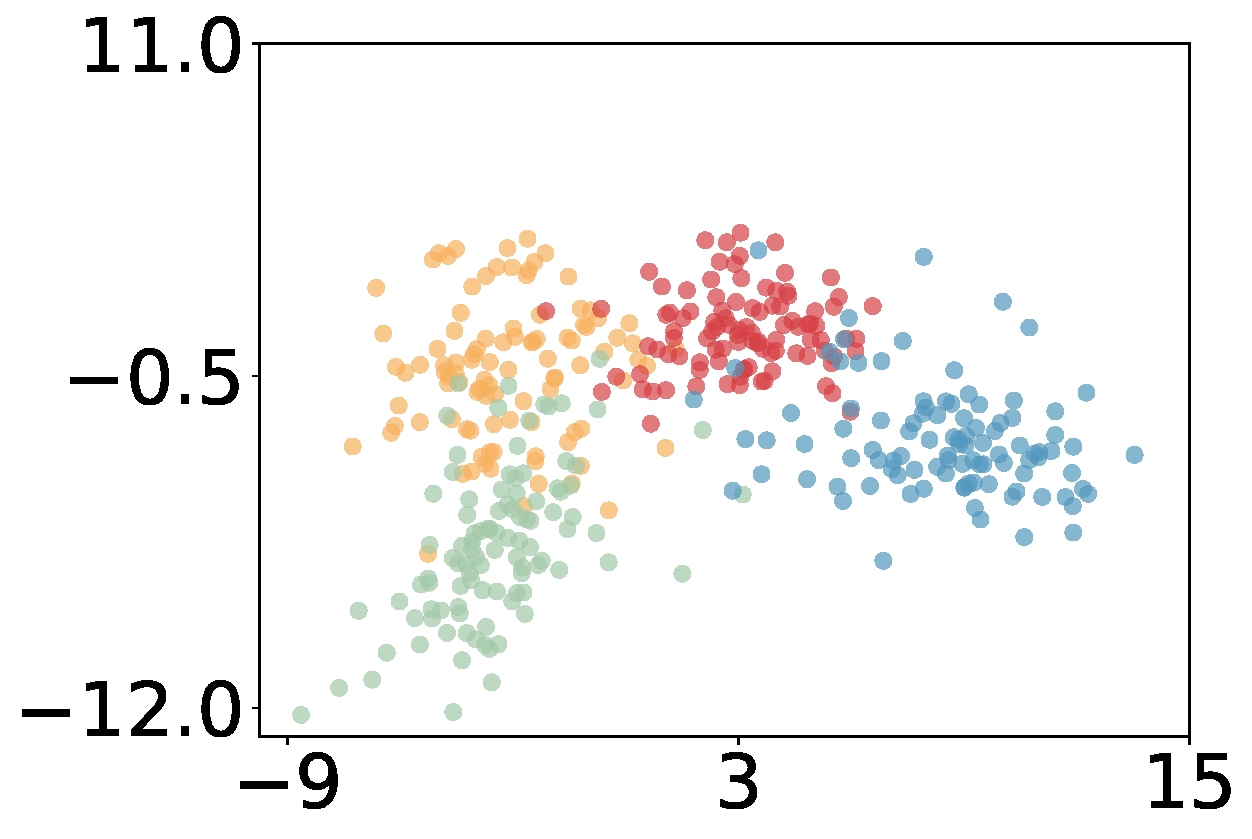
\includegraphics[width=0.995\linewidth]{fig/feature_map_not_mp_init_3.pdf}\caption{$t=4$}\end{subfigure}
  \caption{PCA of logits without MP-Init. Class clusters stay mixed in early timesteps, reflecting strong TCS.}
  \label{fig:feature_split_wo_mpinit}
\end{figure}

\begin{figure}[t]
  \centering
  \begin{subfigure}{0.32\linewidth}\centering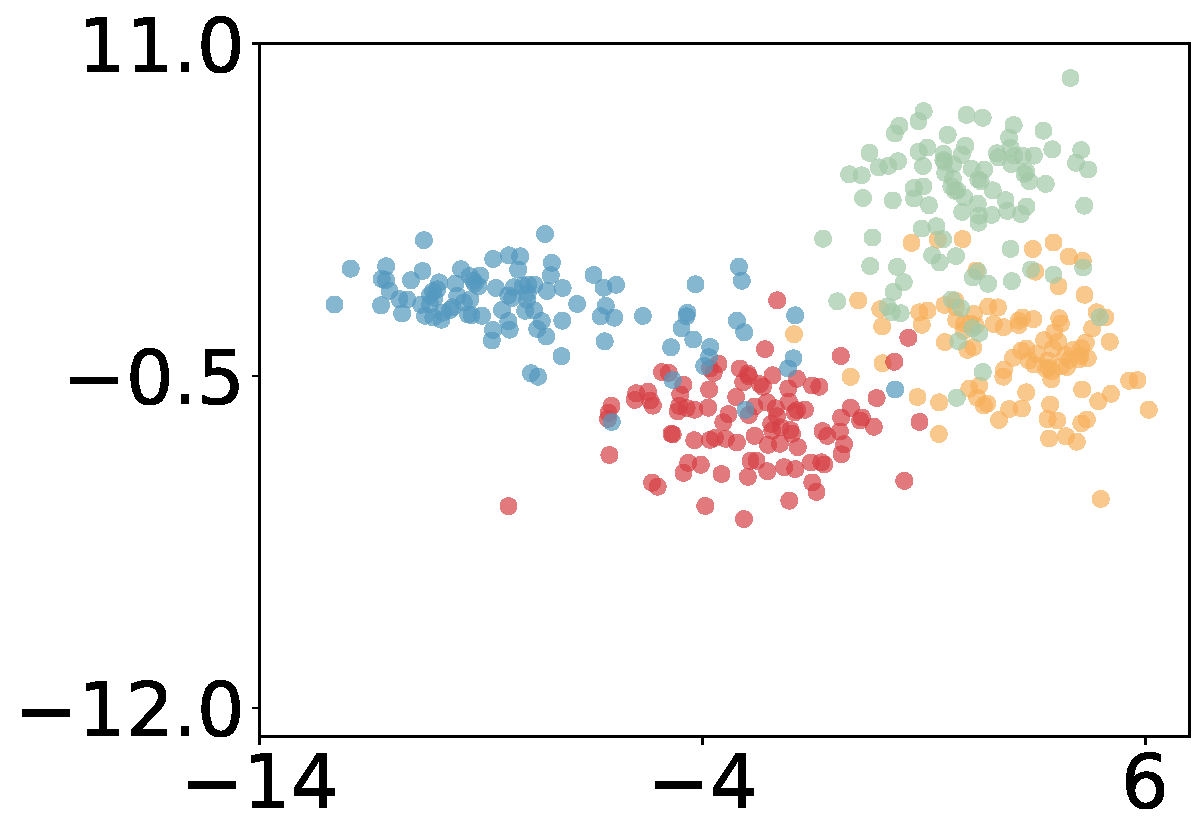
\includegraphics[width=0.995\linewidth]{fig/feature_map_mp_init_0.pdf}\caption{$t=1$}\end{subfigure}
  \begin{subfigure}{0.32\linewidth}\centering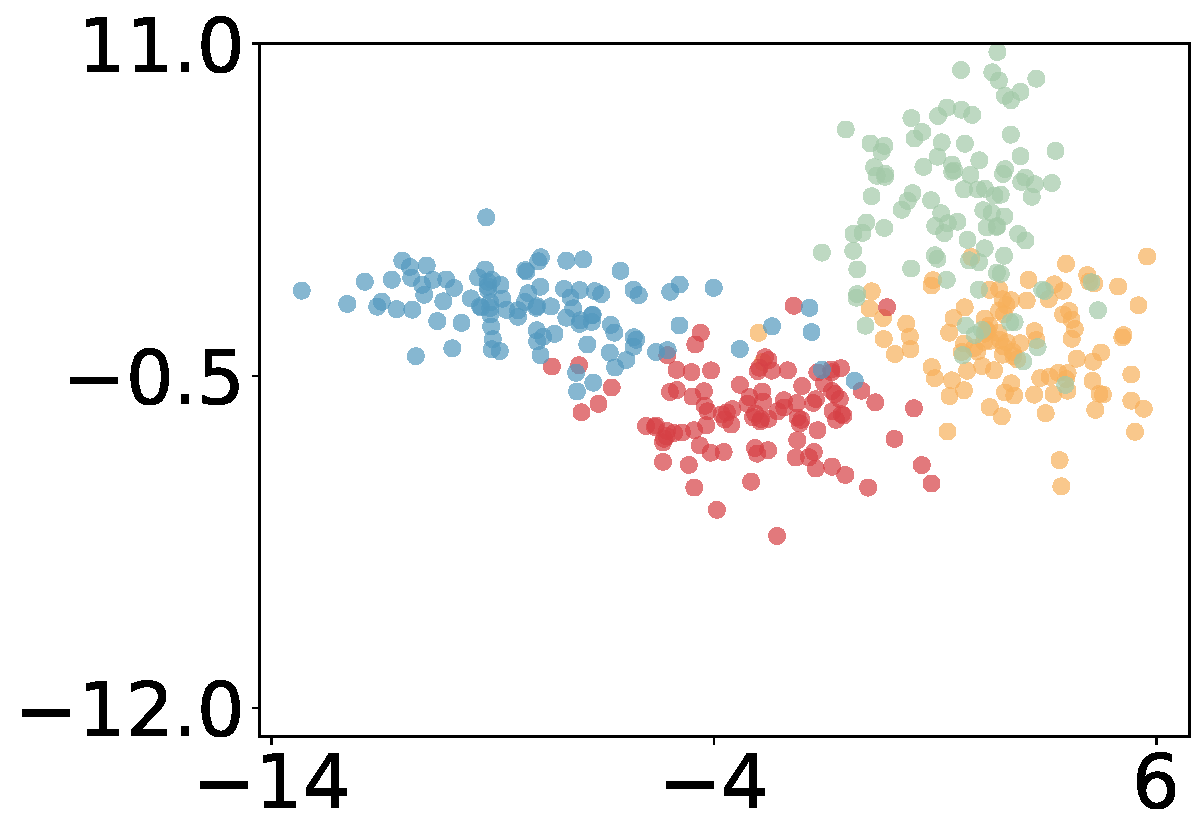
\includegraphics[width=0.995\linewidth]{fig/feature_map_mp_init_1.pdf}\caption{$t=2$}\end{subfigure}
  \begin{subfigure}{0.32\linewidth}\centering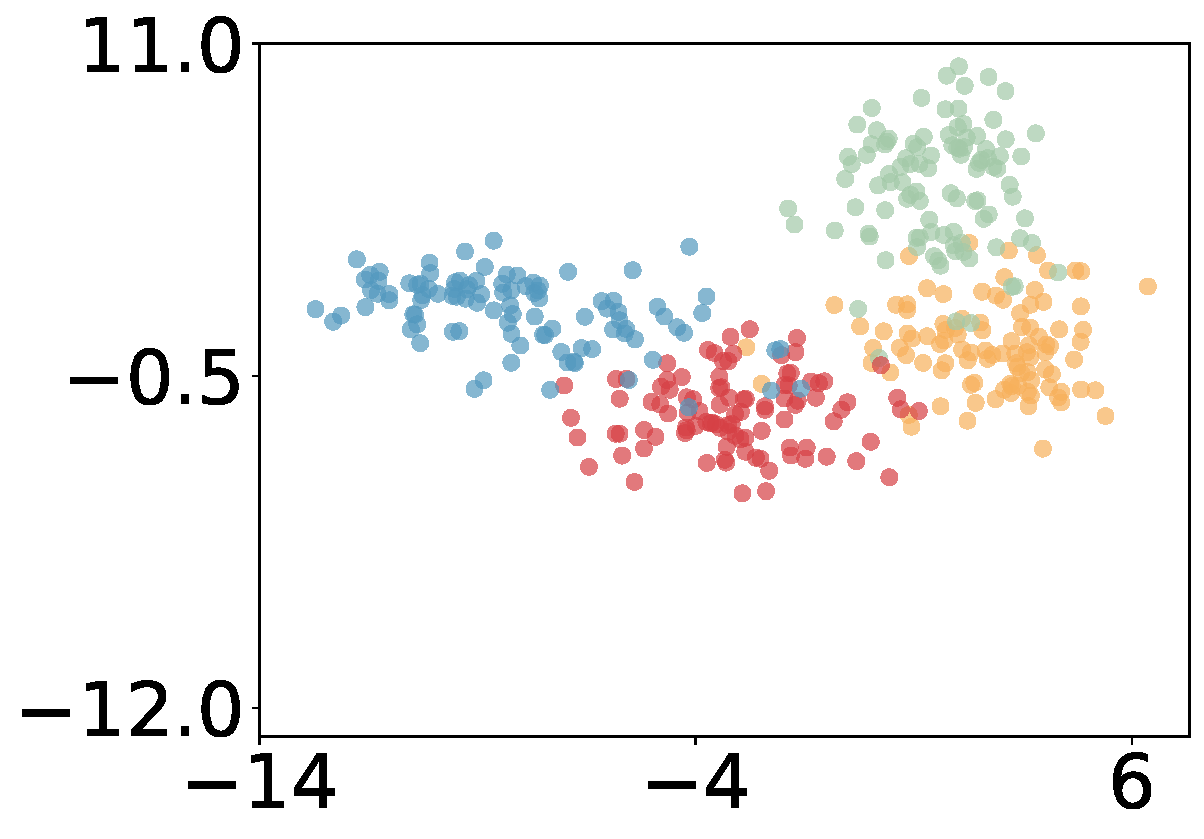
\includegraphics[width=0.995\linewidth]{fig/feature_map_mp_init_3.pdf}\caption{$t=4$}\end{subfigure}
  \caption{PCA of logits with MP-Init. Clear class separation emerges from $t=1$.}
  \label{fig:feature_split_w_mpinit}
\end{figure}

This is consistent with the firing-rate dynamics in \cref{fig:firing_rate_at_timestep}: MP-Init stabilizes neuron activations across timesteps, whereas the baseline accumulates activity over time. The class-prediction histograms in \cref{fig:classification} reinforce the picture: without MP-Init, early-step predictions collapse to a single dominant class; with MP-Init, the distribution is balanced from $t=1$.

\begin{figure}[t]
  \centering
  \begin{subfigure}{0.49\linewidth}\centering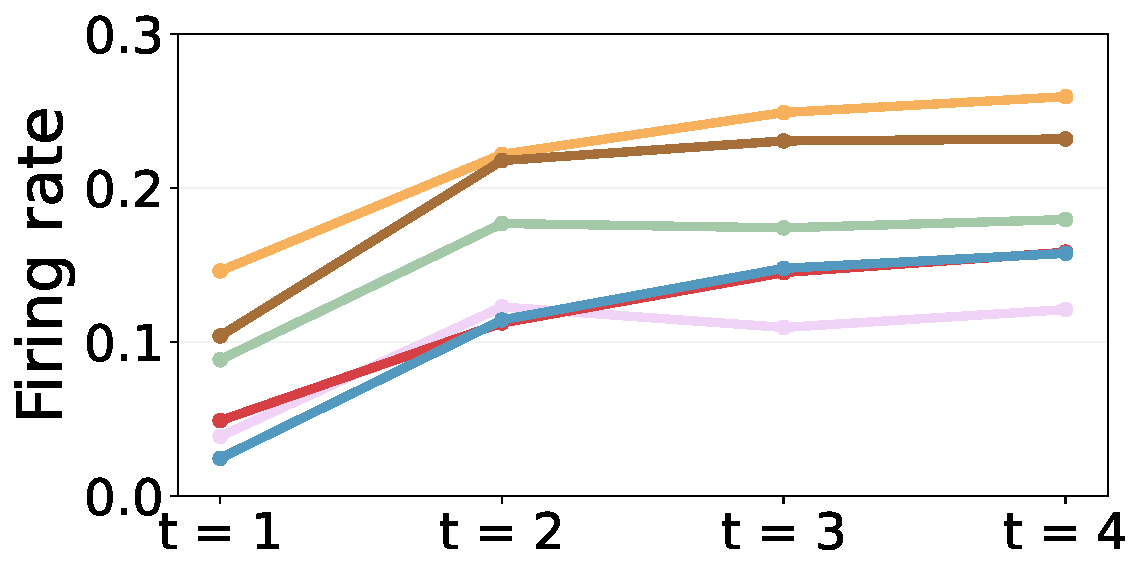
\includegraphics[width=0.99\linewidth]{fig/firing_rate_not_mp_init.pdf}\caption{w/o MP-Init}\end{subfigure}
  \hfill
  \begin{subfigure}{0.49\linewidth}\centering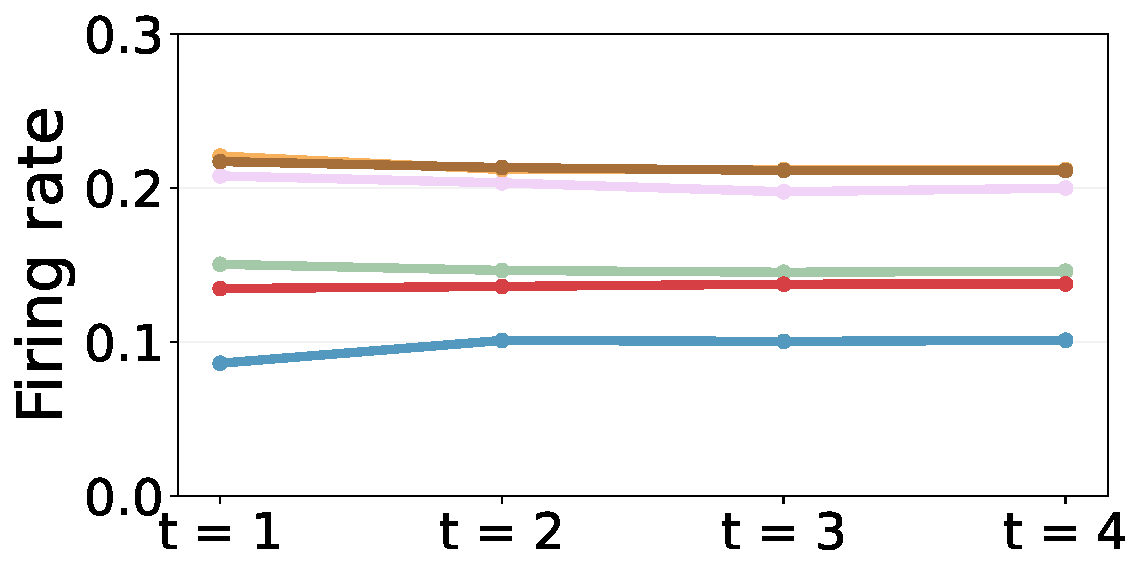
\includegraphics[width=0.99\linewidth]{fig/firing_rate_mp_init.pdf}\caption{w/ MP-Init}\end{subfigure}
  \caption{Firing rate at each timestep across six layers of ResNet-19 on CIFAR-10.}
  \label{fig:firing_rate_at_timestep}
\end{figure}

\begin{figure}[t!]
  \centering
  \begin{subfigure}{0.49\linewidth}\centering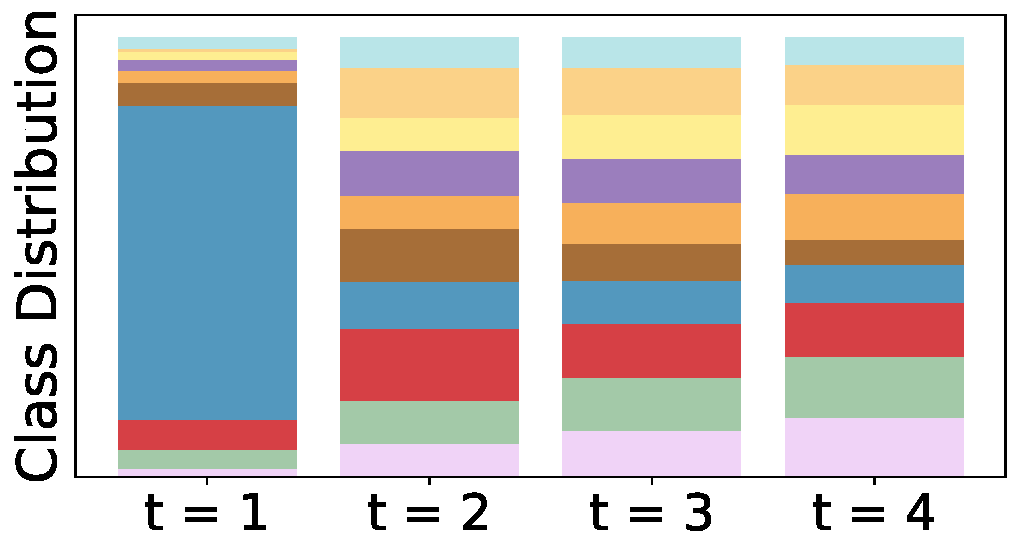
\includegraphics[width=0.99\linewidth]{fig/not_mp_init_output_rate.pdf}\caption{w/o MP-Init}\end{subfigure}
  \hfill
  \begin{subfigure}{0.49\linewidth}\centering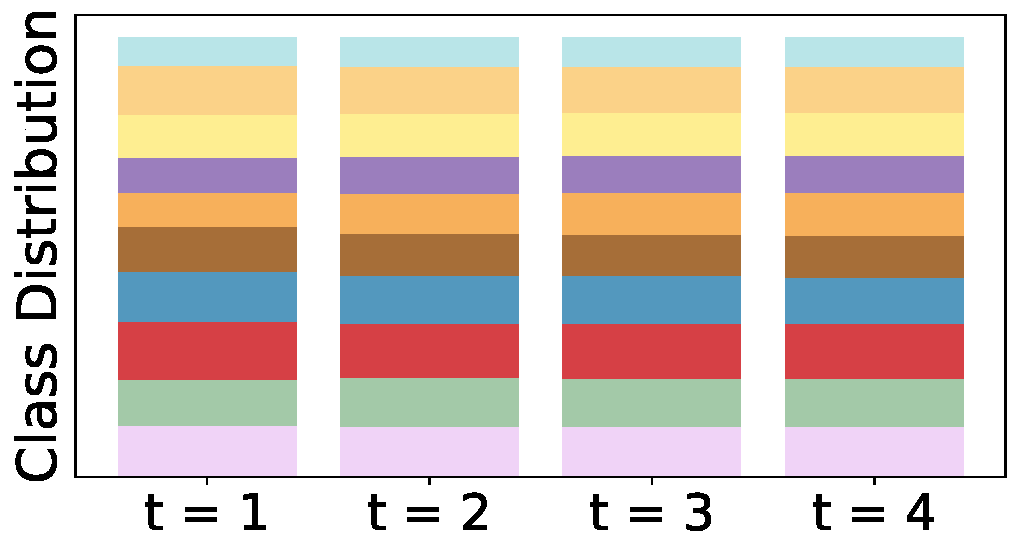
\includegraphics[width=0.99\linewidth]{fig/mp_init_output_rate.pdf}\caption{w/ MP-Init}\end{subfigure}
  \caption{Class-prediction distributions over timesteps for ResNet-19 on CIFAR-10.}
  \label{fig:classification}
\end{figure}

\subsection{Firing Rate vs.\ Accuracy}
\label{subsec:exp_pareto}

A natural concern is whether MP-Init merely increases firing and thereby harms efficiency. To test this we apply the spike-sparsity regularizer of~\cite{yan:2022} for ResNet-19 on CIFAR-100 and evaluate performance across firing rates (\cref{fig:firing_rate_vs_accuracy_mpinit}). MP-Init does not rely on excessive spiking: it forms a Pareto frontier above the baseline, achieving higher accuracy at matched or lower firing rates. Even at a firing rate of $0.06$, MP-Init outperforms all baseline settings—indicating that MP-Init enables more energy-efficient SNN operation in addition to higher accuracy.

\begin{figure}[t]
  \centering
  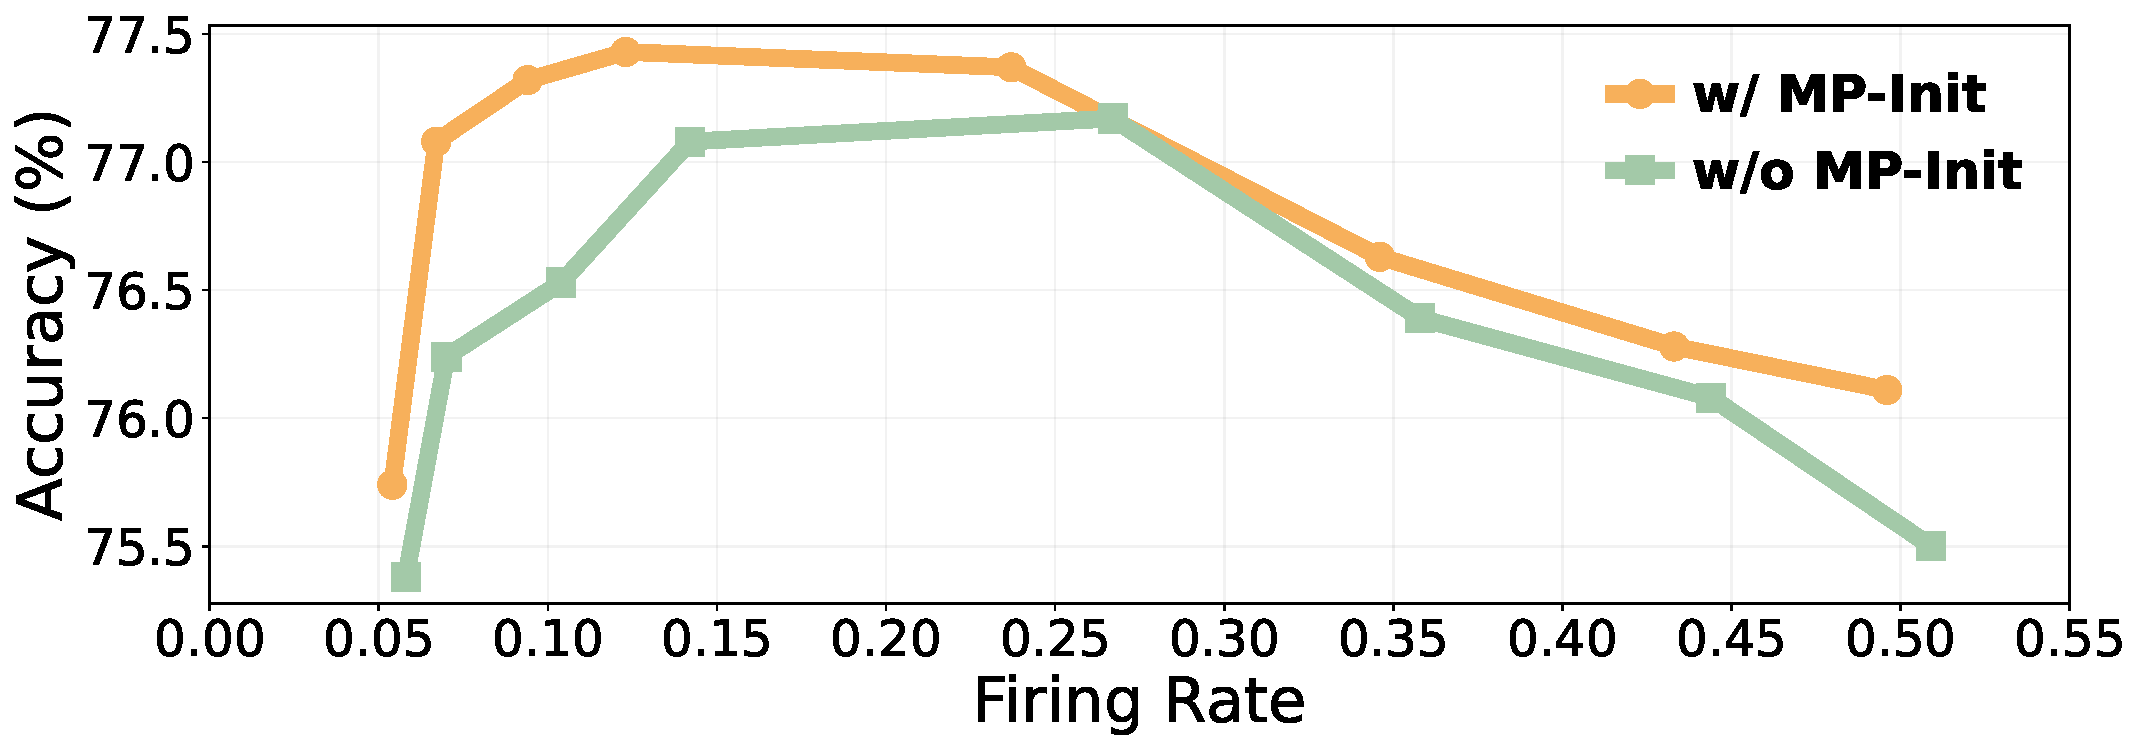
\includegraphics[width=0.7\linewidth]{fig/firing_rate_vs_accuracy.pdf}
  \caption{Accuracy vs.\ firing rate. MP-Init forms a strict Pareto frontier.}
  \label{fig:firing_rate_vs_accuracy_mpinit}
\end{figure}

\section{Effectiveness of TrSG}
\label{sec:exp_trsg}

We compare three SG approaches—\textbf{AS-SG}, \textbf{RS-SG}, and \textbf{TrSG}—when training both $V_{\text{thr}}$ and $\tau$. To ensure fair evaluation, we use the same training recipes across all methods. To assess initialization sensitivity, we sweep the initial values of $V_{\text{thr}}$ and $\tau$.

We evaluate each configuration using both \textit{soft} and \textit{hard} reset LIF neurons and two widely adopted surrogate-derivative shapes:
\begin{itemize}[leftmargin=2em,itemsep=2pt]
    \item \textbf{Rectangular}~\cite{zheng:2021,rathi:2023,wang:2022}: $f'_{sr}(x)=\tfrac{1}{\gamma}\,\mathds{1}\bigl(|x|<\tfrac{\gamma}{2}\bigr)$
    \item \textbf{Triangular}~\cite{meng:2023,deng:2022,tab:2024}: $f'_{sr}(x)=\tfrac{1}{\gamma^{2}}\max(0,\gamma-|x|)$
\end{itemize}

\Cref{fig:unified_fig}(a)--(b) (top row) shows final accuracies on CIFAR-100 with ResNet-19 across various initial $V_{\text{thr}}$. Across all conditions, \textbf{TrSG} consistently outperforms AS-SG and RS-SG, exhibiting robustness to the initial threshold. The bottom row of \cref{fig:unified_fig} shows training-loss and validation-accuracy curves: for both reset regimes, TrSG converges faster and reaches higher final accuracy. A similar trend holds when varying initial $\tau$ and when using different surrogate shapes (Arctan, Sigmoid).

\begin{figure}[t]
    \centering
    \begin{subfigure}[b]{0.48\textwidth}\centering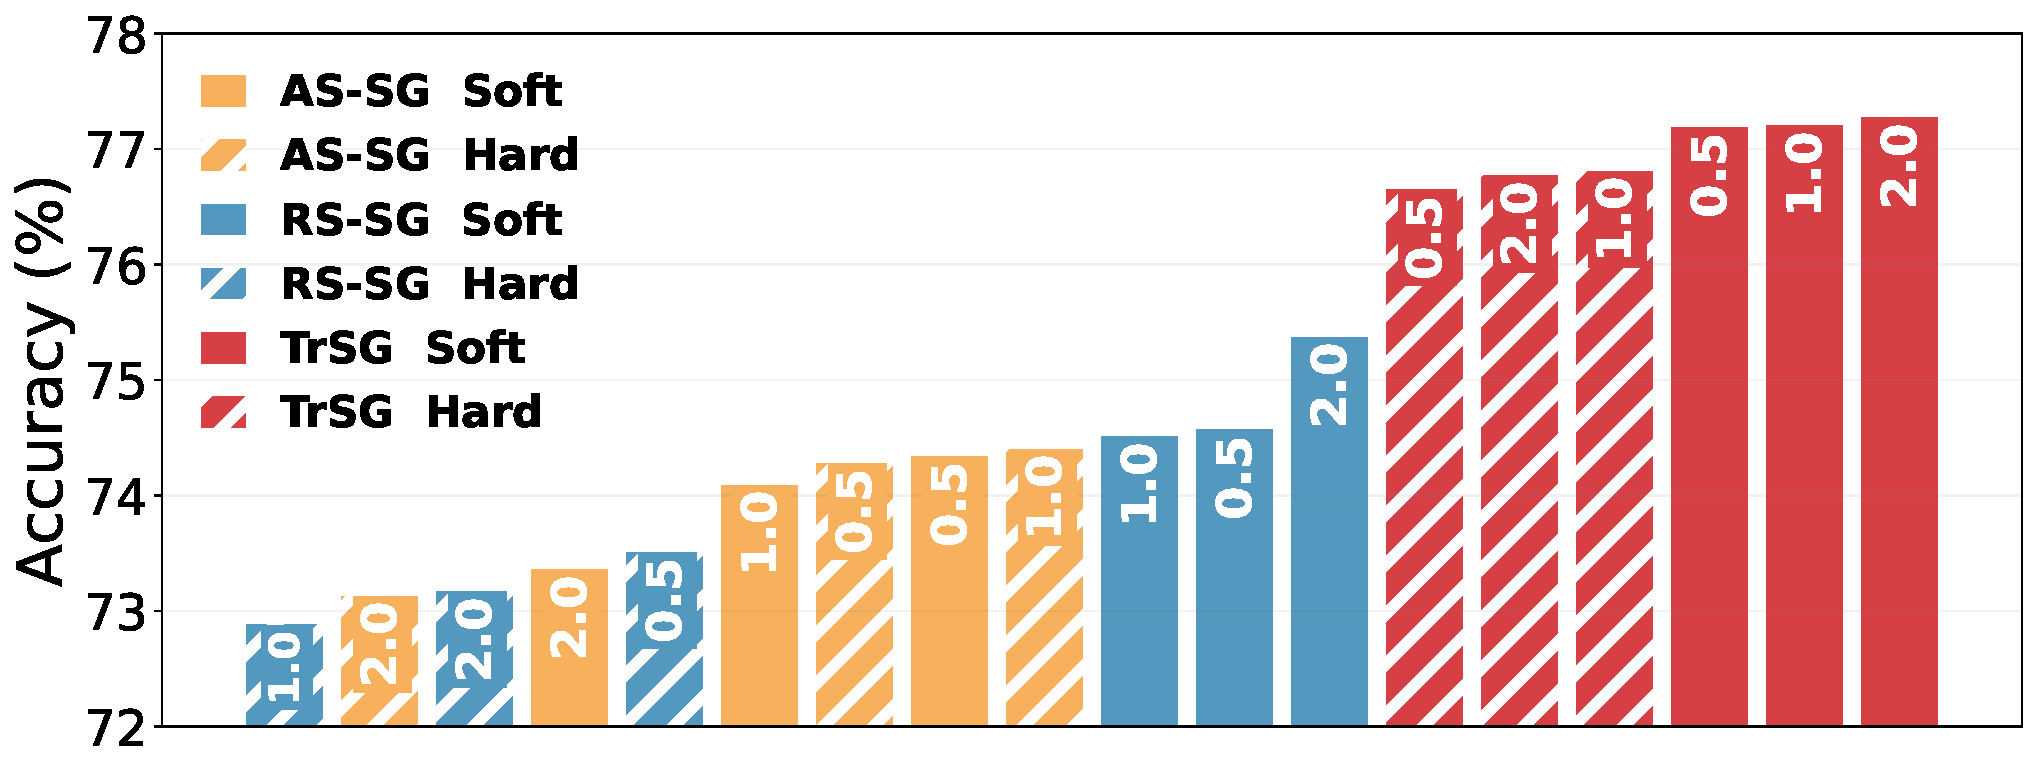
\includegraphics[width=\linewidth]{fig/acc_different_thr_rect.pdf}\caption{Rectangular}\label{fig:acc_rect}\end{subfigure}
    \hfill
    \begin{subfigure}[b]{0.48\textwidth}\centering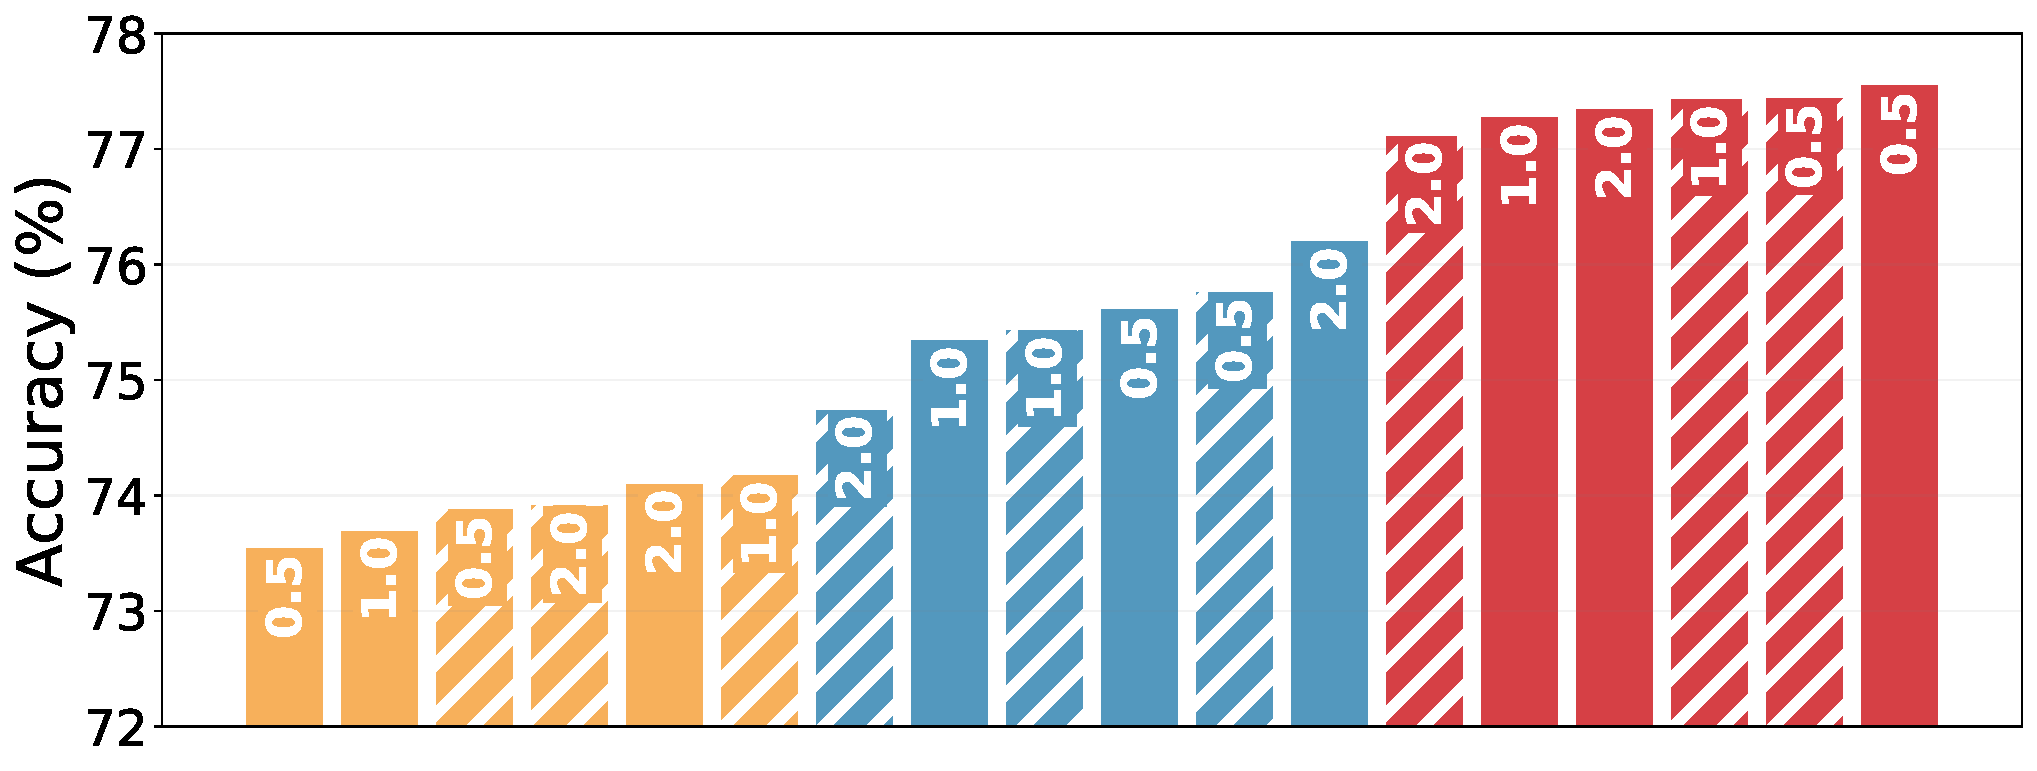
\includegraphics[width=\linewidth]{fig/acc_different_thr_tri.pdf}\caption{Triangular}\label{fig:acc_tri}\end{subfigure}
    \par\medskip
    \begin{subfigure}[b]{0.24\textwidth}\centering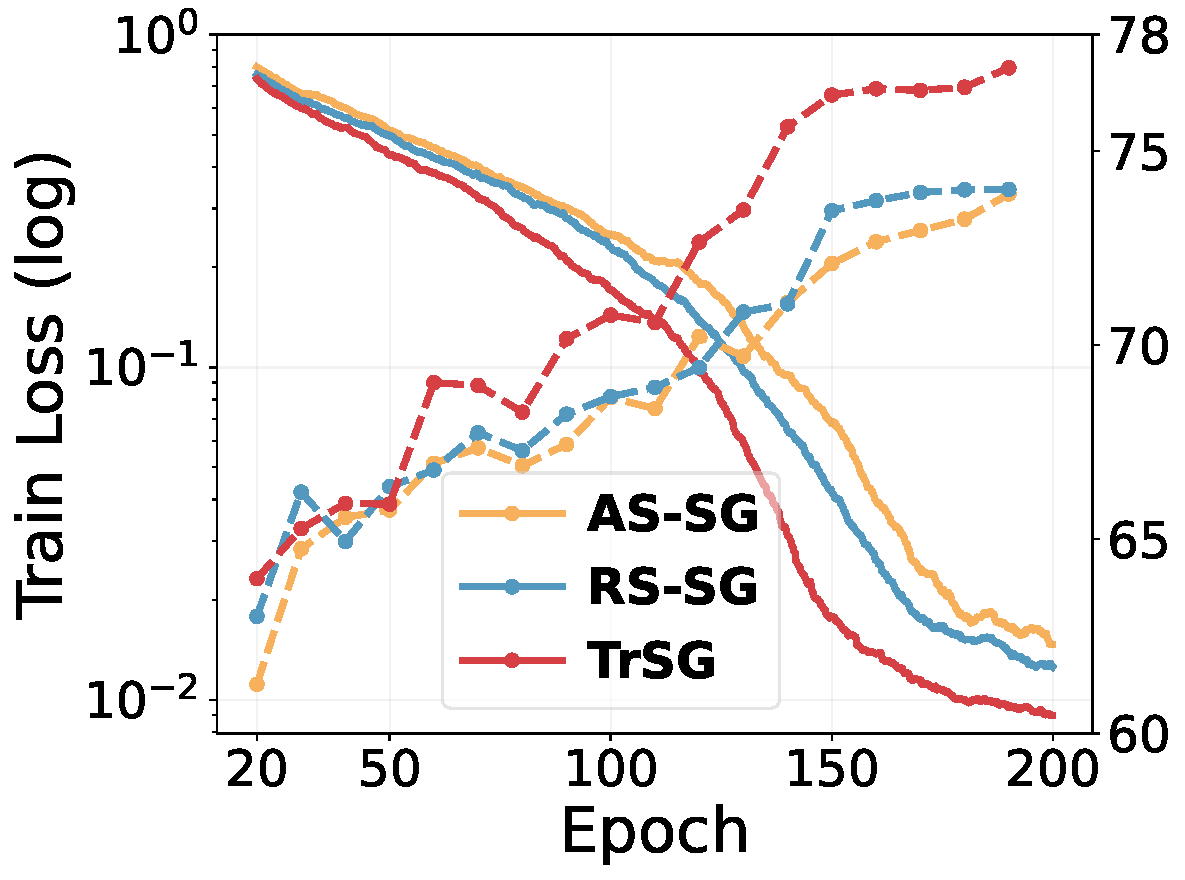
\includegraphics[width=\linewidth]{fig/loss_acc_rect_soft.pdf}\caption{Rect (soft)}\end{subfigure}
    \begin{subfigure}[b]{0.24\textwidth}\centering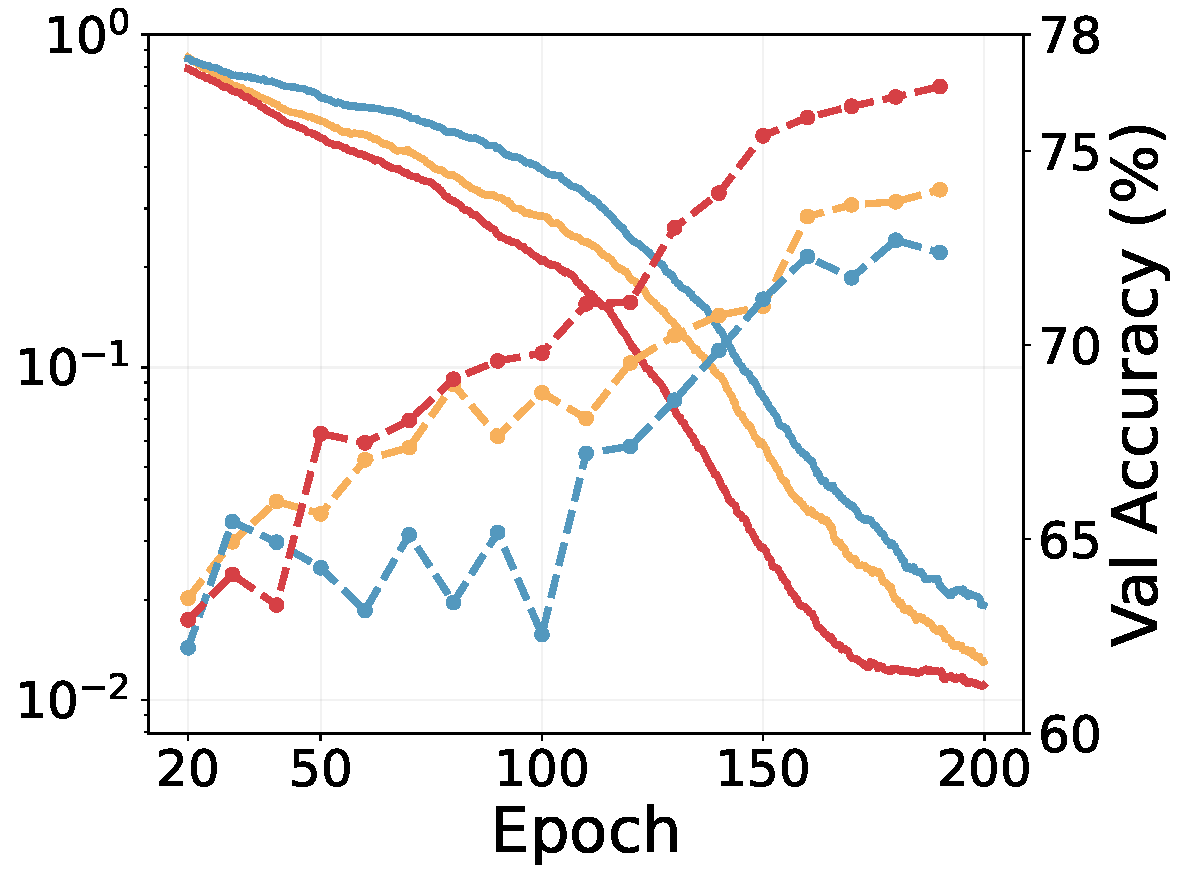
\includegraphics[width=\linewidth]{fig/loss_acc_rect_hard.pdf}\caption{Rect (hard)}\end{subfigure}
    \begin{subfigure}[b]{0.24\textwidth}\centering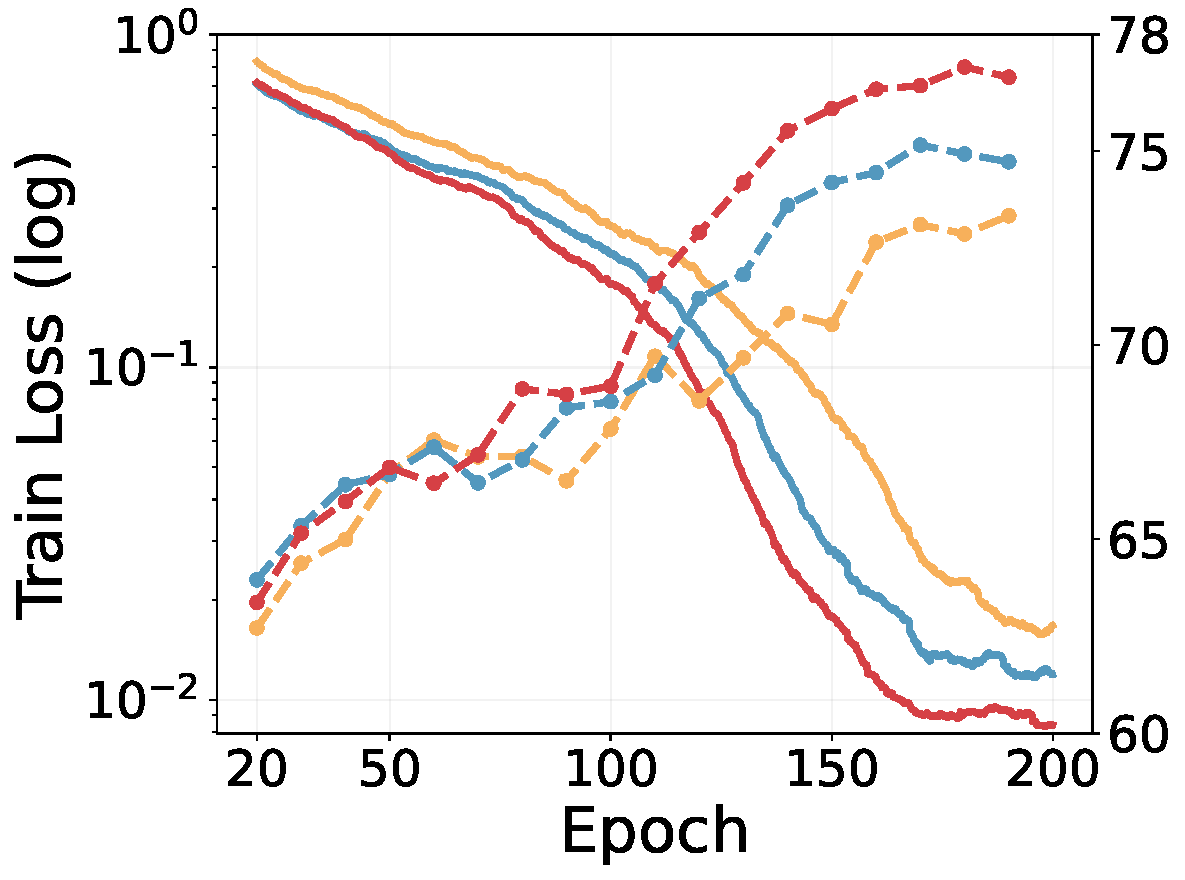
\includegraphics[width=\linewidth]{fig/loss_acc_tri_soft.pdf}\caption{Tri (soft)}\end{subfigure}
    \begin{subfigure}[b]{0.24\textwidth}\centering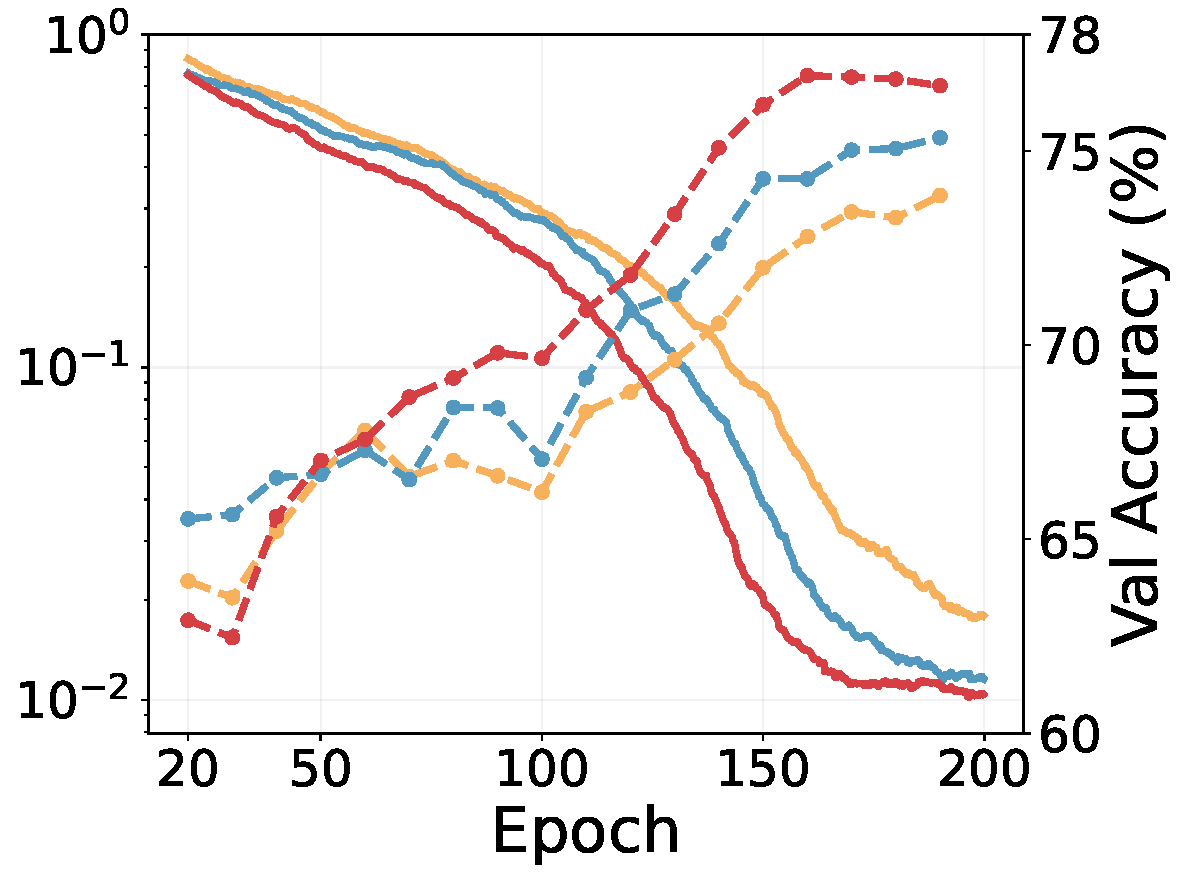
\includegraphics[width=\linewidth]{fig/loss_acc_tri_hard.pdf}\caption{Tri (hard)}\end{subfigure}
    \caption{\textbf{SG approaches under different surrogate shapes (rectangular vs.\ triangular) and reset types (soft vs.\ hard).}
    \emph{Top row:} final CIFAR-100 accuracy (ResNet-19, $T=4$) for initial $V_{\text{thr}}\in\{0.5,1.0,2.0\}$ and $\tau=2.0$.
    \emph{Bottom row:} training loss / validation accuracy curves with $\tau=2.0$, $V_{\text{thr}}=1.0$.
    TrSG consistently outperforms AS-SG and RS-SG, demonstrating robustness to initial values.}
    \label{fig:unified_fig}
\end{figure}

\section{Ablation Study}
\label{sec:exp_ablation}

\Cref{tab:ablation_table} ablates MP-Init and TrSG on ResNet-19. Both methods independently improve over the baseline; their combination yields the best result, confirming complementary contributions.

\begin{table}[h]
\small
\centering
\begin{tabular}{cccc}
\toprule
\textbf{Dataset} & \textbf{MP-Init} & \textbf{TrSG} & \textbf{Accuracy (\%)} \\
\toprule
\multirowcell{4}[0pt][c]{CIFAR-100\\(T=4)}
 & \ding{55} & \ding{55} & 75.55 $\pm$ 0.06 \\
 & \ding{51} & \ding{55} & 76.09 $\pm$ 0.04 \\
 & \ding{55} & \ding{51} & 77.15 $\pm$ 0.06 \\
 & \ding{51} & \ding{51} & \textbf{77.66 $\pm$ 0.15} \\
\midrule
\multirowcell{4}[0pt][c]{DVS-CIFAR10\\(T=10)}
 & \ding{55} & \ding{55} & 76.60 $\pm$ 0.20 \\
 & \ding{51} & \ding{55} & 77.37 $\pm$ 0.20 \\
 & \ding{55} & \ding{51} & 80.83 $\pm$ 0.64 \\
 & \ding{51} & \ding{51} & \textbf{81.43 $\pm$ 0.40} \\
\bottomrule
\end{tabular}
\caption{Ablation of MP-Init and TrSG on ResNet-19.}
\label{tab:ablation_table}
\end{table}

Building on these findings—and given their superior quality and stability—we adopt the \textbf{rectangular} surrogate function and \textbf{soft reset} as the default configuration in subsequent comparisons.

\section{Comparison with State-of-the-Art}
\label{sec:exp_sota}

We compare \textbf{MP-Init + TrSG} (referred to as ``Ours'') against state-of-the-art methods on static datasets (CIFAR-10/100, ImageNet) and the dynamic dataset DVS-CIFAR10, using standard LIF neurons and various backbones. \Cref{tab:comprehensive_results} summarizes the results.

\begin{table}[t!]
\centering
\small
\begin{tabular}{ccccc}
\toprule
\textbf{Dataset} & \textbf{Method} & \textbf{Network} & \textbf{Timestep} & \textbf{Accuracy (\%)} \\
\toprule
\multirow{5}{*}{CIFAR-10} & tdBN~\cite{zheng:2021} & \multirow{5}{*}{ResNet-19} & 2 / 4 / 6 & 92.34 / 92.92 / 93.16 \\
& TET~\cite{deng:2022} & & 2 / 4 / 6 & 94.16 / 94.44 / 94.50 \\
& TEBN~\cite{tebn:2022} & & 2 / 4 / 6 & 94.57 / 94.70 / 94.71 \\
& TAB~\cite{tab:2024} & & 2 / 4 / 6 & 94.73 / 94.76 / 94.81 \\
& \textbf{Ours} & & 2 / 4 / 6 & \textbf{95.05 $\pm$ 0.15 / 95.34 $\pm$ 0.06 / 95.50 $\pm$ 0.16} \\
\midrule
\multirow{4}{*}{CIFAR-100} & TET~\cite{deng:2022} & \multirow{4}{*}{ResNet-19} & 2 / 4 / 6 & 72.87 / 74.47 / 74.72 \\
& TEBN~\cite{tebn:2022} & & 2 / 4 / 6 & 75.86 / 76.13 / 76.41 \\
& TAB~\cite{tab:2024} & & 2 / 4 / 6 & 76.31 / 76.81 / 76.82 \\
& \textbf{Ours} & & 2 / 4 / 6 & \textbf{76.87 $\pm$ 0.16 / 77.66 $\pm$ 0.15 / 77.91 $\pm$ 0.32} \\
\midrule
\multirow{12}{*}{ImageNet} & tdBN~\cite{zheng:2021} & \multirow{4}{*}{ResNet-34} & 6 & 63.72 \\
& Dspike~\cite{li:2021} & & 6 & 68.19 \\
& TEBN~\cite{tebn:2022} & & 4 & 64.29 \\
& TAB~\cite{tab:2024} & & 4 & 67.78 \\
\cline{2-5}
& SEW-ResNet~\cite{fang:2021_2} & \multirow{6}{*}{SEW-ResNet-34} & 4 & 67.04 \\
& TET~\cite{deng:2022} & & 4 & 68.00 \\
& TEBN~\cite{tebn:2022} & & 4 & 68.28 \\
& IMP+LTS~\cite{shen:2024} & & 4 & 68.90 \\
& MPS~\cite{ding:2025} & & 4 & 69.03 \\
& EAGD~\cite{yang:2025} & & 4 & 68.12 \\
\cline{2-5}
& \multirow{2}{*}{\textbf{Ours}} & ResNet-34 & 4 / 6 & 67.15 $\pm$ 0.03 / \textbf{68.73 $\pm$ 0.09} \\
& & SEW-ResNet-34 & 4 & \textbf{69.67 $\pm$ 0.08} \\
\midrule
\multirow{8}{*}{DVS-CIFAR10} & tdBN~\cite{zheng:2021} & \multirow{3}{*}{ResNet-19} & 10 & 67.80 \\
& MPBN~\cite{guo:2023_2} & & 10 & 74.40 $\pm$ 0.20 \\
& RMP-Loss~\cite{guo:2023} & & 10 & 76.20 $\pm$ 0.20 \\
\cline{2-5}
& BNTT~\cite{bntt:2020} & \multirow{3}{*}{7-layer CNN} & 20 & 63.20 \\
& TEBN~\cite{tebn:2022} & & 10 & 75.10 \\
& TAB~\cite{tab:2024} & & 4 & 76.70 \\
\cline{2-5}
& \multirow{2}{*}{\textbf{Ours}} & ResNet-19 & 10 & \textbf{81.43 $\pm$ 0.40} \\
&  & 7-layer CNN & 4 & \textbf{79.27 $\pm$ 0.75} \\
\bottomrule
\end{tabular}
\caption{Comprehensive comparison of our methods on static and dynamic datasets.}
\label{tab:comprehensive_results}
\end{table}

\paragraph{CIFAR-10/100.} Ours achieves the best accuracy across all evaluated timesteps. On CIFAR-10 we reach $95.50\%$ at $T=6$, improving over the previous best (TAB at $94.81\%$) by $0.69$\%pt. On CIFAR-100 we obtain $77.91\%$ at $T=6$, surpassing the strongest baseline (TAB at $76.82\%$) by $1.09$\%pt. Our results at fewer timesteps already outperform baselines at larger timesteps, highlighting improved efficiency.

\paragraph{ImageNet.} With ResNet-34, our method reaches $68.73\%$ top-1 accuracy at $T=6$. With SEW-ResNet-34 we further reach $69.67\%$ at $T=4$, outperforming IMP+LTS~\cite{shen:2024} ($68.90\%$) and MPS~\cite{ding:2025} ($69.03\%$). Unlike those approaches, ours adds negligible overhead and does not require neuron-specific extra parameters or complex optimization.

\paragraph{DVS-CIFAR10.} With ResNet-19 at $T=10$ we obtain $81.43\%$, exceeding the previous best (RMP-Loss at $76.20\%$). With a lightweight 7-layer CNN we still reach $79.27\%$ at $T=4$.

\section{Extensions to Advanced Architectures and Tasks}
\label{sec:exp_extensions}

We further evaluate MP-Init and TrSG on \textbf{Transformer-based SNNs}. On DVS-CIFAR10 (10 timesteps) our method improves SpikeFormer2 from $78.90\%$ to \textbf{$80.10\%$} and QKFormer from $83.80\%$ to \textbf{$84.80\%$}. On ImageNet (4 timesteps) SpikingResformer rises from $74.34\%$ to \textbf{$75.62\%$}, and QKFormer from $78.80\%$ to \textbf{$79.90\%$} (\cref{tab:advanced_snn}). The +$1.0$--$1.3$\%pt gains indicate that MP-Init and TrSG transfer cleanly to advanced Transformer backbones without architectural changes.

\begin{table}[h]
\centering
\small
\begin{tabular}{llc}
\toprule
\textbf{Dataset} & \textbf{Architecture} & \textbf{Accuracy (\%)} \\
\midrule
\multirow{7}{*}{DVS-CIFAR10}
& Spikformer~\cite{zhou2023spikformer} & 80.90 \\
& Spikingformer~\cite{zhou2023spikingformer} & 81.30 \\
& S-Transformer~\cite{yao2023stransformer} & 80.00 \\
& SpikeFormer2~\cite{zhou:2024} & 78.90 \\
& \quad + \textbf{Ours} & \textbf{80.10} \\
& QKFormer~\cite{zhou:2024_2} & 83.80 \\
& \quad + \textbf{Ours} & \textbf{84.80} \\
\midrule
\multirow{7}{*}{ImageNet}
& Spikformer~\cite{zhou2023spikformer} & 70.24 \\
& Spikingformer~\cite{zhou2023spikingformer} & 72.45 \\
& S-Transformer~\cite{yao2023stransformer} & 72.28 \\
& SpikingResformer~\cite{shi:2024} & 74.34 \\
& \quad + \textbf{Ours} & \textbf{75.62} \\
& QKFormer~\cite{zhou:2024_2} & 78.80 \\
& \quad + \textbf{Ours} & \textbf{79.90} \\
\bottomrule
\end{tabular}
\caption{Transformer-based SNNs with and without our method. DVS-CIFAR10 is evaluated at 10 timesteps; ImageNet at 4 timesteps. Baselines are matched in parameter budget.}
\label{tab:advanced_snn}
\end{table}

Beyond classification, we validate task generality on COCO-2017 detection with EMS-ResNet10~\cite{su:2023}. With identical training configurations (100 epochs) for the baseline and ours, MP-Init + TrSG improves mAP from $0.291$ to \textbf{$0.305$} (mAP@0.5) and from $0.138$ to \textbf{$0.147$} (mAP@0.5:0.95), as summarized in \cref{tab:object_detection}.

\begin{table}[h]
\centering
\small
\begin{tabular}{lc}
\toprule
\textbf{Architecture} & \textbf{COCO2017 (mAP@0.5 / mAP@0.5:0.95)} \\
\midrule
EMS-ResNet10~\cite{su:2023} & 0.291 / 0.138 \\
\quad + \textbf{Ours} & \textbf{0.305 / 0.147} \\
\bottomrule
\end{tabular}
\caption{Object detection on COCO-2017 with EMS-ResNet10 ($T=3$).}
\label{tab:object_detection}
\end{table}

\section{How Does MP-Init Impact Training?}
\label{sec:exp_mpinit_impact}

TEBN~\cite{tebn:2022} and TAB~\cite{tab:2024} have shown that temporal covariate shift indeed occurs, and \cref{ch:mpinit} demonstrated that MP-Init effectively resolves it. Prior studies, however, did not provide direct evidence of \emph{how} TCS impairs training. Inspired by the ensemble interpretation of SNNs in MPS~\cite{ding:2025}, we revisit this question with a gradient-conflict experiment on ResNet-19 with CIFAR-100. We compute the gradients applied to a given layer at each timestep and measure the cosine similarity across timesteps.

As shown in \cref{fig:gradient_conflict_tcs}, without MP-Init (left) the gradients at $t=1$ exhibit strong conflicts with later timesteps, indicating severe inconsistency across the temporal ensemble members. With MP-Init (right), these conflicts are largely alleviated and the overall cosine similarity improves. This provides direct evidence that TCS not only degrades inference consistency but also hinders gradient alignment during training, and confirms that MP-Init effectively stabilizes optimization.

\begin{figure}[h]
    \centering
    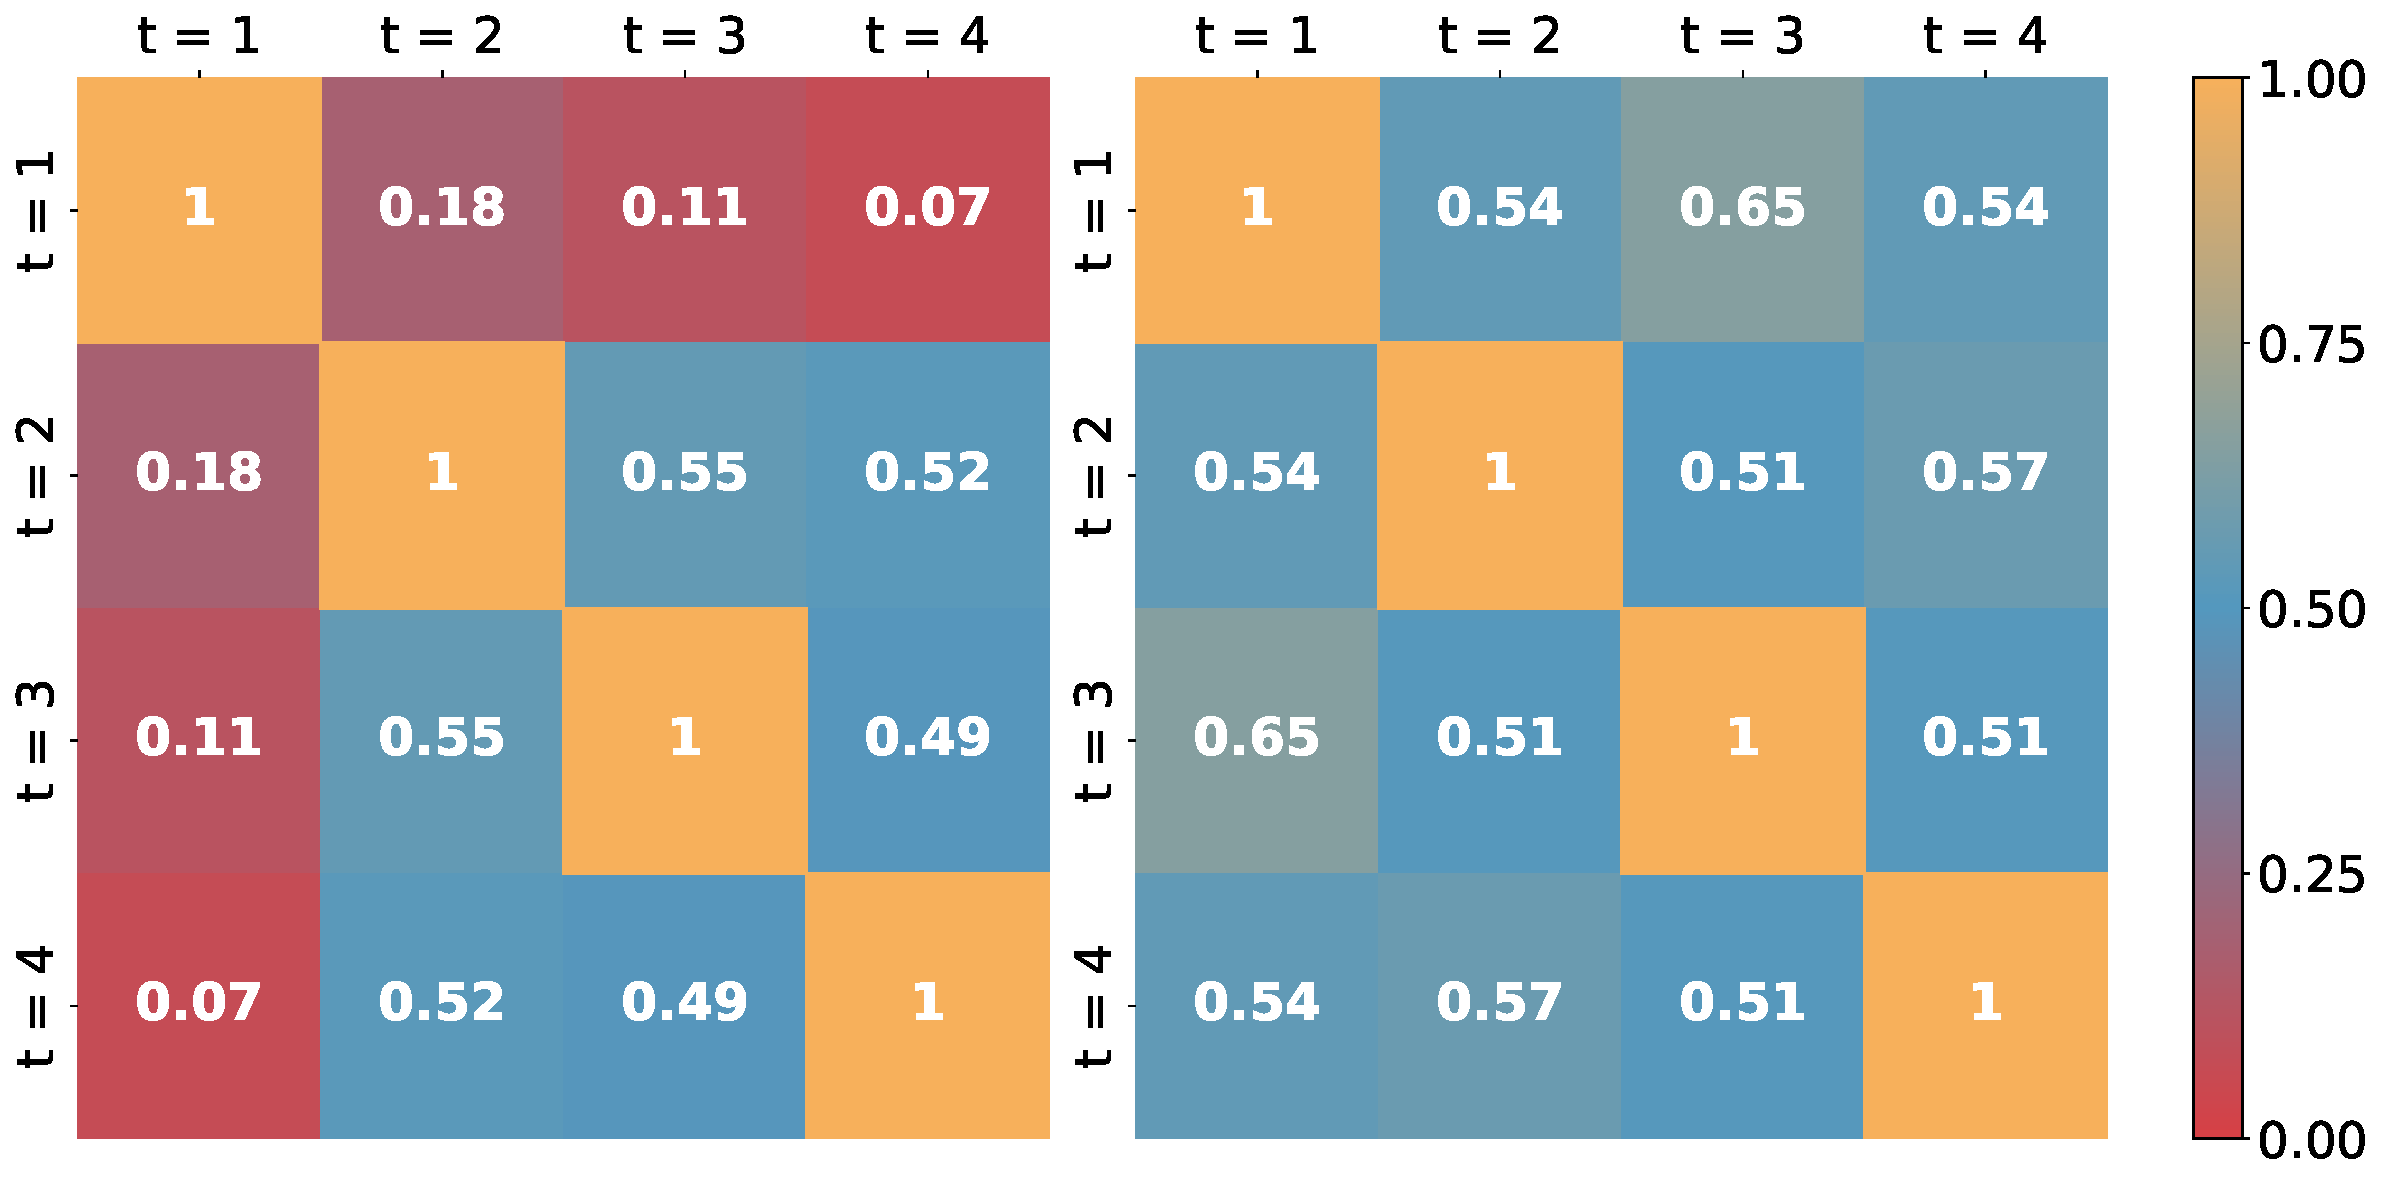
\includegraphics[width=0.99\linewidth]{fig/grad_collision.pdf}
    \caption{\textbf{Gradient conflicts across timesteps with and without MP-Init.} Cosine similarity of gradients across timesteps in ResNet-19 on CIFAR-100. \emph{Left:} Without MP-Init, the gradient from $t=1$ strongly conflicts with later timesteps, reflecting the temporal inconsistency highlighted by MPS~\cite{ding:2025}. \emph{Right:} With MP-Init, conflicts are largely resolved and similarities improve, indicating that MP-Init aligns temporal ensemble members and stabilizes training.}
    \label{fig:gradient_conflict_tcs}
\end{figure}

\section{How Does TrSG Impact Training?}
\label{sec:exp_trsg_impact}

We analyze the gradient flow of ResNet-19 on CIFAR-100 with $T=4$ for 200 epochs. To isolate the effect of the SG formulation, we \emph{fix} $\tau=2.0$ and freeze both $V_{\text{thr}}$ and $\tau$. We use a rectangular surrogate with $\gamma=1$ and a soft-reset mechanism.

\paragraph{Stability metrics.}
We quantify gradient stability with three complementary metrics computed over the convolutional weights of a given layer:
\begin{align}
\text{AbsStr} &= \operatorname*{mean}_{i} |g_{i}|, \\
\text{RatioAG} &= \frac{1}{N}\sum_{i} \mathds{1}\!\bigl(|x_{i}|<\tfrac{\gamma}{2}\bigr), \\
\text{GradCV} &= \frac{\operatorname{std}_{i}(|g_{i}|)}{\operatorname*{mean}_{i}(|g_{i}|)},
\end{align}
where $g_{i}=\partial \mathcal{L}/\partial W_{i}$ and $x_{i}$ is the surrogate argument. \textbf{AbsStr} measures average gradient magnitude—very low values indicate vanishing, very high values indicate explosion, and stable training requires moderate values. \textbf{RatioAG} is the fraction of neurons receiving nonzero gradients—too low yields gradient starvation, too high yields gradient flood, and an intermediate range is ideal. \textbf{GradCV} captures variability of gradient magnitudes—a low CV ($<1$) implies smooth, balanced updates handled by a single learning rate, whereas $\mathrm{CV}\gg1$ means some weights update disproportionately faster than others, destabilizing training. TrSG is designed to maintain moderate AbsStr, healthy RatioAG, and low GradCV simultaneously.

\subsection{Reference Case: $V_{\text{thr}}=1.0$}
\label{subsec:exp_trsg_metric_ref}

With the widely used threshold $V_{\text{thr}}=1.0$, all SG variants behave identically (\cref{tab:metrics_ref}). Although $1.0$ is not necessarily optimal, it serves as a sanity check: from epoch~1 to epoch~100 we observe steadily improving yet stable gradients across AS-SG, RS-SG, and TrSG.

\begin{table}[h]
\centering
\small
\begin{tabular}{ccccc}
\toprule
\textbf{Epoch} & $V_{\text{thr}}{=}1.0$ & \textbf{AbsStr} & \textbf{RatioAG (\%)} & \textbf{GradCV} \\
\midrule
1   & any SG & 0.0122 & 6.72  & 0.818 \\
100 & any SG & 0.0211 & 18.97 & 0.571 \\
\bottomrule
\end{tabular}
\caption{Reference case where all SG variants behave identically (ResNet-19, CIFAR-100, $T=4$, $\tau=2.0$).}
\label{tab:metrics_ref}
\end{table}

\subsection{Low Threshold Stress Test: $V_{\text{thr}}=0.1$}
\label{subsec:exp_trsg_metric_low}

This stress test exposes small-threshold failure modes (\cref{tab:metrics_low}). At epoch~1, AS-SG floods (its wide window covers a too-large fraction of the membrane distribution), RS-SG explodes due to the $1/V_{\text{thr}}$ factor (AbsStr is over $1700\times$ larger than TrSG's), while TrSG remains stable. By epoch~100, AS-SG still shows instability with $\mathrm{RatioAG}=90.20\%$ (extreme flooding), and RS-SG diverges to NaN. TrSG trains smoothly throughout. The accuracy outcomes of \cref{tab:no_training_results} below are consistent with these dynamics.

\begin{table}[h]
\centering
\small
\begin{tabular}{ccccc}
\toprule
\textbf{Epoch} & $V_{\text{thr}}{=}0.1$ & \textbf{AbsStr} & \textbf{RatioAG (\%)} & \textbf{GradCV} \\
\midrule
\multirow{3}{*}{1} & AS-SG & 0.2756 & 31.25 & 5.01  \\
                   & RS-SG & 7.8191 & 0.01  & 37.11 \\
                   & TrSG  & 0.0046 & 3.05  & \textbf{0.861} \\
\midrule
\multirow{3}{*}{100} & AS-SG & 0.0145 & 90.20 & 1.22  \\
                     & RS-SG & NaN    & 0.00  & NaN   \\
                     & TrSG  & 0.0153 & 21.45 & \textbf{0.865} \\
\bottomrule
\end{tabular}
\caption{Low-threshold stress test (CIFAR-100, $T=4$, $\tau=2.0$). RS-SG diverges, AS-SG floods, while TrSG remains stable.}
\label{tab:metrics_low}
\end{table}

\subsection{High Threshold Stress Test: $V_{\text{thr}}=2.0$}
\label{subsec:exp_trsg_metric_high}

For the large threshold $V_{\text{thr}}=2.0$, the absolute window of AS-SG is too narrow and the $1/V_{\text{thr}}$ factor in RS-SG suppresses signals (\cref{tab:metrics_high}). AS-SG starves (its activation ratio collapses to $0\%$ by epoch~100, with literally zero gradient flow), and RS-SG vanishes with high variance ($\mathrm{GradCV}=2.247$). TrSG preserves stable updates throughout.

\begin{table}[h]
\centering
\small
\begin{tabular}{ccccc}
\toprule
\textbf{Epoch} & $V_{\text{thr}}{=}2.0$ & \textbf{AbsStr} & \textbf{RatioAG (\%)} & \textbf{GradCV} \\
\midrule
\multirow{3}{*}{1} & AS-SG & 0.0058 & 0.78 & 17.14 \\
                   & RS-SG & 0.0066 & 1.64 & 0.639 \\
                   & TrSG  & 0.0092 & 1.62 & \textbf{0.961} \\
\midrule
\multirow{3}{*}{100} & AS-SG & 0.0000 & 0.00 & 0.000 \\
                     & RS-SG & 0.0021 & 0.10 & 2.247 \\
                     & TrSG  & 0.0323 & 6.90 & \textbf{0.731} \\
\bottomrule
\end{tabular}
\caption{High-threshold stress test (CIFAR-100, $T=4$, $\tau=2.0$). AS-SG starves, RS-SG vanishes, TrSG preserves stable updates.}
\label{tab:metrics_high}
\end{table}

\subsection{Accuracy with Frozen Internal Parameters}
\label{subsec:exp_no_training}

\Cref{tab:no_training_results} reports final accuracy when both $V_{\text{thr}}$ and $\tau$ are \emph{frozen} (so as to isolate the SG effect), with $\tau=2.0$ and $V_{\text{thr}}\in\{0.1,0.5,1.0,1.5,2.0\}$. Conventional SGs fail outside a narrow range—exploding at $0.1$, starving or vanishing at $2.0$—while TrSG remains robust across all thresholds.

\begin{table}[h]
\centering
\small
\begin{tabular}{cc|ccccc}
\toprule
\textbf{Reset} & \textbf{SG} & \multicolumn{5}{c}{$\boldsymbol{V_{\text{thr}}}$} \\
\cmidrule(lr){3-7}
\multicolumn{2}{c|}{} & 0.1 & 0.5 & 1.0 & 1.5 & 2.0 \\
\midrule
\multirow{3}{*}{\textbf{Soft}}
  & AS-SG          & 61.59          & 75.96          & ---            & 69.97          & 18.09 \\
  & RS-SG          & \emph{div.}    & 76.12          & ---            & 71.43          & 5.43  \\
  & \textbf{TrSG}  & \textbf{73.99} & \textbf{76.82} & \textbf{75.56} & \textbf{71.97} & \textbf{64.27} \\
\midrule
\multirow{3}{*}{\textbf{Hard}}
  & AS-SG          & 67.71          & \textbf{76.34} & ---            & 68.42          & 12.27 \\
  & RS-SG          & 10.36          & 75.85          & ---            & 72.51          & 52.10 \\
  & \textbf{TrSG}  & \textbf{68.94} & 76.33          & \textbf{75.72} & \textbf{73.86} & \textbf{68.42} \\
\bottomrule
\end{tabular}
\caption{Accuracy (\%) with fixed $\tau=2.0$ and \emph{frozen} $V_{\text{thr}}$ to isolate SG effects. TrSG remains robust across thresholds, while AS-SG and RS-SG fail outside a narrow range.}
\label{tab:no_training_results}
\end{table}

\subsection{Trajectories of Trainable Thresholds}
\label{subsec:exp_threshold_trajectories}

The discussion above raises a natural question: \emph{do real trainings actually visit such extreme thresholds?} The answer is yes. When $V_{\text{thr}}$ is trainable, many layers drift toward \emph{lower} thresholds (often $\ll 1$), while late or deep layers move \emph{upward} toward larger values (around $\sim2$ on CIFAR-100, and even higher on ImageNet). \Cref{fig:vthr_dynamics} summarizes these trajectories. CIFAR-100 and DVS-CIFAR10 show several early layers dropping below $1$ and the last layer increasing, whereas ImageNet exhibits a wider spread with some deep layers rising well beyond $2$. These observations confirm that the brittle regimes identified for AS-SG and RS-SG are encountered in practice—precisely where TrSG's threshold-robustness is most beneficial.

\begin{figure}[t!]
  \centering
  \begin{subfigure}[b]{0.32\linewidth}
    \centering
    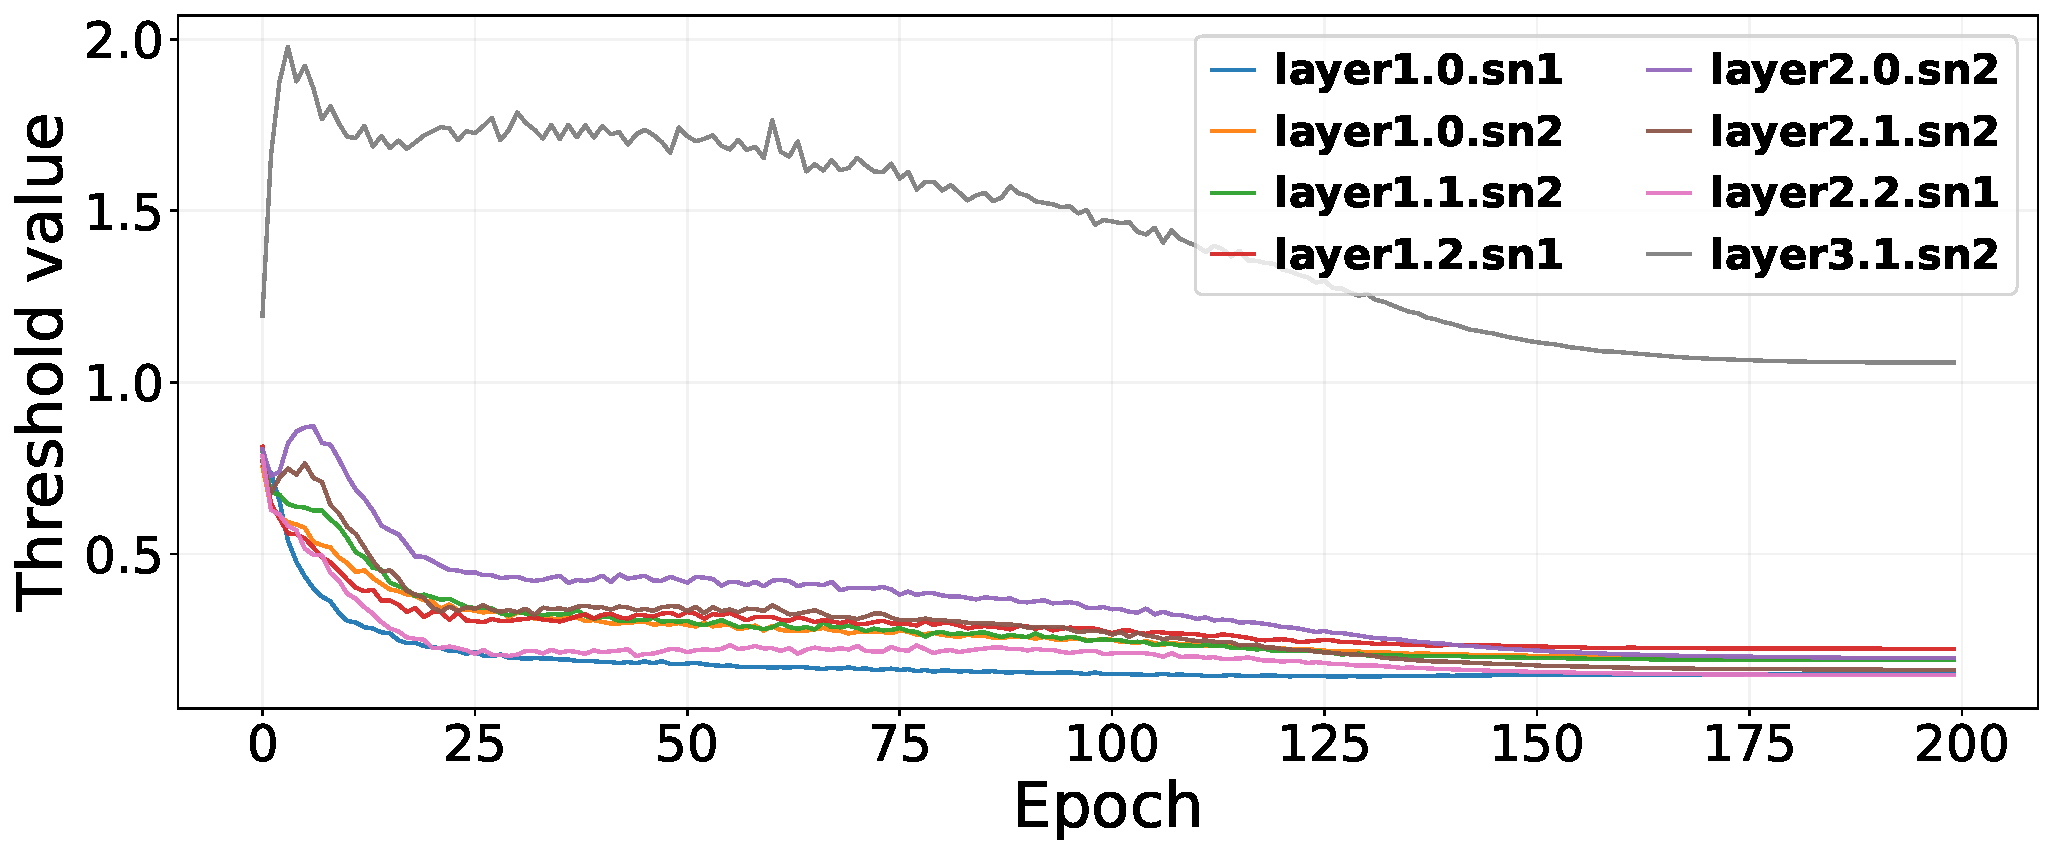
\includegraphics[width=\linewidth]{fig/threshold_training_cifar100.pdf}
    \caption{ResNet-19, CIFAR-100}
  \end{subfigure}
  \hfill
  \begin{subfigure}[b]{0.32\linewidth}
    \centering
    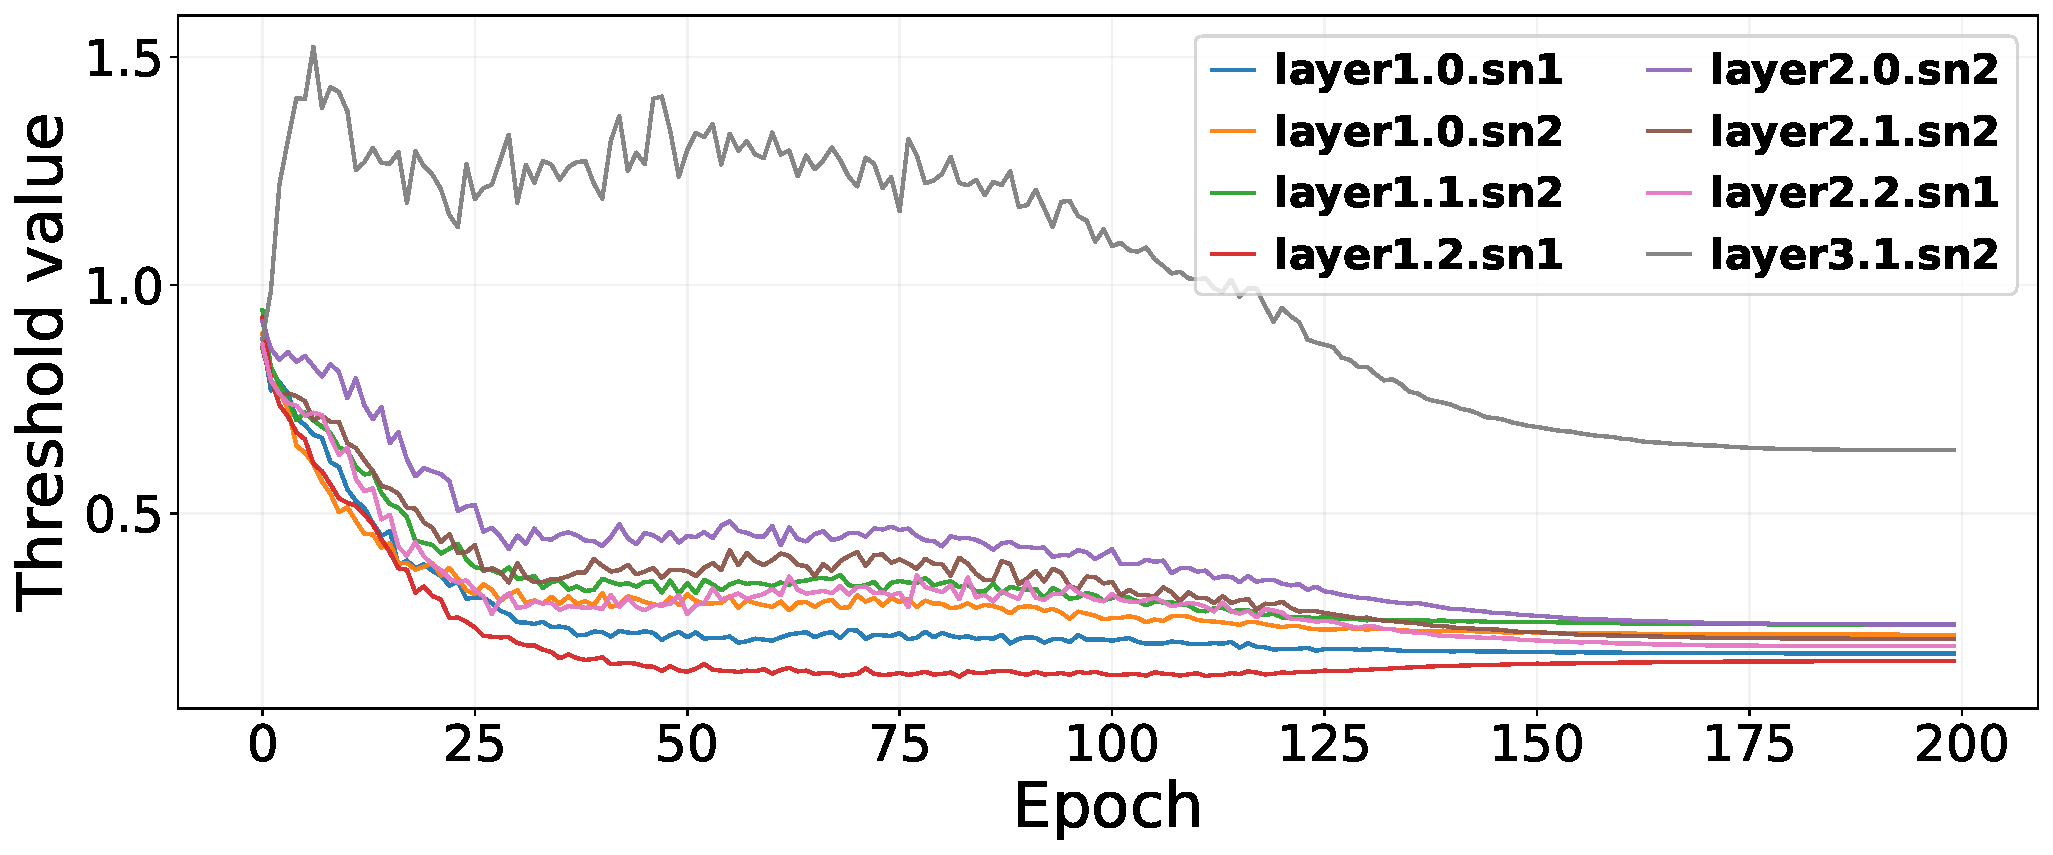
\includegraphics[width=\linewidth]{fig/threshold_training_dvscifar10.pdf}
    \caption{ResNet-19, DVS-CIFAR10}
  \end{subfigure}
  \hfill
  \begin{subfigure}[b]{0.32\linewidth}
    \centering
    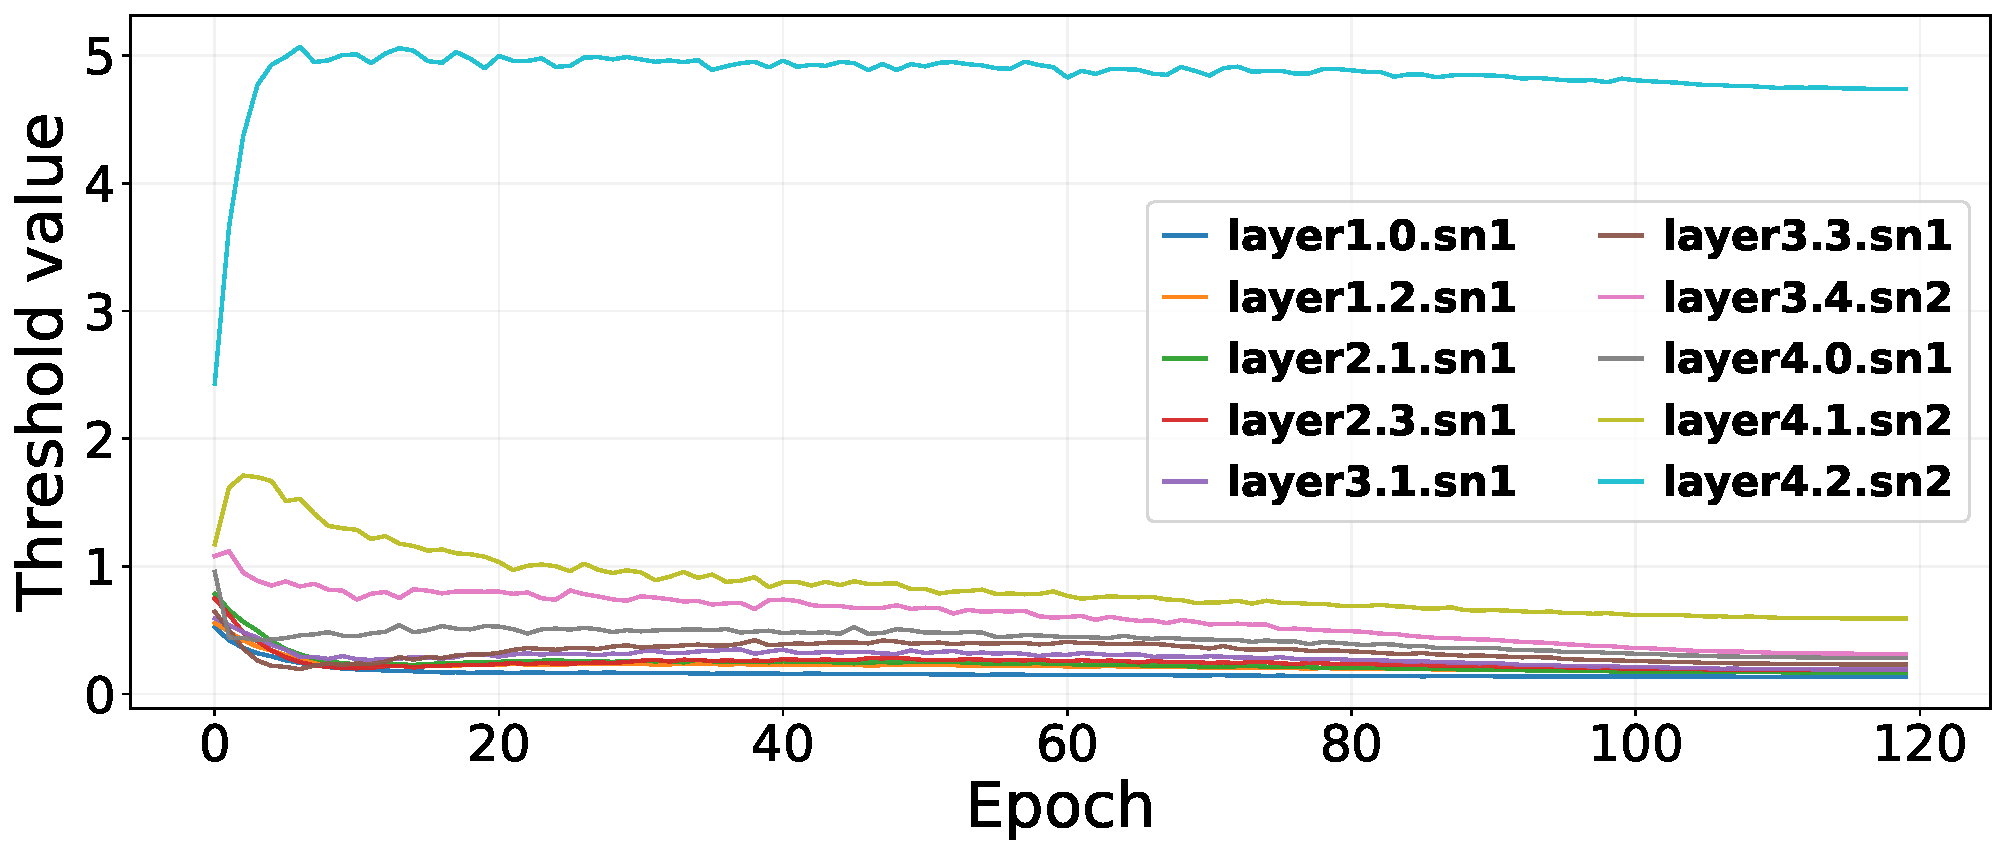
\includegraphics[width=\linewidth]{fig/threshold_training_imagenet.pdf}
    \caption{ResNet-34, ImageNet}
  \end{subfigure}
  \caption{\textbf{Trajectories of trainable $V_{\text{thr}}$ during training.} Early layers tend to settle at lower thresholds, while late or deep layers move toward larger thresholds.}
  \label{fig:vthr_dynamics}
\end{figure}

\paragraph{Implications.}
\begin{itemize}[leftmargin=2em,itemsep=2pt]
    \item \Cref{tab:metrics_ref,tab:metrics_low,tab:metrics_high} explain \emph{why} TrSG is superior: it maintains moderate AbsStr, healthy RatioAG, and low GradCV—simultaneously avoiding flooding/starvation and explosion/vanishing.
    \item The threshold trajectories in \cref{fig:vthr_dynamics} show that real trainings visit the regimes where AS-SG and RS-SG break down, so threshold-robustness is not a corner case but a practical necessity.
    \item Even when $V_{\text{thr}}$ and $\tau$ are \emph{not} trained, TrSG is the best choice across thresholds (\cref{tab:no_training_results}); using TrSG is strictly beneficial, with no downside in practice.
\end{itemize}

\section{Validation on More Surrogate Functions}
\label{sec:exp_more_surrogates}

In \cref{ch:trsg} we introduced TrSG using the rectangular surrogate as the primary example. \Cref{sec:exp_trsg} extended the experiments to the triangular surrogate. We now demonstrate TrSG's generality by evaluating it with the Arctan-based~\cite{fang:2021} and Sigmoid-based~\cite{wu:2018} surrogates while varying the initial threshold $V_{\text{thr}}$.

\paragraph{Arctan surrogate.}
The derivative of the Arctan-based surrogate is
\begin{equation}
\frac{\partial f_{sr}(x)}{\partial x}
\;=\;
\frac{\gamma}{2\bigl(1+(\tfrac{\pi}{2}\,\gamma\,x)^{2}\bigr)}.
\end{equation}

\paragraph{Sigmoid surrogate.}
The derivative of the Sigmoid-based surrogate is
\begin{equation}
\frac{\partial f_{sr}(x)}{\partial x}
\;=\;
\frac{1}{\gamma}\cdot\frac{e^{x/\gamma}}{(1+e^{x/\gamma})^{2}}.
\end{equation}
Here $\gamma$ is the steepness parameter. As before, we compare AS-SG, RS-SG, and TrSG under both soft and hard reset.

\Cref{fig:acc_different_thr_atan_sig} shows that TrSG consistently outperforms AS-SG and RS-SG under both Arctan and Sigmoid surrogates, regardless of the initial threshold. Together with the rectangular and triangular results of \cref{sec:exp_trsg}, this confirms that TrSG's threshold-robustness extends across all common surrogate-gradient shapes.

\begin{figure}[h]
  \centering
  \begin{subfigure}{0.99\linewidth}
    \centering
    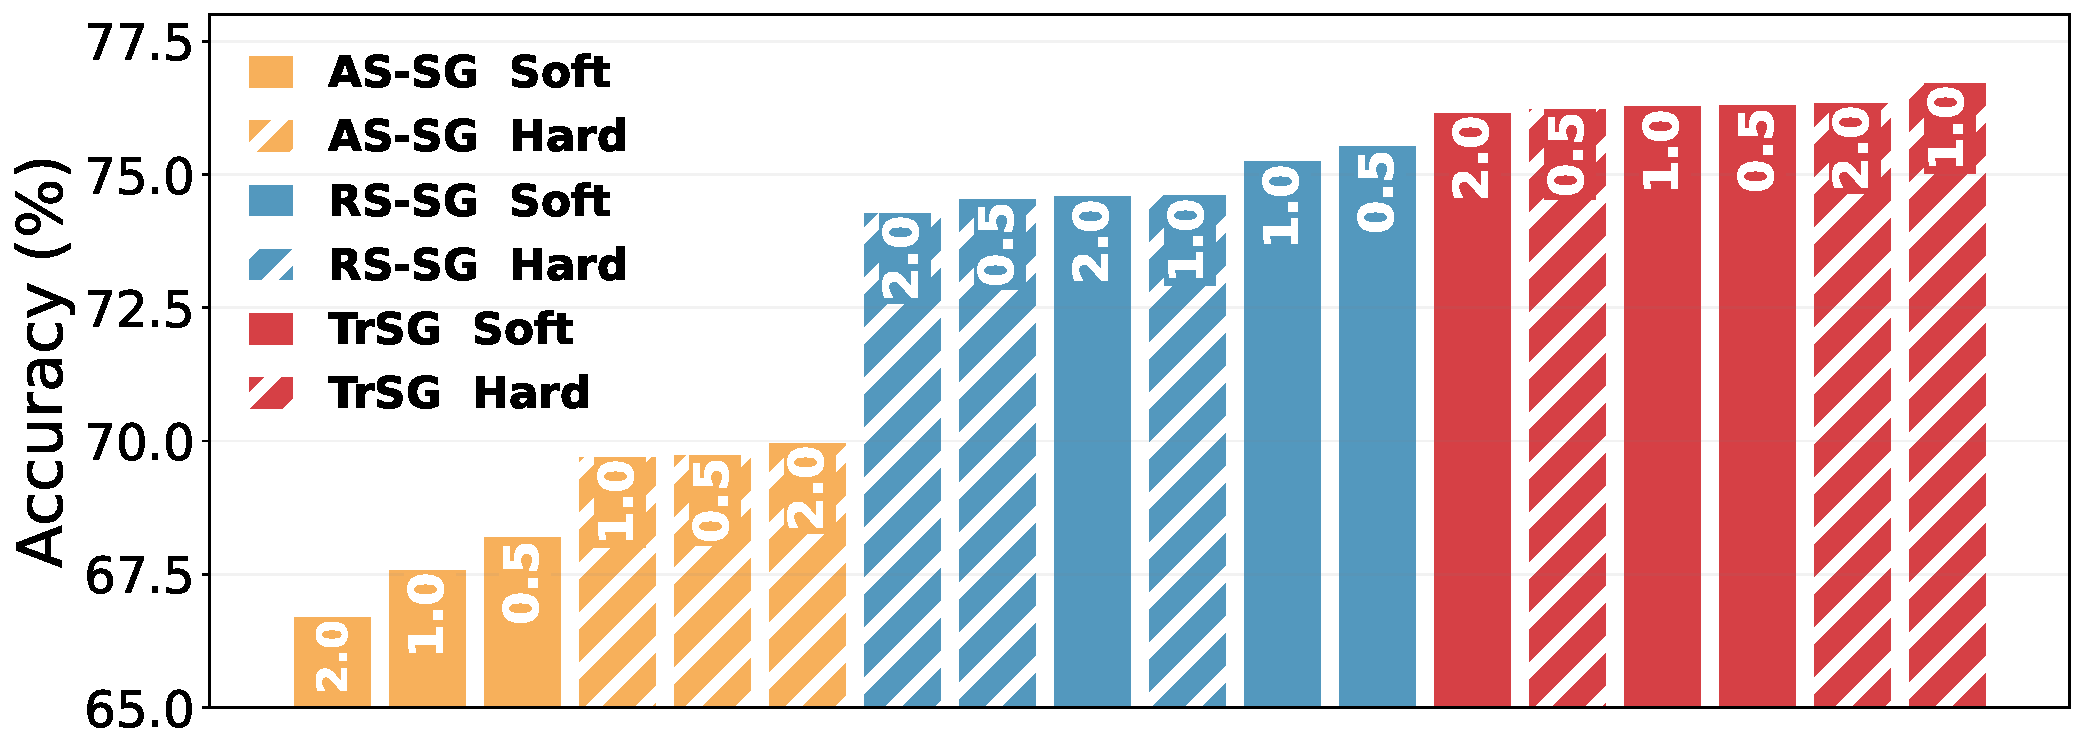
\includegraphics[width=0.99\linewidth]{fig/acc_different_thr_atan.pdf}
    \caption{Arctan surrogate}
  \end{subfigure}
  \par\medskip
  \begin{subfigure}{0.99\linewidth}
    \centering
    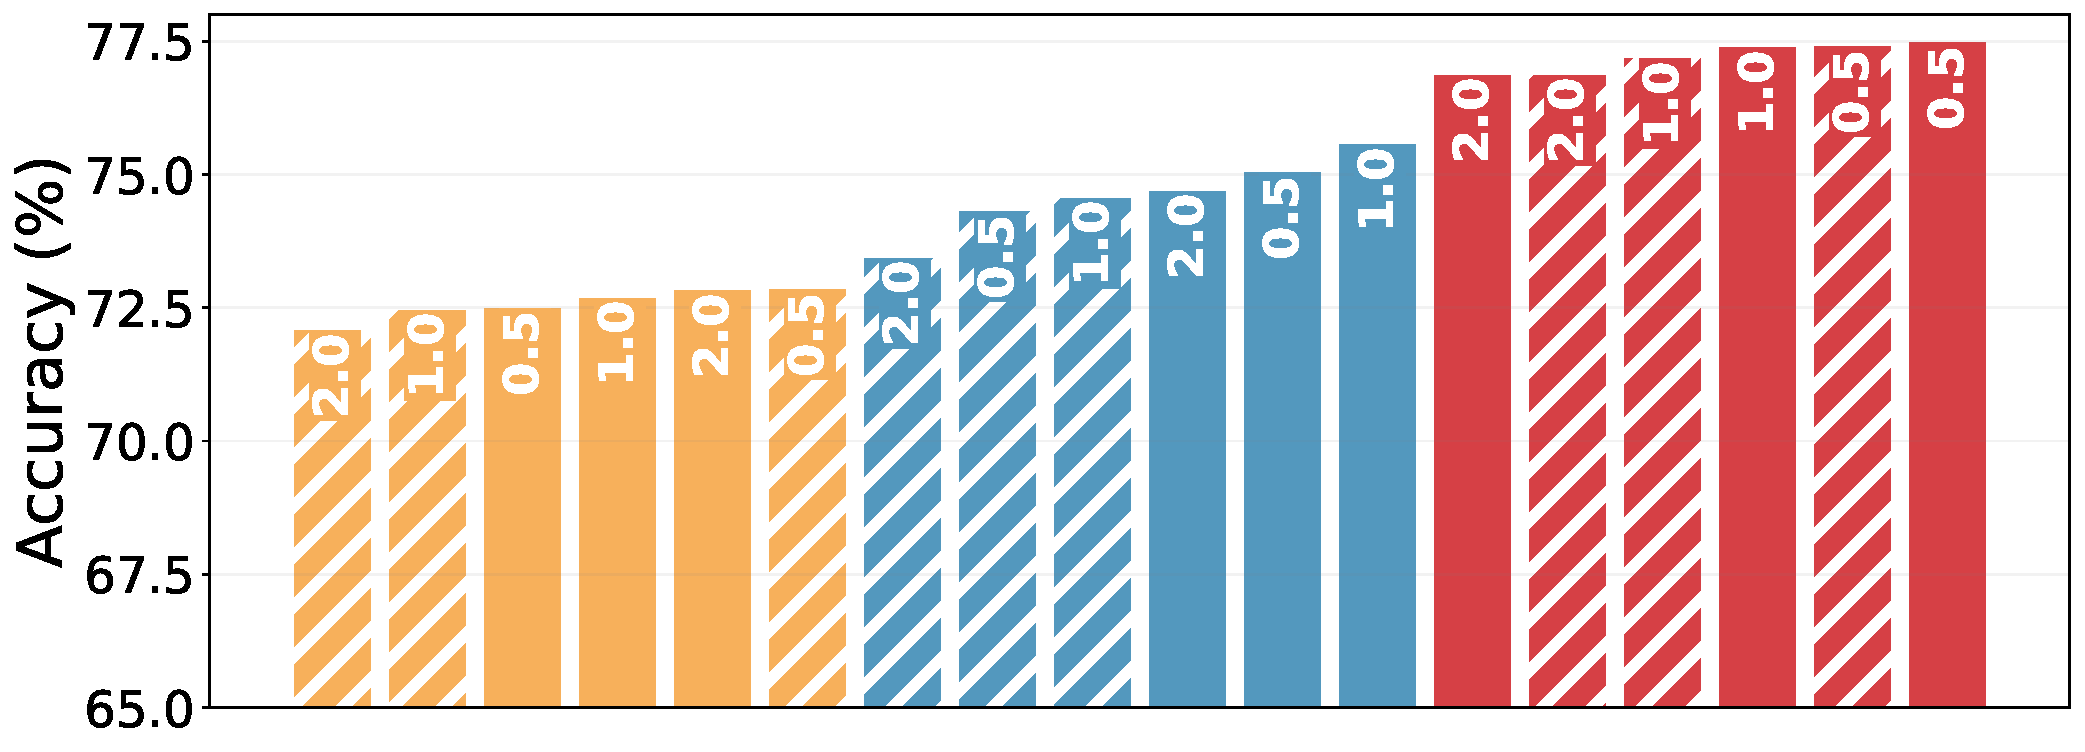
\includegraphics[width=0.99\linewidth]{fig/acc_different_thr_sigmoid.pdf}
    \caption{Sigmoid surrogate}
  \end{subfigure}
  \caption{\textbf{Accuracy under different initial $V_{\text{thr}}\in\{0.5,1.0,2.0\}$ for Arctan and Sigmoid surrogates ($\tau=2.0$).} We compare AS-SG, RS-SG, and TrSG on ResNet-19 (CIFAR-100, $T=4$), evaluating both soft- and hard-reset LIF neurons.}
  \label{fig:acc_different_thr_atan_sig}
\end{figure}

\section{Varying Initial \texorpdfstring{$\tau$}{tau} with a Fixed Initial \texorpdfstring{$V_{\text{thr}}$}{V\_thr}}
\label{sec:exp_varying_tau}

To complement the experiments in \cref{sec:exp_trsg,sec:exp_more_surrogates} (which varied $V_{\text{thr}}$), we now fix $V_{\text{thr}}=1.0$ and vary the initial leakage constant $\tau\in\{1.33,2.0,3.0\}$. \Cref{fig:acc_different_tau_all} reports accuracy across all four surrogate shapes—rectangular, triangular, Arctan, and Sigmoid—each evaluated with both soft and hard resets. Across every configuration, TrSG consistently outperforms AS-SG and RS-SG, maintaining high accuracy regardless of the initial $\tau$ and reaffirming the robustness observed under varying $V_{\text{thr}}$.

\begin{figure}[h]
  \centering
  \begin{subfigure}{0.49\linewidth}
    \centering
    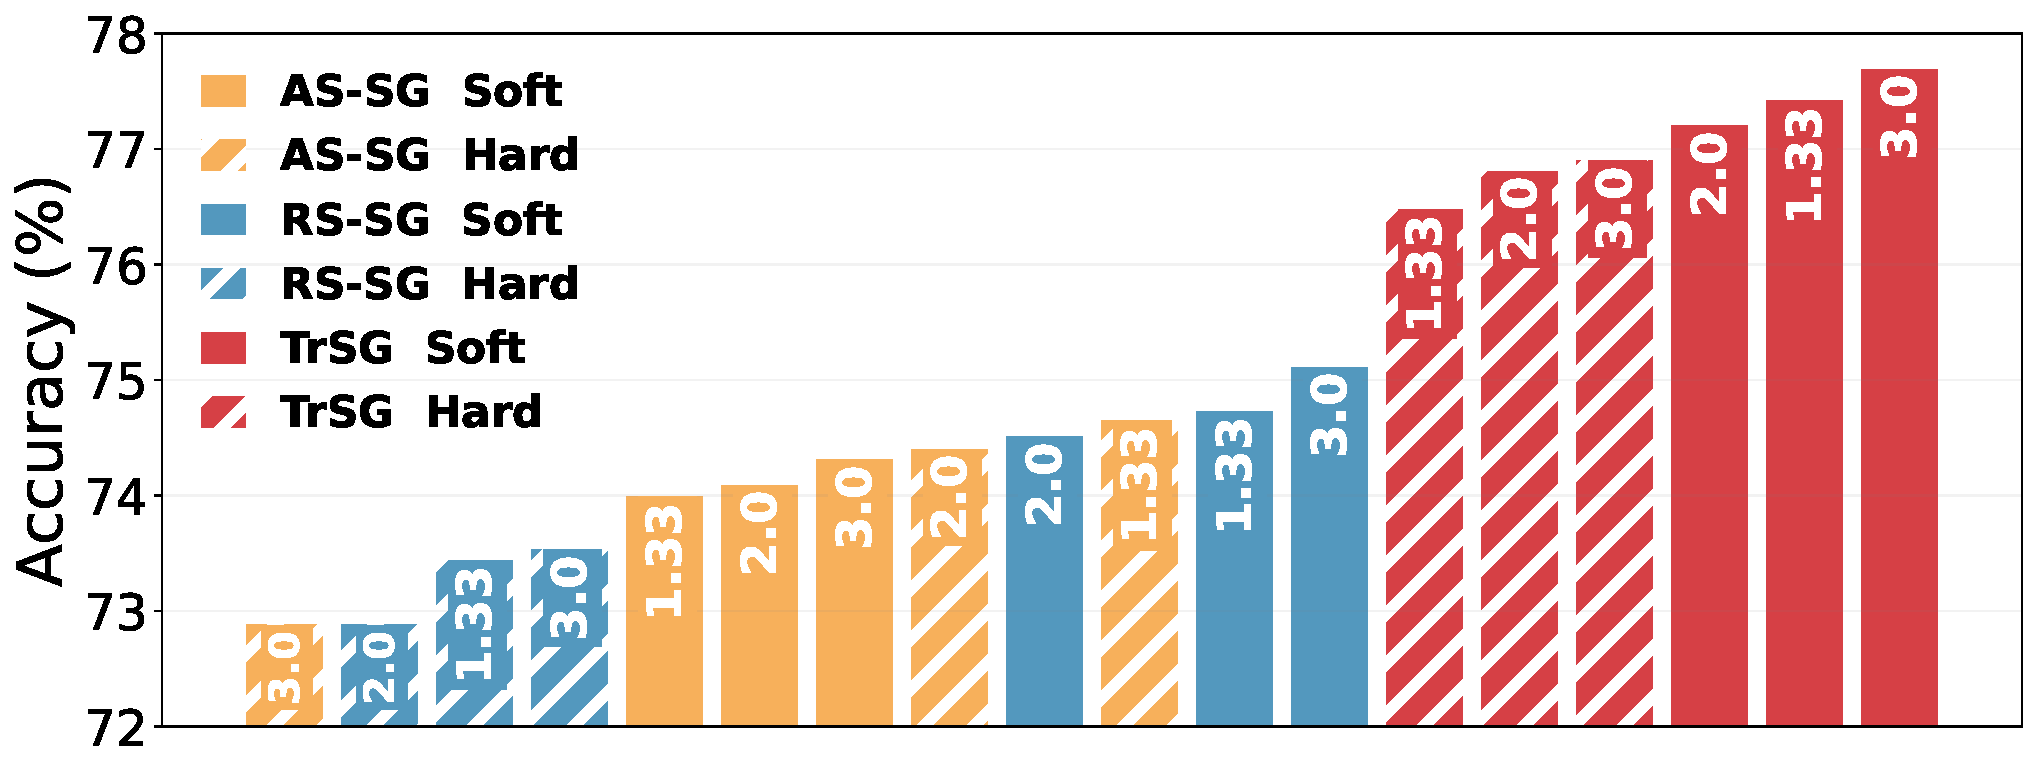
\includegraphics[width=0.99\linewidth]{fig/acc_different_tau_rect.pdf}
    \caption{Rectangular}
    \label{fig:acc_different_tau_rect}
  \end{subfigure}
  \hfill
  \begin{subfigure}{0.49\linewidth}
    \centering
    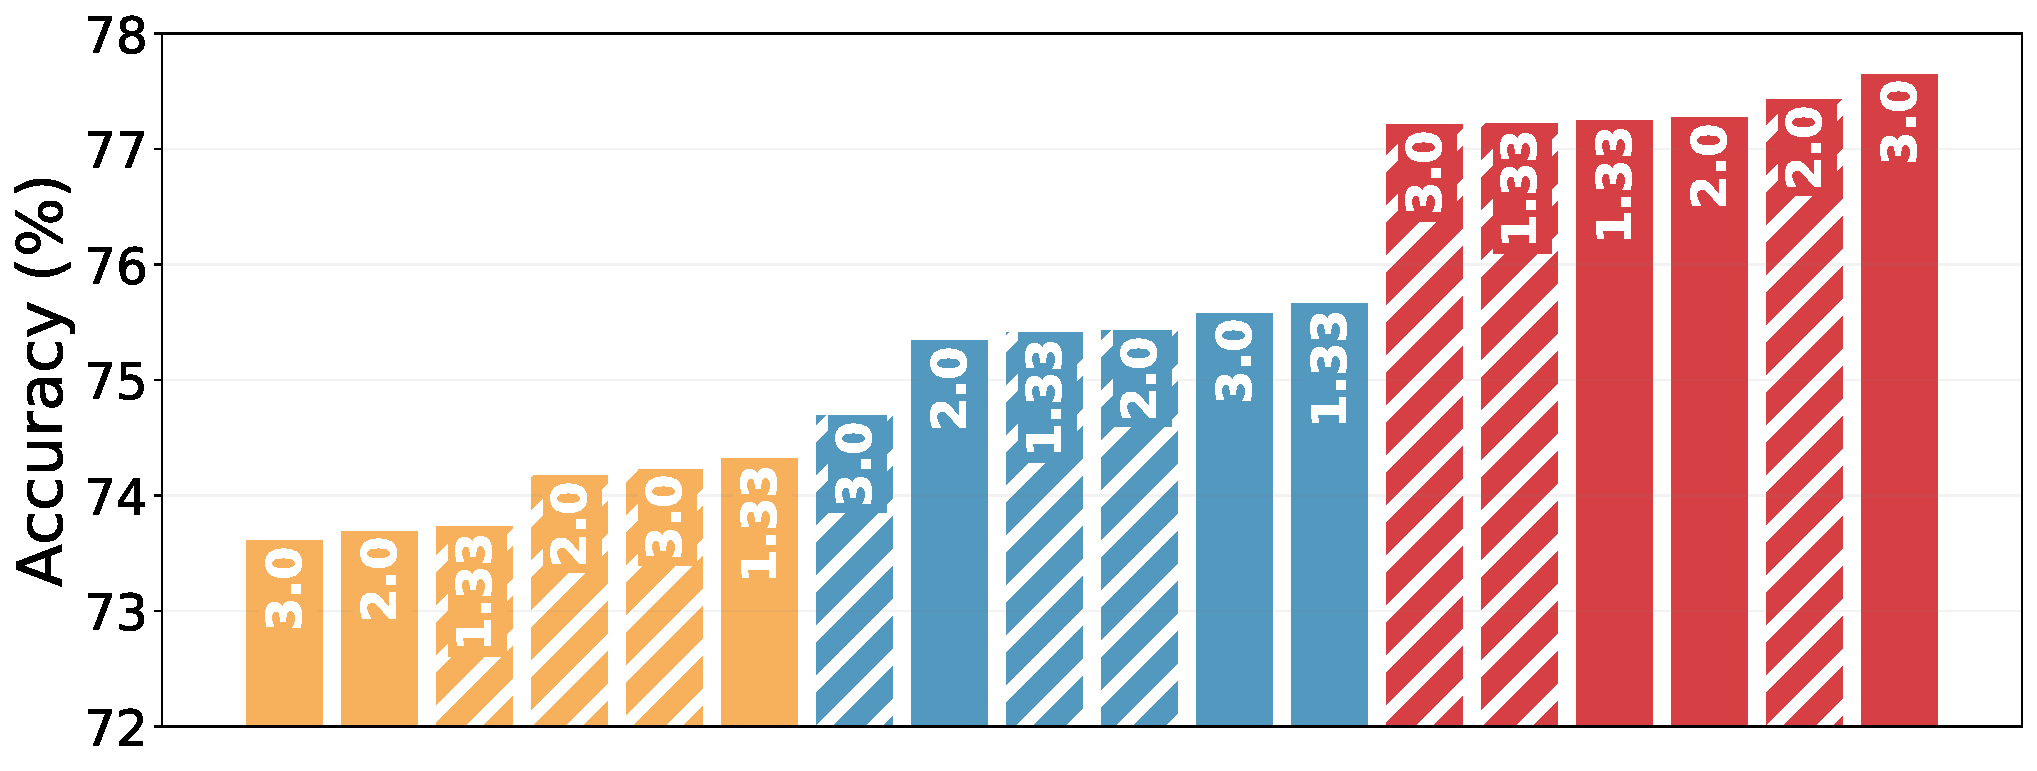
\includegraphics[width=0.99\linewidth]{fig/acc_different_tau_tri.pdf}
    \caption{Triangular}
    \label{fig:acc_different_tau_tri}
  \end{subfigure}
  \par\medskip
  \begin{subfigure}{0.49\linewidth}
    \centering
    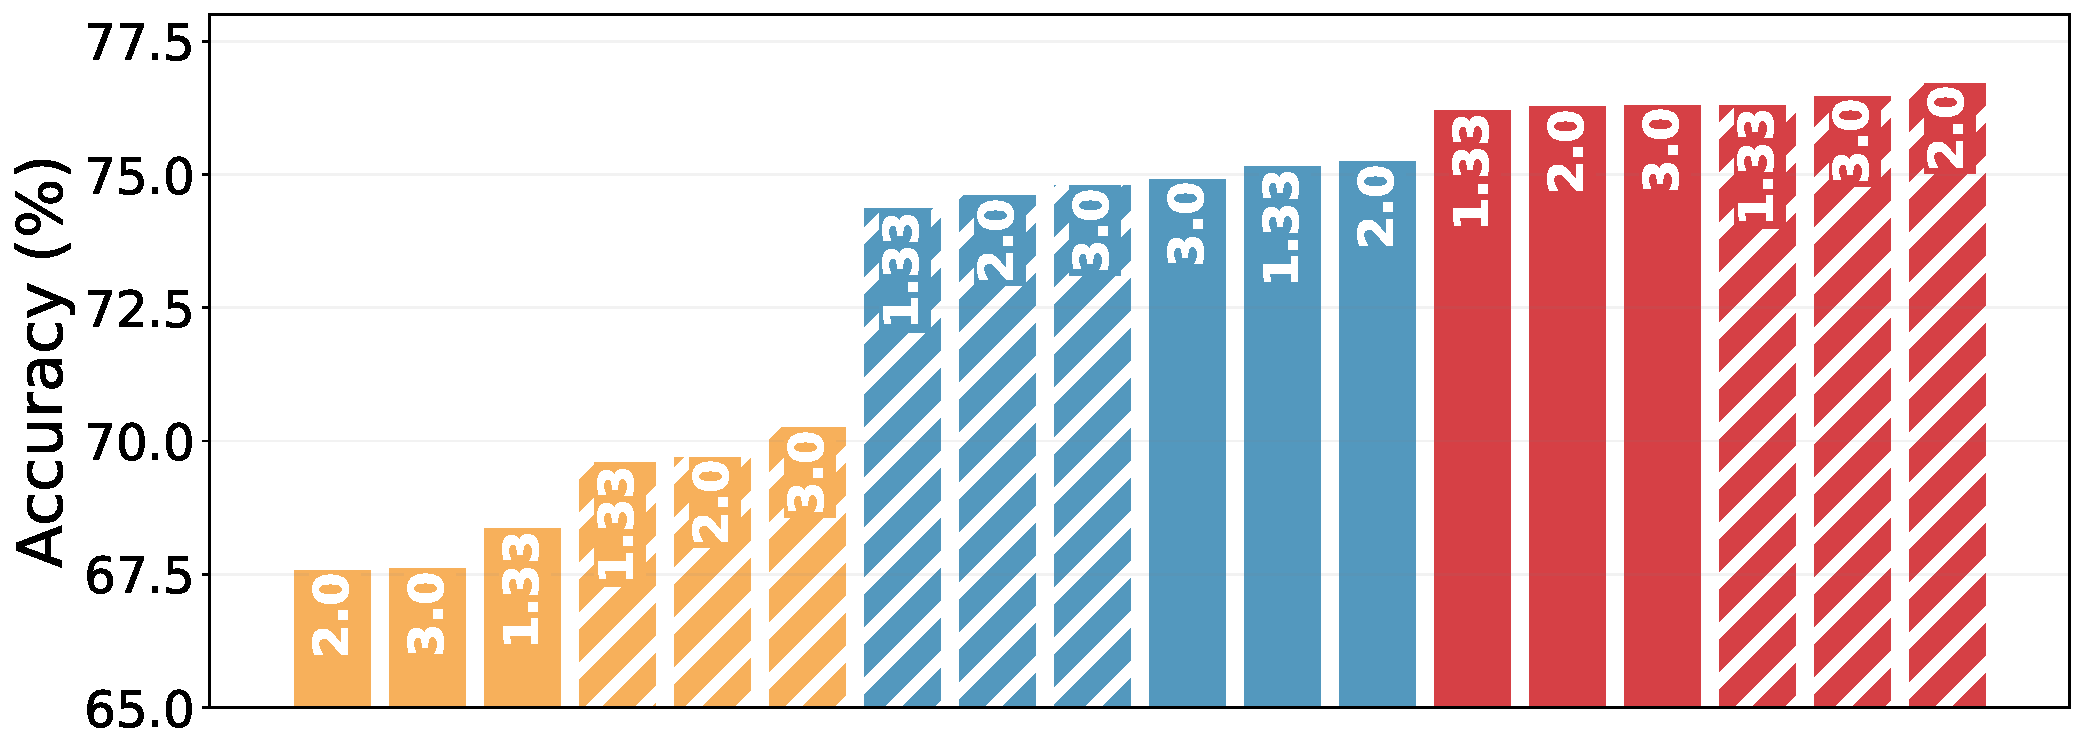
\includegraphics[width=0.99\linewidth]{fig/acc_different_tau_atan.pdf}
    \caption{Arctan}
    \label{fig:acc_different_tau_atan}
  \end{subfigure}
  \hfill
  \begin{subfigure}{0.49\linewidth}
    \centering
    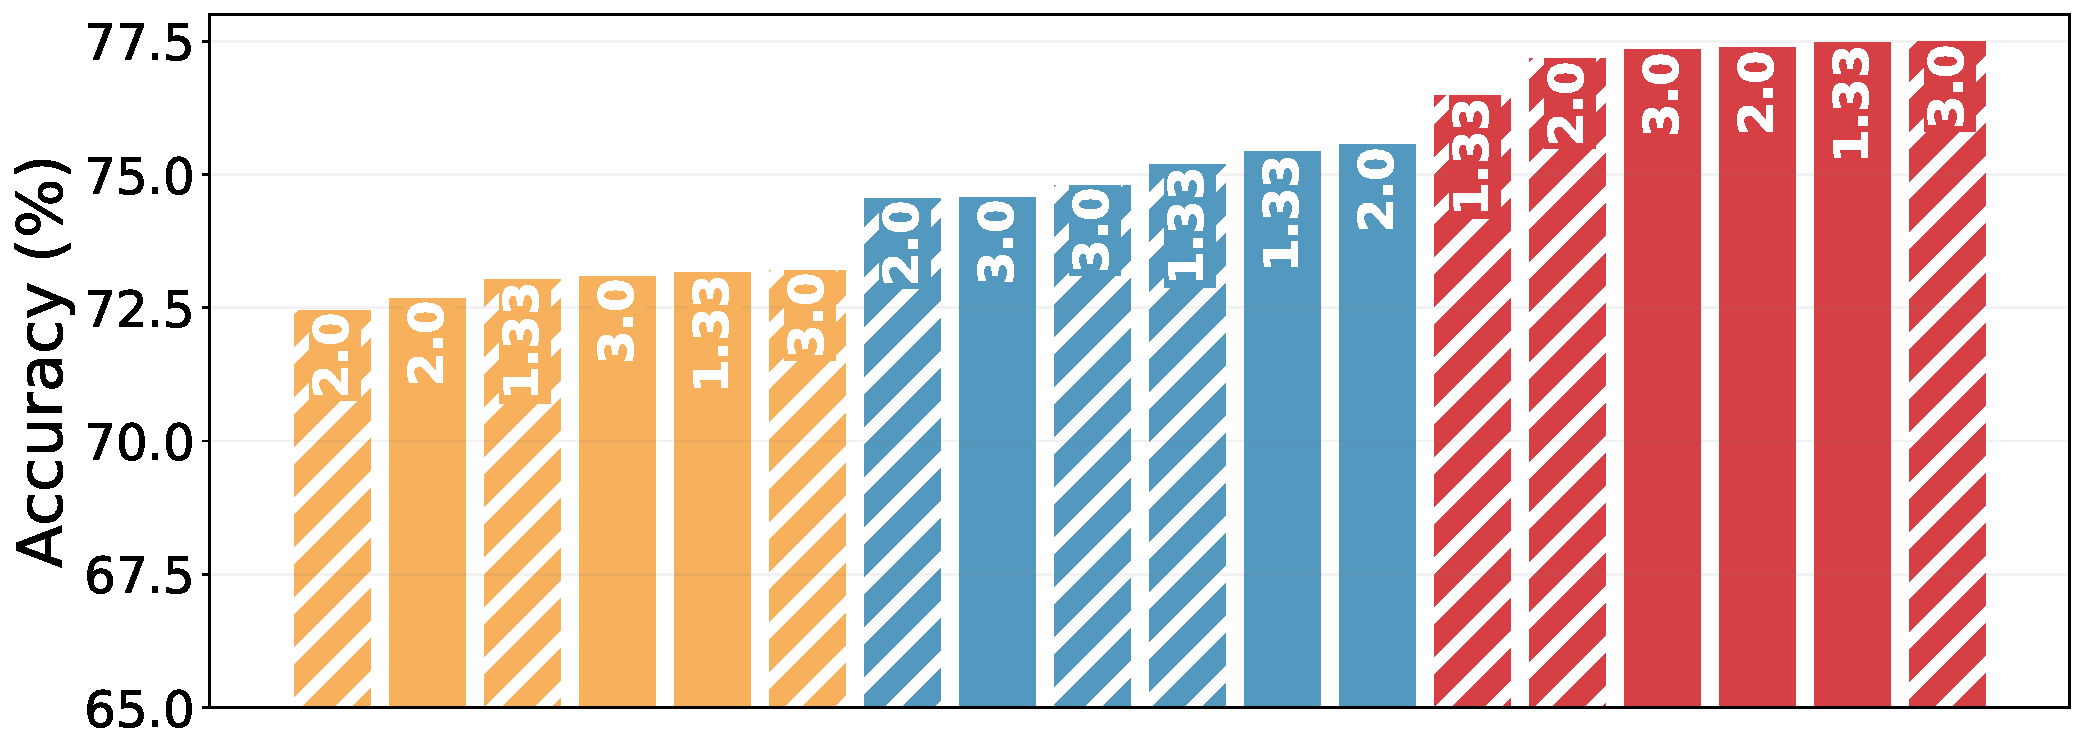
\includegraphics[width=0.99\linewidth]{fig/acc_different_tau_sigmoid.pdf}
    \caption{Sigmoid}
    \label{fig:acc_different_tau_sigmoid}
  \end{subfigure}
  \caption{\textbf{Accuracy under different initial $\tau\in\{1.33,2.0,3.0\}$ with $V_{\text{thr}}=1.0$, across all four surrogate shapes.} (a) Rectangular, (b) triangular, (c) Arctan, (d) Sigmoid—each evaluated with both soft and hard resets. ResNet-19 on CIFAR-100, $T=4$. TrSG consistently outperforms AS-SG and RS-SG in every panel.}
  \label{fig:acc_different_tau_all}
\end{figure}

\section{Impact of Trainable Parameters on Accuracy}
\label{sec:exp_trainable_impact}

To analyze the impact of training the threshold $V_{\text{thr}}$ and the leakage constant $\tau$, we run an ablation study (\cref{tab:trainable_ablation}). Training only $\tau$ slightly degrades accuracy compared with fixed parameters. Training only $V_{\text{thr}}$ yields a noticeable improvement. Training both jointly produces the best result ($77.22\%$). Although $\tau$ alone is not beneficial, its effect becomes synergistic when combined with $V_{\text{thr}}$ training: the network jointly adapts the integration time and the firing threshold to balance convergence speed and stability.

\begin{table}[h]
\centering
\small
\begin{tabular}{ccc}
\toprule
$\boldsymbol{\tau}$ \textbf{trainable} & $\boldsymbol{V_{\text{thr}}}$ \textbf{trainable} & \textbf{Accuracy (\%)} \\
\midrule
\ding{55} & \ding{55} & 75.56 \\
\ding{51} & \ding{55} & 74.61 \\
\ding{55} & \ding{51} & 76.98 \\
\ding{51} & \ding{51} & \textbf{77.22} \\
\bottomrule
\end{tabular}
\caption{Ablation of trainable internal LIF parameters on ResNet-19, CIFAR-100, $T=4$. Initial values are $V_{\text{thr}}=1.0$ and $\tau=2.0$.}
\label{tab:trainable_ablation}
\end{table}

\section{Ablation on Advanced Architecture}
\label{sec:exp_qkformer_ablation}

We further ablate the surrogate-gradient choice on a large-scale Transformer SNN, QKFormer~\cite{zhou:2024_2}, using the official training protocol while keeping all settings fixed and changing only the SG variant (\cref{tab:qkformer_ablation}). With MP-Init enabled across the board, TrSG is the only variant that reliably improves over the baseline ($+1.10$\,\%pt). AS-SG underperforms ($-1.71$\,\%pt) and RS-SG essentially matches or slightly underperforms ($-0.10$\,\%pt). These results indicate that even on advanced Transformer-based SNNs, TrSG provides consistent benefits, and that conventional SGs can in fact \emph{degrade} performance—underscoring TrSG as the safer and superior choice for modern large-scale SNN architectures.

\begin{table}[h]
\centering
\small
\begin{tabular}{lc}
\toprule
\textbf{Method} & \textbf{Top-1 (\%)} \\
\midrule
QKFormer (HST-10-384)              & 78.80 \\
\quad + AS-SG                      & 77.09 \\
\quad + RS-SG                      & 78.70 \\
\quad + \textbf{TrSG}              & \textbf{79.90} \\
\bottomrule
\end{tabular}
\caption{Ablation of the surrogate-gradient choice on QKFormer (HST-10-384), ImageNet, $T=4$. All runs follow the official training recipe with only the SG variant differing. MP-Init is enabled in every case.}
\label{tab:qkformer_ablation}
\end{table}

\section{Accuracy vs.\ Firing Rate under TrSG}
\label{sec:exp_firing_rate_trsg}

\Cref{subsec:exp_pareto} showed that MP-Init forms a Pareto front over firing rate. A natural question is whether training the internal parameters $V_{\text{thr}}$ and $\tau$ with TrSG merely increases spike counts to boost accuracy. To decouple these effects, we sweep the same sparsity regularization loss~\cite{yan:2022} as before and compare \emph{Training} (TrSG updates $V_{\text{thr}}$ and $\tau$) against \emph{No Training} (both frozen).

As shown in \cref{fig:firing_rate_vs_accuracy_trsg}, the Training curve strictly dominates the No-Training curve at all firing rates, indicating that TrSG's improvement stems from well-adapted neuron dynamics rather than excessive spiking. This is consistent with the threshold trajectories of \cref{fig:vthr_dynamics}, where layers evolve toward operating points that favor stable, informative spikes.

\begin{figure}[h]
  \centering
  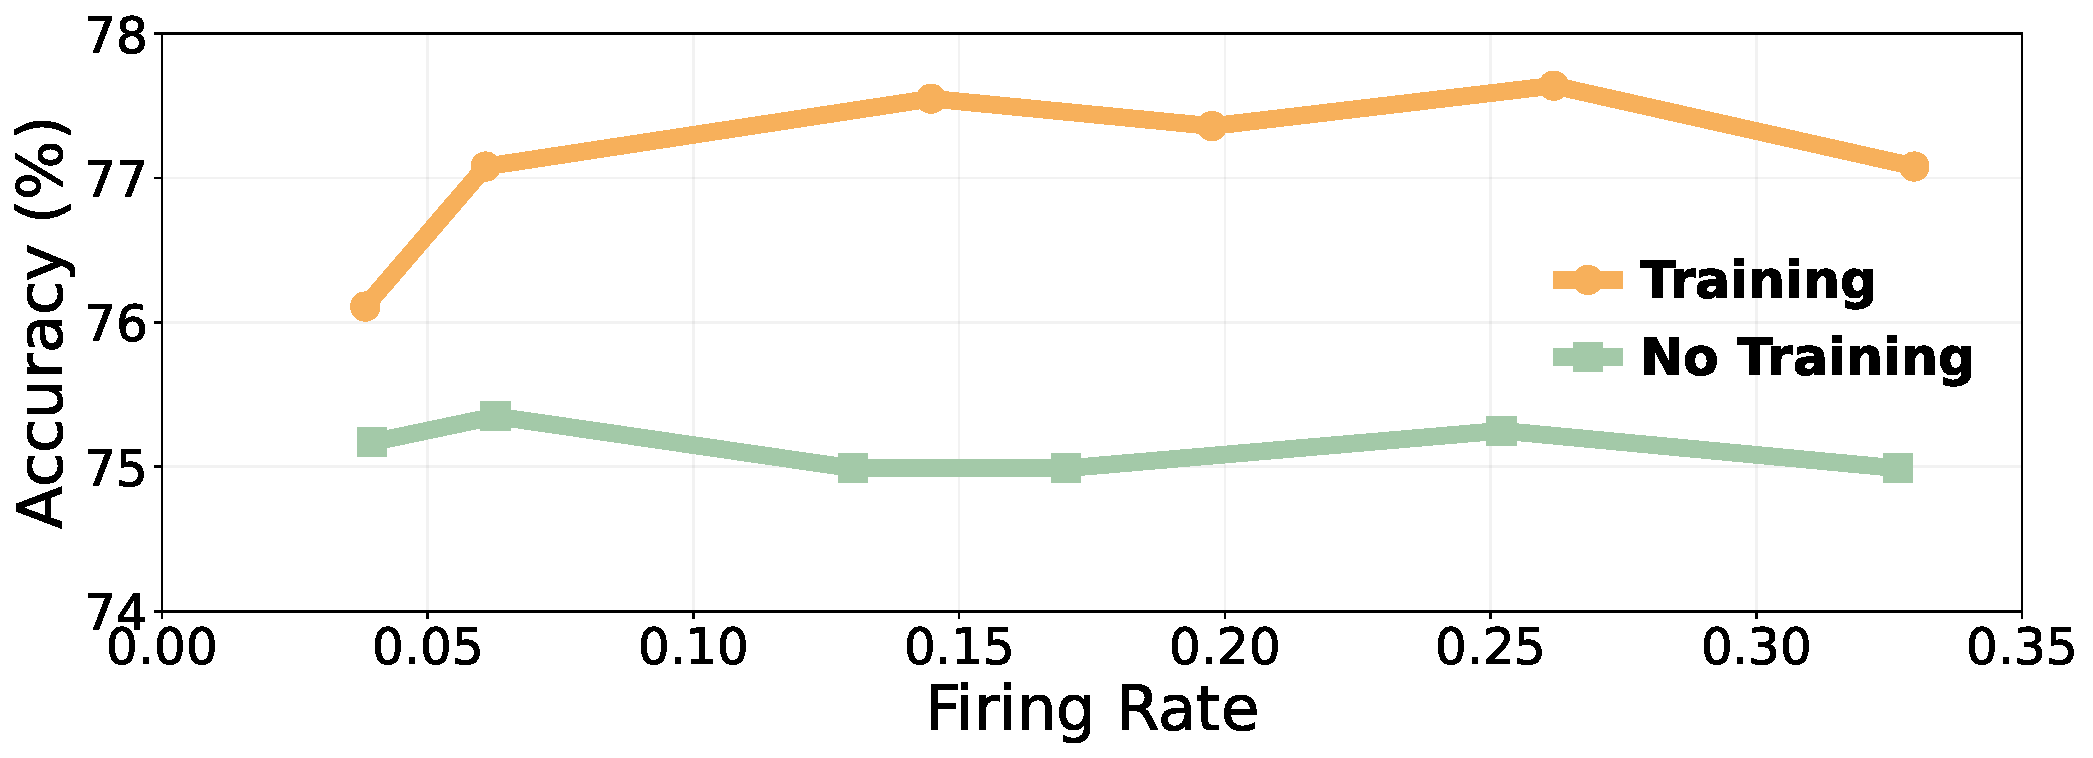
\includegraphics[width=0.85\linewidth]{fig/firing_rate_vs_accuracy_trsg.pdf}
  \caption{\textbf{Accuracy vs.\ firing rate under TrSG.} We sweep a sparsity loss~\cite{yan:2022} to match global firing rates and compare \emph{Training} (learn $V_{\text{thr}}$ and $\tau$ with TrSG) against \emph{No Training} (both frozen).}
  \label{fig:firing_rate_vs_accuracy_trsg}
\end{figure}

\section{Energy Cost}
\label{sec:exp_energy}

Since the firing rate tightly correlates with accumulate operations (ACs)—and therefore energy—the analyses in \cref{subsec:exp_pareto,sec:exp_firing_rate_trsg} can be viewed as an energy--accuracy trade-off. To quantify this, we measure ACs and multiply--accumulate operations (MACs) and compute the corresponding energy following~\cite{energy}; \cref{tab:energy_calculation} reports the result. At similar firing rates (and hence similar energy cost), training the internal neuron parameters with TrSG yields consistently higher accuracy. In short, TrSG improves accuracy at nearly the same energy cost—the gains come from better adaptation of $V_{\text{thr}}$ and $\tau$, not from increasing spike counts.

\begin{table}[h]
\centering
\small
\begin{tabular}{ccccc}
\toprule
\textbf{MP-Init} & \textbf{TrSG} & \textbf{ACs / MACs (G)} & \textbf{Energy (mJ)} & \textbf{Acc (\%)} \\
\midrule
\ding{55} & \ding{55} & 1.03 / 0.14 & 1.57 & 75.58 \\
\ding{51} & \ding{55} & 1.01 / 0.14 & 1.57 & 76.20 \\
\ding{55} & \ding{51} & 1.13 / 0.14 & 1.68 & 77.13 \\
\ding{51} & \ding{51} & 1.12 / 0.14 & 1.67 & \textbf{77.68} \\
\bottomrule
\end{tabular}
\caption{\textbf{Energy at comparable firing rates.} Accumulate operations (ACs), multiply--accumulate operations (MACs), and computed energy cost. ResNet-19, CIFAR-100, $T=4$.}
\label{tab:energy_calculation}
\end{table}

\section{Final Values of Neuron Parameters}
\label{sec:exp_final_values}

In addition to learning the network weights, our approach optimizes the neuron parameters $V_{\text{thr}}$ and $\tau$, while MP-Init tracks an internal running mean of the membrane potential at the last timestep, $U[T]$. To investigate how these three quantities evolve through training, we visualize their final layer-wise values for both CIFAR-100 and DVS-CIFAR10 in \cref{fig:final_values}, considering soft and hard resets.

\paragraph{Running mean of $U[T]$.}
The running mean of $U[T]$ typically settles at about half of $V_{\text{thr}}$ in the soft-reset case (\cref{fig:final_values_cifar100_soft,fig:final_values_dvs_soft}) and roughly a quarter of $V_{\text{thr}}$ for hard-reset neurons (\cref{fig:final_values_cifar100_hard,fig:final_values_dvs_hard}). This indicates that the average post-synaptic potential remains below the learned threshold in most layers yet remains sufficiently high to generate spikes when needed.

\paragraph{Threshold $V_{\text{thr}}$.}
Across both datasets and reset types, the learned $V_{\text{thr}}$ commonly falls below $0.5$ in earlier and intermediate layers, suggesting that moderate thresholds facilitate stable spiking activity.

\paragraph{Decay constant $\tau$.}
We observe a consistent trend of $\tau$ converging around $1.5$--$2.0$ in most layers for CIFAR-100, while on DVS-CIFAR10, $\tau$ tends to reach larger values (e.g., near $2.5$--$3.0$). This implies that dynamic event-driven data benefit from neurons accumulating input more slowly, whereas CIFAR-100's static images favor a shorter effective integration time.

\paragraph{Last-layer behavior.}
Interestingly, in the final layer on both datasets, $\tau$ commonly drops close to $1$, effectively making it a binary layer. The layer may act as a gating mechanism, helping the model classify features decisively without excessive temporal integration.

\begin{figure}[h]
  \centering
  \begin{subfigure}{0.49\linewidth}\centering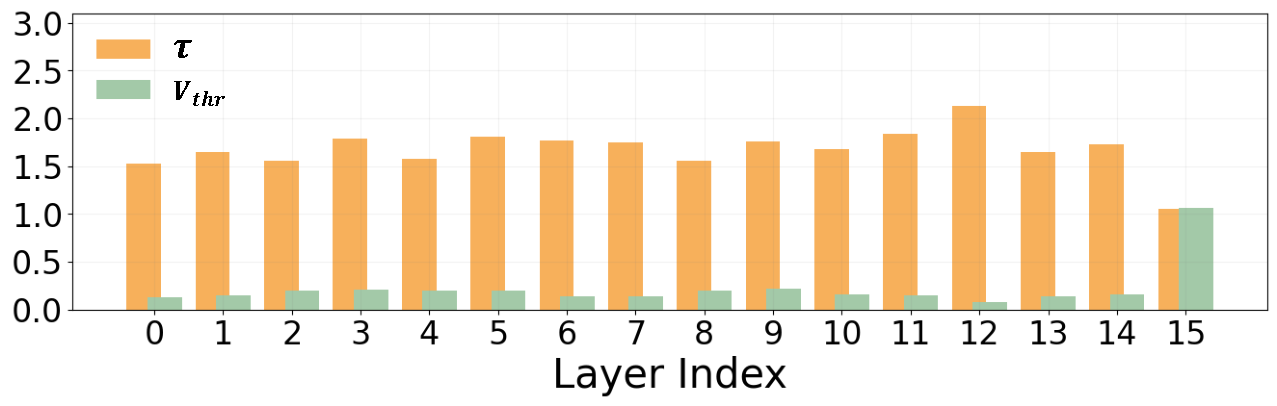
\includegraphics[width=0.99\linewidth]{fig/final_value_tau_thr_cifar100_resnet19_soft_reset_with_legend.pdf}\end{subfigure}
  \begin{subfigure}{0.49\linewidth}\centering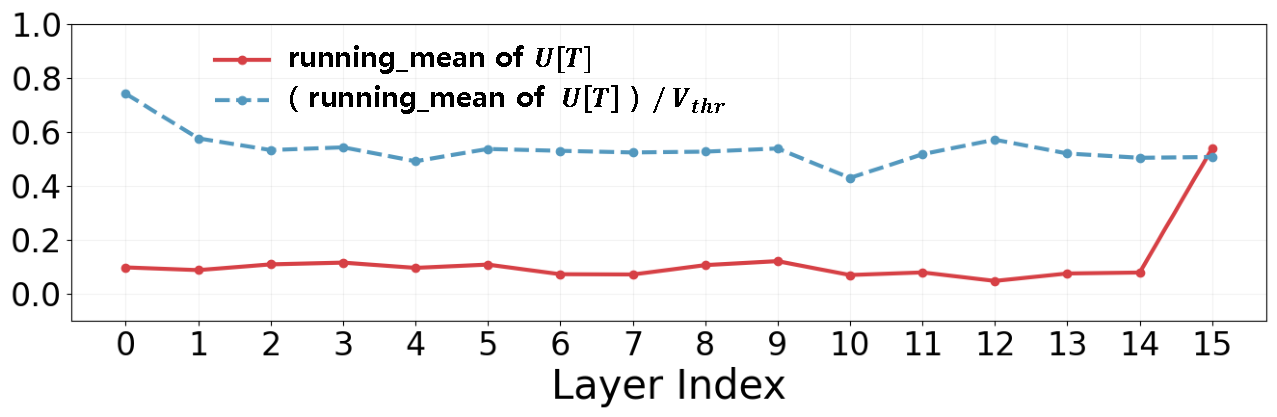
\includegraphics[width=0.99\linewidth]{fig/final_value_running_mean_cifar100_resnet19_soft_reset_with_legend.pdf}\end{subfigure}
  \par
  \begin{subfigure}{0.99\linewidth}\centering\caption{CIFAR-100 (soft reset)}\label{fig:final_values_cifar100_soft}\end{subfigure}
  \par\medskip
  \begin{subfigure}{0.49\linewidth}\centering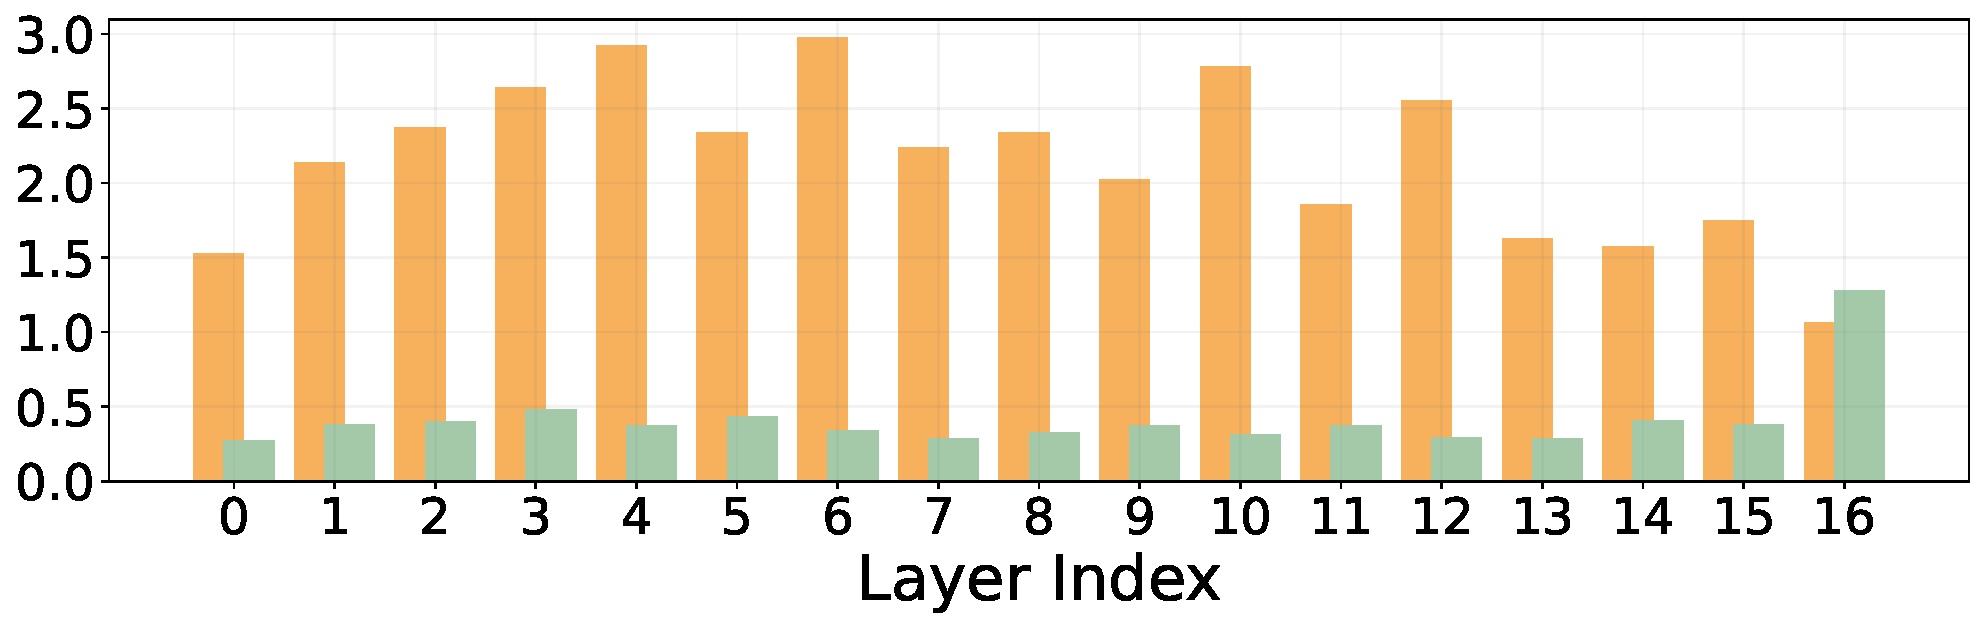
\includegraphics[width=0.99\linewidth]{fig/final_value_tau_thr_dvscifar10_resnet19_soft_reset.pdf}\end{subfigure}
  \begin{subfigure}{0.49\linewidth}\centering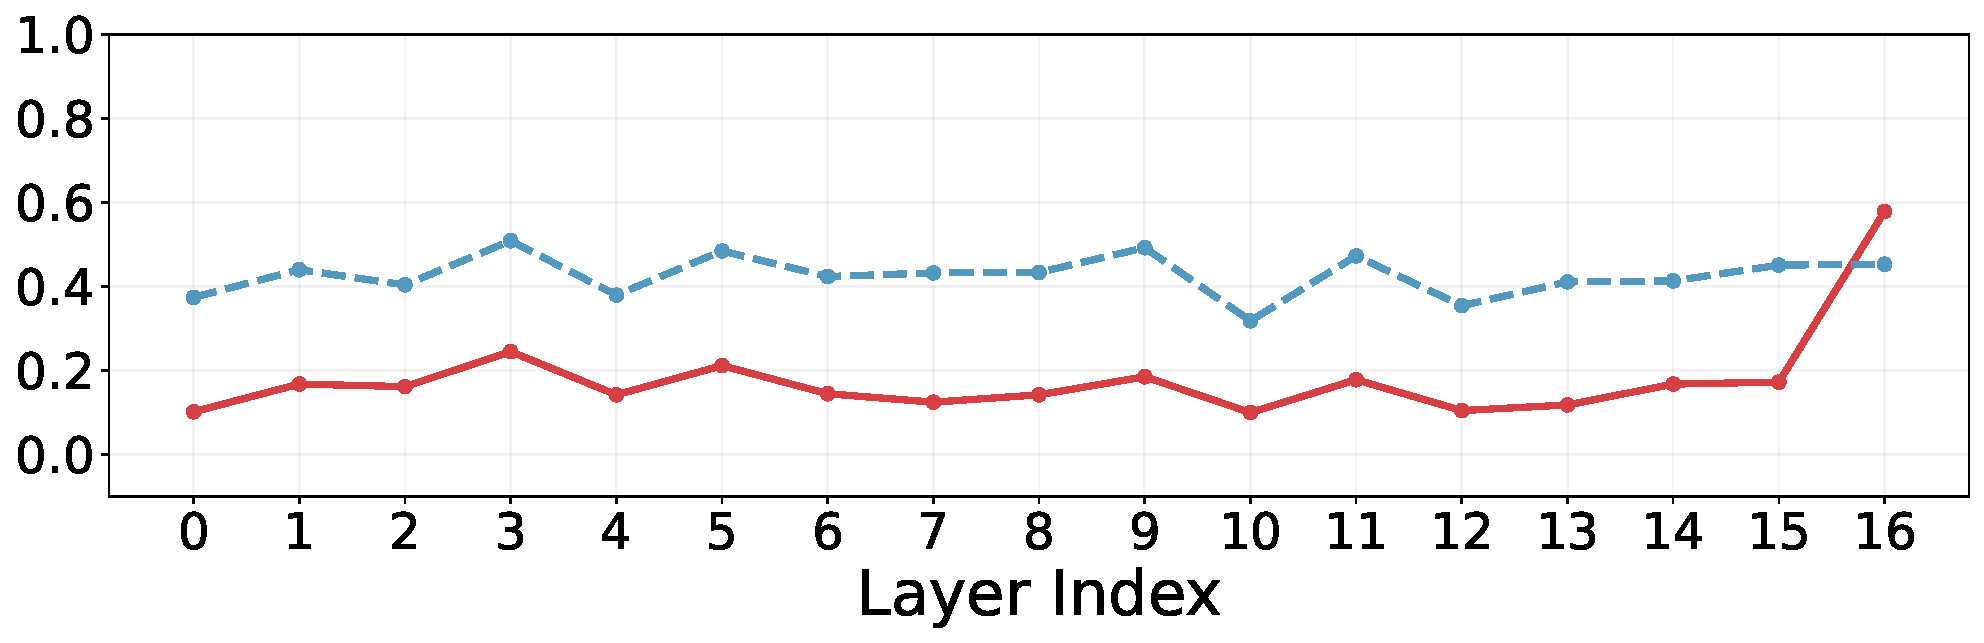
\includegraphics[width=0.99\linewidth]{fig/final_value_running_mean_dvscifar10_resnet19_soft_reset.pdf}\end{subfigure}
  \par
  \begin{subfigure}{0.99\linewidth}\centering\caption{DVS-CIFAR10 (soft reset)}\label{fig:final_values_dvs_soft}\end{subfigure}
  \par\medskip
  \begin{subfigure}{0.49\linewidth}\centering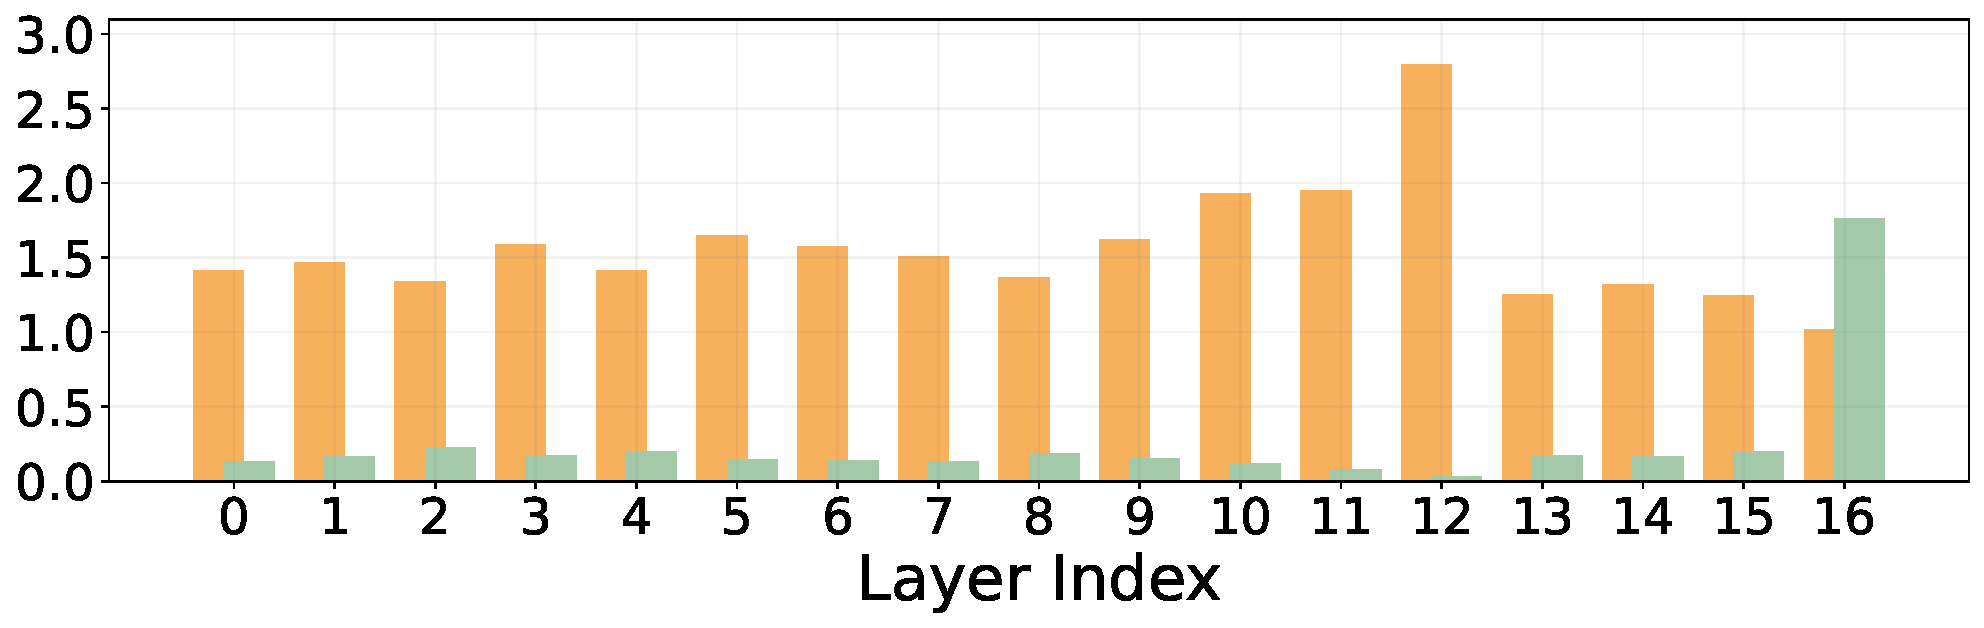
\includegraphics[width=0.99\linewidth]{fig/final_value_tau_thr_cifar100_resnet19_hard_reset.pdf}\end{subfigure}
  \begin{subfigure}{0.49\linewidth}\centering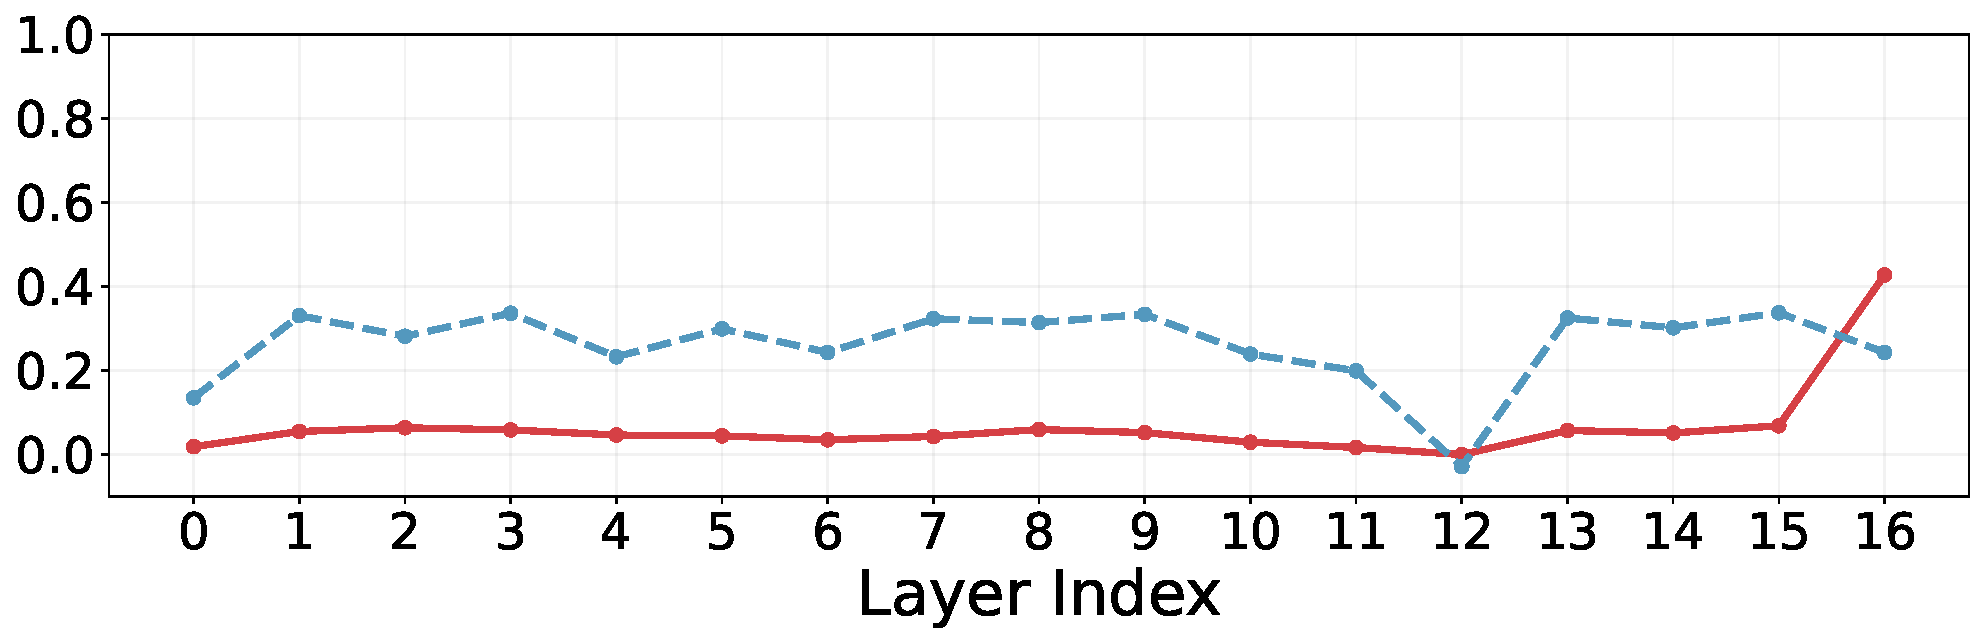
\includegraphics[width=0.99\linewidth]{fig/final_value_running_mean_cifar100_resnet19_hard_reset.pdf}\end{subfigure}
  \par
  \begin{subfigure}{0.99\linewidth}\centering\caption{CIFAR-100 (hard reset)}\label{fig:final_values_cifar100_hard}\end{subfigure}
  \par\medskip
  \begin{subfigure}{0.49\linewidth}\centering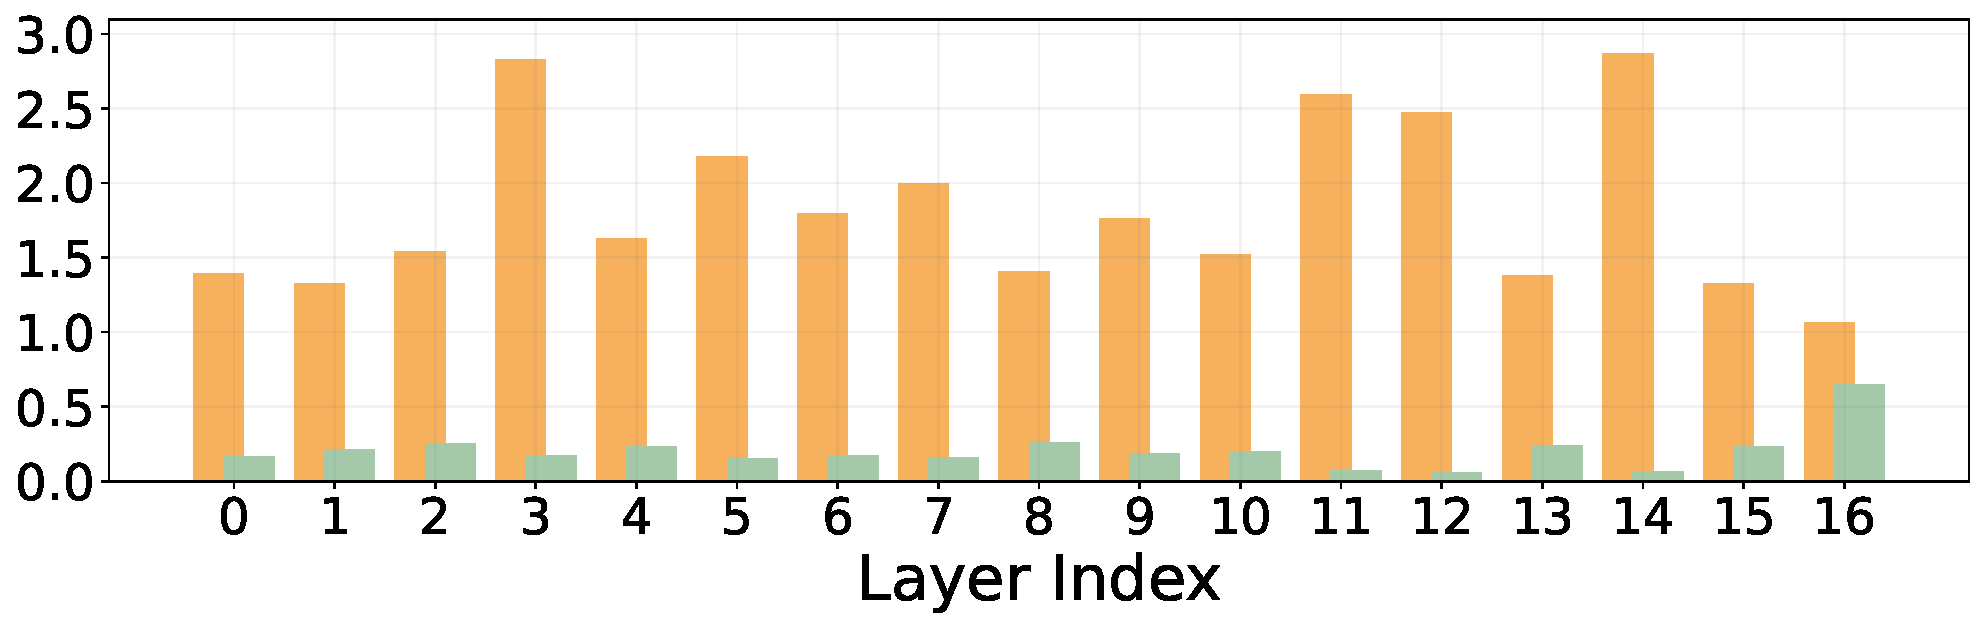
\includegraphics[width=0.99\linewidth]{fig/final_value_tau_thr_dvscifar10_resnet19_hard_reset.pdf}\end{subfigure}
  \begin{subfigure}{0.49\linewidth}\centering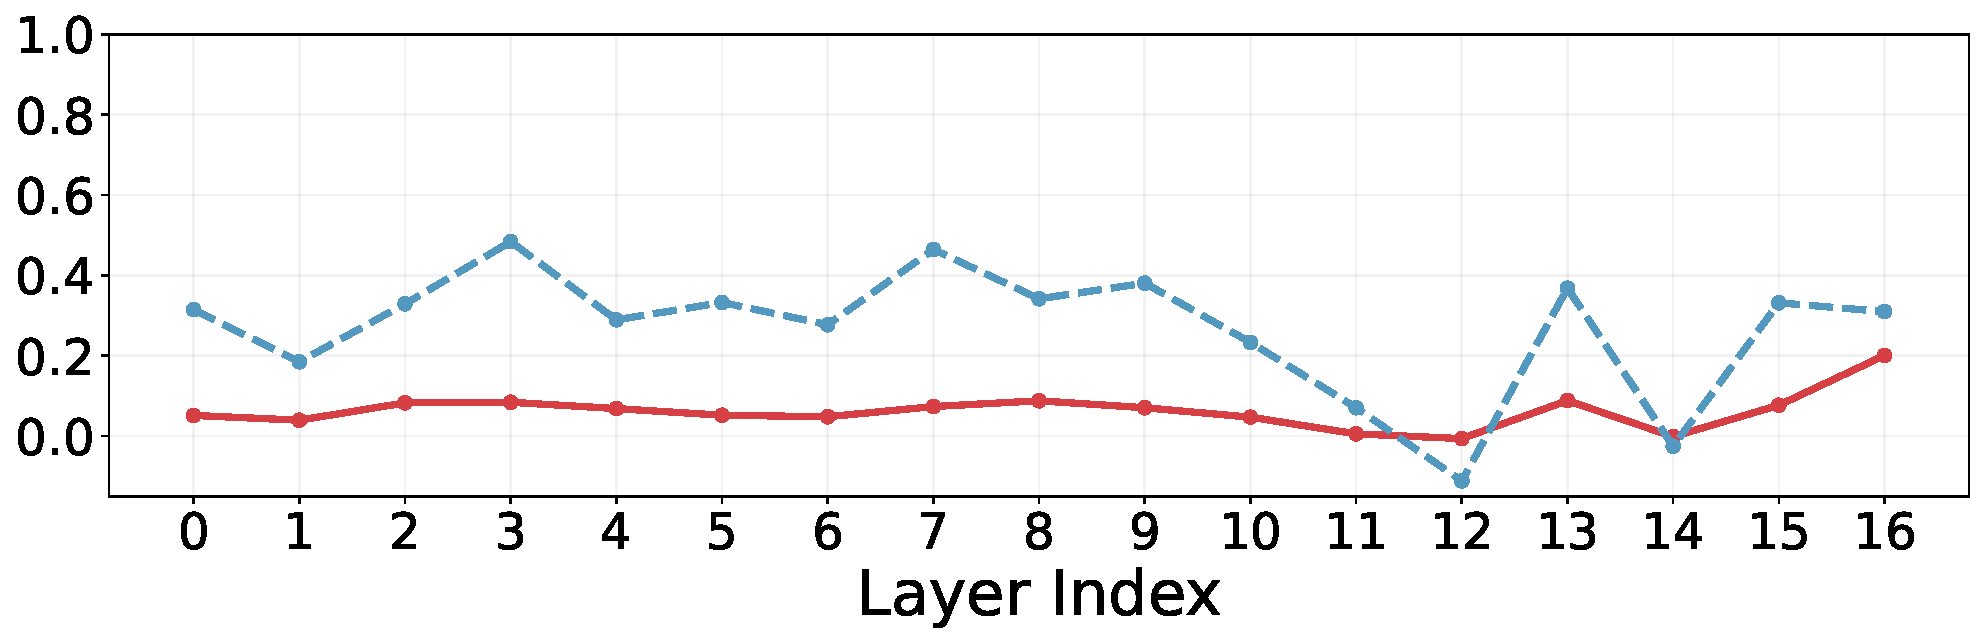
\includegraphics[width=0.99\linewidth]{fig/final_value_running_mean_dvscifar10_resnet19_hard_reset.pdf}\end{subfigure}
  \par
  \begin{subfigure}{0.99\linewidth}\centering\caption{DVS-CIFAR10 (hard reset)}\label{fig:final_values_dvs_hard}\end{subfigure}
  \caption{Final values of $V_{\text{thr}}$, $\tau$, and the running mean of $U[T]$ after training. ResNet-19 on CIFAR-100 ($T=4$) and DVS-CIFAR10 ($T=10$).}
  \label{fig:final_values}
\end{figure}

\section{Discussion}
\label{sec:exp_discussion}

The empirical results corroborate the analytical claims of \cref{ch:mpinit,ch:trsg}: MP-Init removes the residual TCS that prior normalization-based remedies miss, and TrSG removes the threshold-induced gradient pathologies that prior surrogate-gradient designs suffer from. Their effects are complementary—as evidenced by the $2$--$5$\,\%pt cumulative gain on DVS-CIFAR10—and they generalize cleanly across architectures, datasets, and downstream tasks while preserving the standard LIF inference pipeline. The stability metrics in \cref{sec:exp_trsg_impact}, the threshold trajectories in \cref{subsec:exp_threshold_trajectories}, and the converged neuron parameters in \cref{sec:exp_final_values} together provide a coherent narrative: the gains stem from well-behaved gradient flow and well-adapted neuron dynamics, not from spurious effects such as inflated firing rates.

    \chapter{Conclusion}
\label{ch:conclusion}

\section{Summary of Contributions}
\label{sec:conclusion_summary}

This thesis presented two complementary methods for stabilizing the direct training of Spiking Neural Networks.

\textbf{MP-Init} (\cref{ch:mpinit}) traced temporal covariate shift to its root cause—the membrane potential—and proved that the layer-wise membrane potential converges geometrically to a unique stationary distribution under mild conditions. Building on this convergence theorem, MP-Init initializes each layer's membrane potential to a per-layer running mean that approximates the stationary mean. The method eliminates TCS while preserving the standard LIF inference pipeline and adding negligible parameter or computational overhead.

\textbf{TrSG} (\cref{ch:trsg}) classified existing surrogate-gradient methods into Absolute-Scale (AS-SG) and Relative-Scale (RS-SG) families, and showed how each becomes unstable when the threshold voltage is trainable—producing either gradient flooding/starvation or gradient explosion/vanishing. TrSG combines the relative-scale active window with a threshold-multiplied forward path, yielding gradients whose magnitudes are invariant to the threshold scale. Inference reverts to standard binary spikes through a simple weight rescaling, ensuring full hardware compatibility.

\textbf{Empirical validation} (\cref{ch:experiments}) on CIFAR-10/100, ImageNet, and DVS-CIFAR10 showed that the combination of MP-Init and TrSG achieves state-of-the-art accuracy across both static and dynamic benchmarks. The methods further transfer cleanly to Transformer-based SNN backbones and to event-based object detection, indicating broad applicability beyond classification.

\section{Limitations}
\label{sec:conclusion_limitations}

Despite the gains demonstrated in this thesis, several limitations remain.

First, MP-Init mitigates TCS efficiently but uses the simplest possible approximation of the stationary distribution—a per-layer constant mean. Richer parameterizations (e.g., per-channel or distribution-shape-aware initialization) could yield further improvement, at the cost of additional parameters; we did not explore these in depth.

Second, training the internal LIF parameters $V_{\text{thr}}$ and $\tau$ may be incompatible with neuromorphic hardware that fixes these to constants in silicon. While inference under TrSG reverts to standard LIF dynamics by absorbing $V_{\text{thr}}$ into adjacent weights, hardware that does not support per-layer $\tau$ would still require quantization or rounding of the trained values.

Third, the convergence theorem in \cref{ch:mpinit} assumes i.i.d.\ presynaptic inputs; while we provided empirical support (Ljung--Box tests, bounded $|U|$, geometric TV decay) for trained networks, the assumption may be violated in untrained or pathological networks. A complete characterization of the regime in which the assumption holds is left for future work.

\section{Future Directions}
\label{sec:conclusion_future}

Several directions seem promising for future research.

\paragraph{Hardware-aware adaptation.}
Adapting MP-Init and TrSG for hardware with constrained neuron parameters—through quantization-aware training, distillation to fixed-parameter neurons, or hybrid analog-digital schemes—would broaden deployment options.

\paragraph{Beyond LIF.}
The principles behind MP-Init (initialization at the stationary distribution) and TrSG (threshold-invariant gradient) are not specific to LIF neurons. Extending them to alternative spiking models (e.g., adaptive LIF, Izhikevich) is a natural next step.

\paragraph{Theoretical refinement.}
Tighter convergence rates, removing the i.i.d.\ assumption, and analyzing the joint dynamics of $\tau$ and $V_{\text{thr}}$ during training are open theoretical questions.

\paragraph{Scaling further.}
Combining MP-Init and TrSG with very large SNN architectures—including SNN versions of vision transformers and modern foundation models—remains an open empirical frontier.

\section{Closing Remarks}
\label{sec:conclusion_closing}

Spiking neural networks offer a promising path toward energy-efficient AI, but their adoption hinges on closing the accuracy gap with conventional deep networks while preserving hardware compatibility. By identifying and resolving two long-standing instabilities of direct SNN training—temporal covariate shift in the membrane potential, and gradient pathology of learnable thresholds—this thesis takes a concrete step in that direction.


    %% ─────────────────────────────────────────────────────────────
    %%  Korean summary (영문논문 의무, 지침 참조 9)
    %% ─────────────────────────────────────────────────────────────
    \begin{summarykorean}
        %% 국문 요약문 (지침 1.다.⑨, 참조 9)
%% 영문논문 의무 제출. 약 800~1,000자 권장.

본 학위논문은 스파이킹 신경망(Spiking Neural Network, SNN)의 직접 학습 과정에서 발생하는 두 가지 핵심 난제, 즉 시간적 공변량 변화(Temporal Covariate Shift, TCS)와 임계전압 학습 시의 기울기 불안정성을 해결하기 위한 새로운 방법을 제안한다.

첫 번째 기여인 \textbf{MP-Init}(Membrane Potential Initialization, 막전위 초기화)은 TCS의 근본 원인이 활성화(activation)가 아닌 LIF 뉴런의 막전위(membrane potential)에 있음을 이론적$\cdot$실증적으로 규명하고, 이를 해결하기 위한 효율적인 초기화 기법이다. 본 논문은 이산 시간 LIF 모델에서 막전위가 마르코프 연쇄(Markov chain)를 형성하며 두블린(Doeblin) 미노라이제이션 조건 아래 유일한 정상분포로 기하적으로 수렴함을 증명하였다. 이 정리에 기반하여, 학습 동안 마지막 시점 $U[T]$의 평균을 층(layer)별 누적 평균으로 추정하여 매 배치 시작 시 막전위를 해당 평균값으로 초기화한다. MP-Init은 추가 파라미터가 거의 없으며, 추론 단계에서 표준 LIF 동작을 그대로 보존하므로 기존 뉴로모픽 하드웨어와 완전히 호환된다.

두 번째 기여인 \textbf{TrSG}(Threshold-Robust Surrogate Gradient, 임계값 강건성 기반 서러게이트 그래디언트)는 임계전압 $V_{\text{thr}}$이 학습 가능한 파라미터일 때 기존 서러게이트 그래디언트가 보이는 임계값 스케일 의존성을 처음으로 분석하고 이를 해결하는 방법이다. 본 논문은 기존 방법을 절대 스케일(AS-SG)과 상대 스케일(RS-SG) 두 계열로 분류하고, 각각이 \emph{기울기 범람/고갈} 또는 \emph{기울기 폭발/소실} 문제를 야기함을 보였다. TrSG는 상대 스케일 활성 영역을 유지하면서 순방향(forward) 경로에서 출력에 임계전압을 곱해 기울기 크기에서 $1/V_{\text{thr}}$ 인자를 상쇄시킨다. 이로써 기울기 크기는 임계값에 무관해지면서도 활성 영역은 임계값에 따라 자연스럽게 적응한다. 추론 시에는 단순한 가중치 재조정을 통해 이진(binary) 스파이크 출력을 회복한다.

CIFAR-10/100, ImageNet, DVS-CIFAR10 등 정적$\cdot$동적 영상 데이터셋에서의 실험 결과, MP-Init과 TrSG의 결합은 표준 LIF 뉴런과 다양한 백본(ResNet-19/34, SEW-ResNet-34, 7-layer CNN)에서 일관된 최첨단 성능을 달성하였다. 또한 Transformer 기반 SNN(SpikeFormer2, QKFormer 등)과 이벤트 기반 객체 검출(COCO-2017) 과제에도 변형 없이 적용 가능하여, 본 방법이 분류 과제를 넘어 폭넓은 응용에 효과적임을 확인하였다.

본 연구는 SNN의 직접 학습 안정성을 한 단계 끌어올림으로써, 에너지 효율적 인공지능 패러다임으로서의 SNN의 실용성을 한층 높이는 데 기여한다.

    \end{summarykorean}

    %% ─────────────────────────────────────────────────────────────
    %%  References
    %% ─────────────────────────────────────────────────────────────
    \bibliographystyle{unsrt}
    \bibliography{thesis}

    %% ─────────────────────────────────────────────────────────────
    %%  Acknowledgements
    %% ─────────────────────────────────────────────────────────────
    \acknowledgement[english]
    %% Acknowledgements (지침 참조 11)
%% TODO: 작성자 본인 작성 권장. 아래는 placeholder.

I would like to express my sincere gratitude to my advisor, Professor Eunhyeok Park, for his guidance, support, and insightful feedback throughout my Master's studies. I am also grateful to the committee members, Professor Jungseul Ok and Professor Jae-Joon Kim, for their thoughtful questions and constructive comments that improved the quality of this thesis.

I thank my collaborators on the underlying paper, Byeongho Yu and Jeong Min Oh, for the many fruitful discussions that shaped the ideas presented here. I am grateful to all members of the laboratory for their support and camaraderie.

This work was supported by IITP and NRF grants funded by the Korea government (MSIT) (RS-2019-II191906, RS-2023-00213611, RS-2024-00457882).

Finally, I thank my family for their unwavering support and encouragement.


    %% ─────────────────────────────────────────────────────────────
    %%  Curriculum Vitae (개인정보 보호: Name/Education/Experience/Affiliation만)
    %% ─────────────────────────────────────────────────────────────
    \curriculumvitae[english]

        \begin{personaldata}
            \name{Hyunho Kook}
        \end{personaldata}

        \begin{education}
            \item[2024. 02.\ --\ 2026. 08.] M.S., Department of Computer Science and Engineering, Pohang University of Science and Technology
            \item[2018. 02.\ --\ 2024. 02.] B.S., Department of Computer Science and Engineering, Pohang University of Science and Technology
        \end{education}

        % \begin{experience}
        % \end{experience}

        % \begin{affiliation}
        % \end{affiliation}

    %% 저작권 위임 (지침 1.바.②) ─ 논문 끝에 명기 의무
    \vspace*{\fill}
    \noindent
    본 학위논문 내용에 관하여 학술 $\cdot$ 교육 목적으로 사용할 모든 권리를 포항공과대학교에 위임함.

    \afterpage{\blankpage}      % 마지막 백색별지

\end{document}
